\NeedsTeXFormat{LaTeX2e}
\documentclass[10pt,a4]{scrartcl}

\usepackage{tabularx,longtable,graphicx,a4,listings,wrapfig,subfigure,textcomp,ccaption}
\usepackage[absolute]{textpos}

\ifx\pdfoutput\undefined
  % We're not running pdftex
  % european (better) fonts -- does not look good with pdflatex
  \usepackage[T1]{fontenc}
  \newcommand{\href}[2]{#2\\{\hspace*{5mm}\scriptsize <#1>}\\}
\else
  \pdfcompresslevel=9
  \def\pdfBorderAttrs{/Border [0 0 0] } % No border around Links
  \usepackage{hyperref}
\fi

\title{
Equalizer\\Programming and User Guide}
\author{Eyescale Software GmbH}

\date{
  \vspace{14cm}
  \begin{textblock}{}(0,4.5)
    \hspace{-1cm}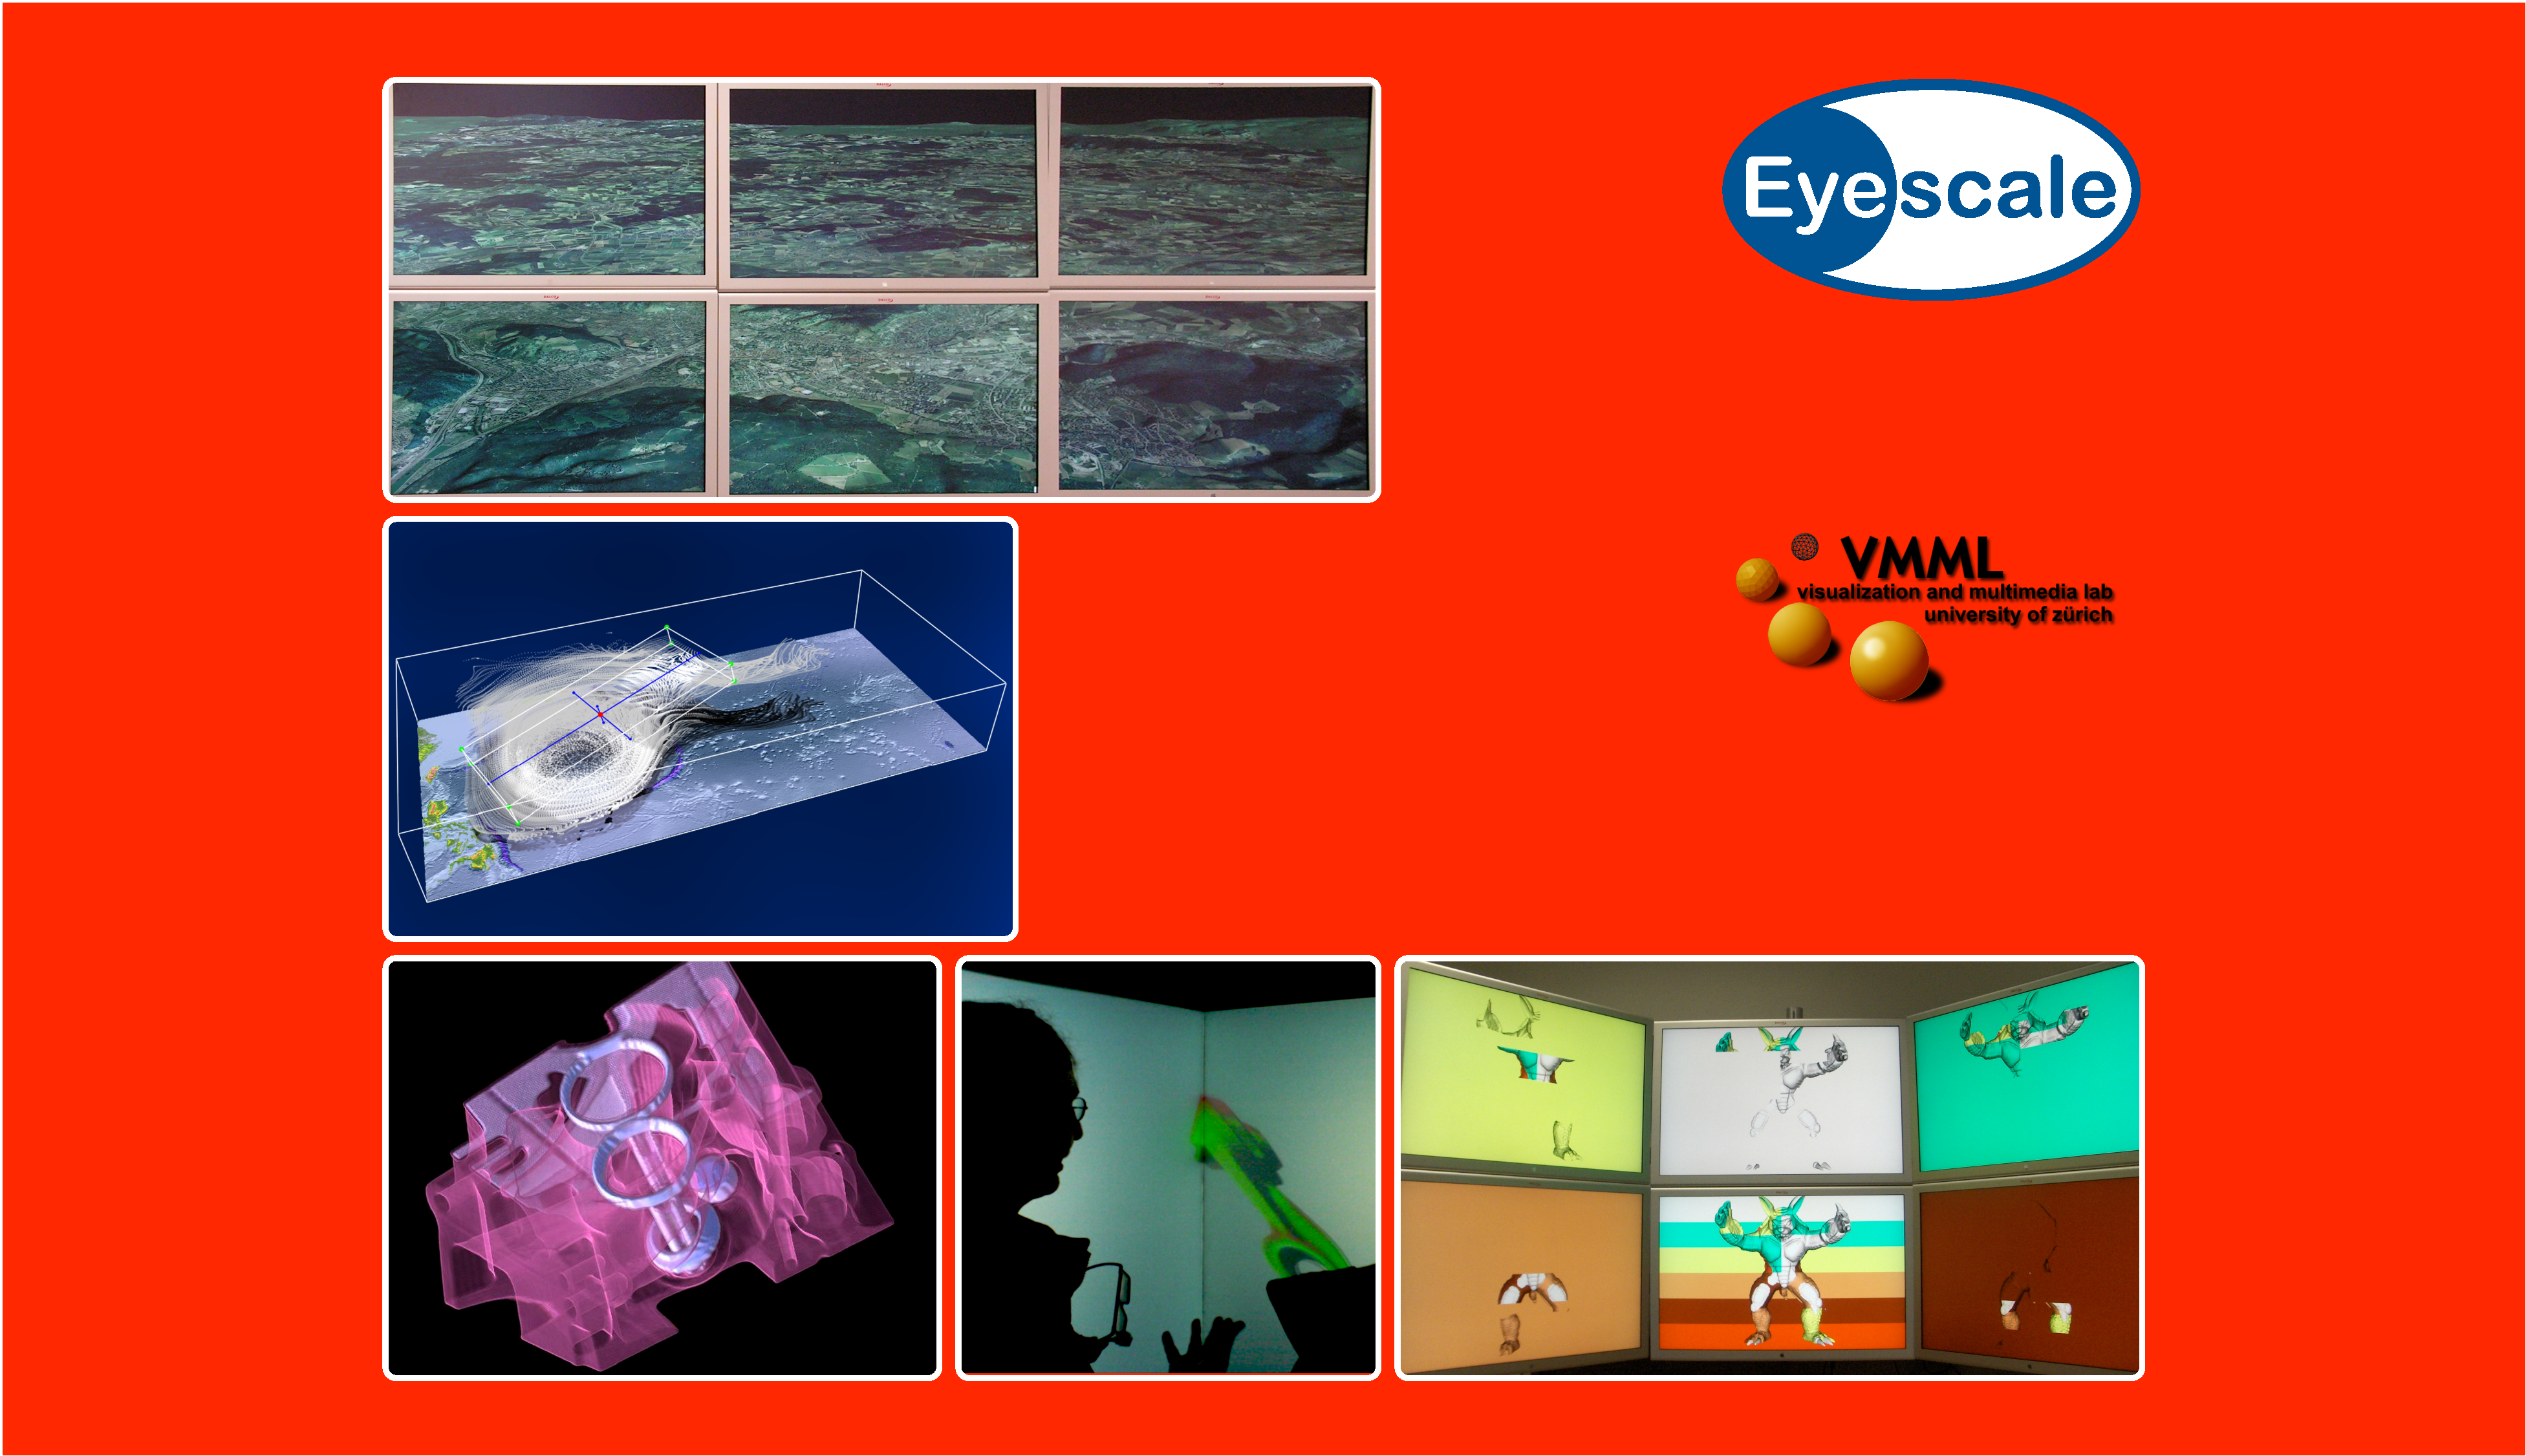
\includegraphics[width=22cm]{images/teaser.pdf}
  \end{textblock}
      {\Large The official reference for developing and
        deploying parallel, scalable OpenGL\texttrademark\ applications using
        the Equalizer parallel rendering framework}\\\vspace{1cm}
      Version 1.12 for Equalizer 1.4\\[\medskipamount]
  \today
}

\newcommand{\tm}{\texttrademark~}
\newcommand{\rc}{\raise 1ex\hbox{{\tiny\textregistered}}~}
\newcommand{\fig}[1]{Figure~\ref{#1}}
\newcommand{\sref}[1]{Section~\ref{#1}}
\newcommand{\aref}[1]{Appendix~\ref{#1}}
\newcommand{\link}[1]{\htmladdnormallink{#1}{#1}}
\indentcaption{2em}
\setcounter{tocdepth}{2}

% suppress  single floating lines on top (widow) and bottom(club)
%  10000 is infinity
%  tradeoff: maybe underfull vboxes
\clubpenalty=10000
\widowpenalty=10000

\begin{document}

\pagestyle{empty}
\maketitle
\thispagestyle{empty}

\clearpage

\lstset{language=C++}
\section*{Equalizer Programming and User Guide}
\today
\subsection*{Contributors}

Written by Stefan Eilemann.\\
Contributions by Maxim Makhinya, Jonas B\"osch, Christian Marten, Sarah
Amsellem, Patrick Bouchaud, Philippe Robert, Robert Hauck and Lucas Peetz
Dulley.

\subsection*{Copyright}

\textcopyright 2007-2012 \htmladdnormallink{Eyescale Software GmbH}
{http://www.eyescale.ch}. All rights reserved. No permission is
granted to copy, distribute, or create derivative works from the
contents of this electronic documentation in any manner, in whole or in
part, without the prior written permission of Eyescale Software GmbH.

\subsection*{Trademarks and Attributions}

OpenGL is a registered Trademark, OpenGL Multipipe is a Trademark of
Silicon Graphics, Inc. Linux is a registered Trademark of Linus
Torvalds.  Mac OS is a Trademark of Apple Inc. CAVELib is a registered
Trademark of the University of Illinois. The CAVE is a registered
Trademark of the Board of Trustees of the University of Illinois at
Chicago. Qt is a registered Trademark of Trolltech. TripleHead2Go is a
Trademark of Matrox Graphics. PowerWall is a Trademark of Mechdyne
Corporation. CUDA is a Trademark of NVIDIA Corporation. All other
trademarks and copyrights herein are the property of their respective
owners.

\subsection*{Feedback}

If you have comments about the content, accuracy or comprehensibility of
this Programming and User Guide, please contact
\htmladdnormallink{eile@eyescale.ch}
{mailto:eile@eyescale.ch?subject=Equalizer\%20Programming\%20Guide}.

\vfill

\subsection*{Front and Back Page}

The images on the front page show the following applications build using
Equalizer: RTT DeltaGen\footnote{Image copyright Realtime Technology AG, 2008}
[top right], \textsf{Bino}, a stereo-capable, multi-display video
player\footnote{\link{http://bino.nongnu.org/}} [middle center], a flow
visualization application for climate research\footnote{Image courtesy of
  Computer Graphics and Multimedia Systems, University of Siegen} [middle
  right], the \textsf{eqPly} polygonal renderer in a three-sided CAVE [bottom
  left], the \textsf{eVolve} volume renderer\footnote{Data set courtesy of
  General Electric, USA} [bottom center], and the
\textsf{RTNeuron}\footnote{Image courtesy of
  \htmladdnormallink{Cajal Blue Brain}{http://cajalbbp.cesvima.upm.es/} /
  \htmladdnormallink{Blue Brain Project}{http://bluebrain.epfl.ch}}
  application to visualize cortical circuit simulations [bottom right].

The images on the back page show the following scalable rendering modes:
Subpixel (FSAA) [top left], DPlex [middle left], Pixel [middle center],
2D [bottom left], DB [bottom center] and stereo [bottom right].

\clearpage
\pagenumbering{roman}
\pagestyle{headings}
\tableofcontents
%\clearpage
\listoffigures \vfill
\section*{Revision History}
{\center\begin{tabularx}{\textwidth}{|l|l|X|}
    \hline
    \bf Rev & \bf Date     & \bf Changes \\
    \hline
    1.0     & Oct 28, 2007 & Initial Version for Equalizer 0.4\\
    1.2     & Apr 15, 2008 & Revision for Equalizer 0.5\\
    1.4     & Nov 25, 2008 & Revision for Equalizer 0.6\\
    1.6     & Aug 07, 2009 & Revision for Equalizer 0.9\\
    1.8     & Mar 21, 2011 & Revision for Equalizer 1.0\\
    1.10    & Feb 17, 2012 & Revision for Equalizer 1.2\\
    1.12    & Jul 20, 2012 & Revision for Equalizer 1.4\\
    \hline
  \end{tabularx}}
\clearpage

\pagenumbering{arabic}

\part{User Guide}
\section{Introduction}

Equalizer is the standard middleware for the development and deployment of
parallel OpenGL applications. It enables applications to benefit from multiple
graphics cards, processors and computers to improve the rendering performance,
visual quality and display size. An Equalizer-based application runs unmodified
on any visualization system, from a simple workstation to large scale graphics
clusters, multi-GPU workstations and Virtual Reality installations.

This User and Programming Guide introduces parallel rendering concepts,
the configuration of Equalizer-based applications and programming using
the Equalizer parallel rendering framework.

Equalizer is the most advanced middleware for scalable 3D visualization,
providing the broadest set of parallel rendering features available in
an open source library to any visualization application. Many commercial and
open source applications in a variety of different markets rely on
Equalizer for flexibility and scalability.

Equalizer provides the domain-specific parallel rendering expertise and
abstracts configuration, threading, synchronization, windowing and event
handling. It is a `GLUT on steroids', providing parallel and distributed
execution, scalable rendering features, an advanced network library and fully
customizable event handling.

If you have any question regarding Equalizer programming, this guide, or
other specific problems you encountered, please direct them to the
\textsf{eq-dev} mailing
list\footnote{\link{http://www.equalizergraphics.com/lists.html}}.


\subsection{Parallel Rendering}

\begin{wrapfigure}{r}{.618\textwidth}
  \vspace{-1ex}\includegraphics[width=.618\textwidth]{images/executionFlow.pdf}
  {\caption{\label{fExecutionFlow}Parallel Rendering}}
  \vspace{-4ex}
\end{wrapfigure}

\fig{fExecutionFlow} illustrates the basic principle of any parallel rendering
application. The typical OpenGL application, for example using GLUT, has an
event loop which redraws the scene, updates application data based on received
events, and eventually renders a new frame.

A parallel rendering application uses the same basic execution model, extending
it by separating the rendering code from the main event loop. The rendering code
is then executed in parallel on different resources, depending on the
configuration chosen at runtime.

This model is naturally followed by Equalizer, thus making application
development as easy as possible.


\subsection{Installing Equalizer and Running \textsf{eqPly}}

Equalizer can be installed by downloading a binary installer or source
code\footnote{\link{http://www.equalizergraphics.com/downloads.html}}. After
installing Equalizer, please take a look at the Quickstart
Guide\footnote{\link{http://www.equalizergraphics.com/documents/EqualizerGuide.html}}
to get familiar with the capabilities of Equalizer and the \textsf{eqPly}
example.

Equalizer uses CMake to generate platform-specific build files. Compiling
Equalizer from source is as simple as running \textsf{make} on Linux or Mac OS
X, running \textsf{make xcode} and building the generated XCode project on Mac
OS X, or creating a Equalizer Visual Studio solution using \textsf{CMake} on
Windows.

\subsection{Equalizer Processes}

The Equalizer architecture is based on a client-server model. The client
library exposes all functionality discussed in this document to the
programmer, and provides communication between the different Equalizer
processes.

\begin{wrapfigure}{r}{.382\textwidth}
  \includegraphics[width=.382\textwidth]{images/processes.pdf}
  {\caption{\label{fProcesses}Equalizer Processes}}
\end{wrapfigure}
Collage is a cross-platform C++ library for building heterogeneous, distributed
applications. Collage provides an abstraction of different network connections,
peer-to-peer messaging, discovery and synchronization as well as
high-performance, object-oriented, versioned data distribution. Collage is
designed for low-overhead multi-threaded execution which allows applications to
easily exploit multi-core architectures. Equalizer uses Collage as the cluster
backend, e.g., by setting up direct communication between two nodes when needed
for image compositing or software swap barriers.

\fig{fProcesses} depicts the relationship between the server, application,
render client and administrative processes, which are explained below.

\subsubsection{Server}
The Equalizer server is responsible for managing one visualization session on a
shared memory system or graphics cluster. Based on its configuration and
controlling input from the application, it computes the active resources,
updates the configuration and generates tasks for all processes. Furthermore it
controls and launches the application's rendering client processes. The
Equalizer server is the entity in charge of the configuration, and all other
processes receive their configuration from the server.

\subsubsection{Application}

The application connects to an Equalizer server and receives a configuration.
Furthermore, the application also provides its render client, which will be
controlled by the server. The application and render client may use the same
executable. The application has a main loop, which reacts on events, updates its
data and controls the rendering.

\subsubsection{Render Clients}

The render client implements the rendering part of an application. Its execution
is passive, it has no main loop and is completely driven by Equalizer server. It
executes the rendering tasks received from the server by the calling the
appropriate task methods (see \sref{sTaskMethods}) in the correct thread and
context. The application either implements the task methods with
application-specific code or uses the default methods provided by Equalizer.

The application can also be a rendering client, in which case it can
also contribute to the rendering. If it does not implement any render
client code, it is reduced to be the application's `master' process
without any OpenGL windows and 3D rendering.

The rendering client can be the same executable as the application, as
it is the case with all provided examples. When it is started as a
render client, the Equalizer initialization routine does not return and
takes over the control by calling the render client task
methods. Complex applications usually implement a separate, lightweight
rendering client.

\subsubsection{Administration Programs}

Equalizer 1.0 introduced the admin library, which can be used to modify a
running Equalizer server. The admin library is still in development, but already
allows limited modifications such as adding new windows and changing
layouts. The admin library may be used to create standalone administration tools
or from within the application code. In any case, it has an independent view of
the server's configuration. Documentation for admin library is not yet part of
this Programming and User Guide.


\section{Scalable Rendering}

Scalable rendering is a subset of parallel rendering, where more multiple
resources are used to update a view.

Real-time visualization is an inherently parallel problem. Different
applications have different rendering algorithms, which require different
scalable rendering modes to address the bottlenecks correctly. Equalizer
supports all important algorithms as listed below, and will continue to add new
ones over time to meet application requirements.

This section gives an introduction to scalable rendering, providing some
background for end users and application developers. The scalability
modes offered by Equalizer are discussed, along with their advantages
and disadvantages.

Choosing the right mode for the application profile is critical for
performance. Equalizer uses the concept of compounds to describe the
task decomposition and result recomposition. It allows the combination
of the different compound modes in any possible way, which allows to
address different bottlenecks in a flexible way.


\subsection{2D or Sort-First Compounds}

\begin{wrapfigure}{r}{.618\textwidth}
  \includegraphics[width=.618\textwidth]{images/2D.pdf}
  {\caption{2D Compound}}
\end{wrapfigure}
2D decomposes the rendering in screen-space, that is, each contributing
rendering unit processes a tile of the final view. The recomposition
simply assembles the tiles side-by-side on the destination view. This
mode is also known as sort-first or SFR.

The advantage of this mode is a low, constant IO overhead for the pixel
transfers, since only color information has to be transmitted. The upper
limit is the amount of pixel data for the destination view.

Its disadvantage is that it relies on view frustum culling to reduce the
amount of data submitted for rendering. Depending on the application
data structure, the overlap of some primitives between individual tiles
limits the scalability of this mode, typically to around eight graphics
cards. Each node has to potentially hold the full database for
rendering.

2D decompositions can be used by all types of applications, but should
be combined with DB compounds to reduce the data per node, if
possible. In most cases, a \textsf{load\_equalizer} should be used to
automatically adjust the tiling each frame, based on the current
rendering load.

2D compounds in Equalizer are configured using the \textsf{viewport}
parameter, using the values \textsf{[ x y width height]} in normalized
coordinates. The viewport defines the area of the parent (destination)
channel to be rendered for each child. Each child compound uses an
output frame, which is connected to an input frame on the destination
channel. The destination channel can also be used as a source channel,
in which case it renders in place and no output frame is needed.

\subsection{DB or Sort-Last Compounds}

DB, as shown in \fig{fDB}\footnote{3D model courtesy of AVS, USA.}, decomposes
the rendered database so that all rendering units process a part of the scene in
parallel. This mode is also known as sort-last, and is very similar to the data
decomposition approach used by HPC applications.

\begin{wrapfigure}{r}{.618\textwidth}
  \includegraphics[width=.618\textwidth]{images/DB.pdf}
  {\caption{\label{fDB}Database Compound}}
\end{wrapfigure}
Volume rendering applications use an ordered alpha-based blending to
composite the result image. The depth buffer information is used to
composite the individual images correctly for polygonal data.

This mode provides very good scalability, since each rendering unit
processes only a part of the database. This allows to lower the
requirements on all parts of the rendering pipeline: main memory usage,
IO bandwidth, GPU memory usage, vertex processing and fill rate.

Unfortunately, the database recomposition has linear increasing IO
requirements for the pixel transfer. Parallel compositing algorithms,
such as direct-send, address this problem by keeping the per-node IO
constant (see \fig{fDirectSend}).

The application has to partition the database so that the rendering units render
only part of the database. Some OpenGL features do not work correctly
(anti-aliasing) or need special attention (transparency, shadows).

The best use of database compounds is to divide the data to a manageable
size, and then to use other decomposition modes to achieve further
scalability. Volume rendering is one of the applications which can
profit from database compounds.

DB compounds in Equalizer are configured using the \textsf{range}
parameter, using the values \textsf{[ begin end ]} in normalized
coordinates. The range defines the start and end point of the
application's database to be rendered. The value has to be interpreted
by the application's rendering code accordingly.  Each child compound
uses an output frame, which is connected to an input frame on the
destination channel. For more than two contributing channels, it is
recommended to configure streaming or parallel direct send compositing,
as described in \sref{sDirectSend}.


\subsection{Stereo Compounds}

Stereo compounds, as shown in \fig{fStereoCmp}\footnote{3D model
  courtesy of Stereolithography Archive at Clemson University.}, assign
each eye pass to individual rendering units. The resulting images are
copied to the appropriate stereo buffer. This mode supports a variety of
stereo modes, including active (quad-buffered) stereo, anaglyphic stereo
and auto-stereo displays with multiple eye passes.

\begin{wrapfigure}{r}{.618\textwidth}
  \includegraphics[width=.618\textwidth]{images/EYE.pdf}
  {\caption{\label{fStereoCmp}Stereo Compound}}
\end{wrapfigure}
Due to the frame consistency between the eye views, this modes scales very
well. The IO requirements for pixel transfer are small and constant. The number
of rendering resources used by stereo compounds is limited by the number of eye
passes, typically two.

Stereo compounds are used by all applications when rendering in stereo,
and is often combined with other modes.

Eye compounds in Equalizer are configured using the \textsf{eye}
parameter, limiting the child to render the \textsf{[ LEFT ]} or
\textsf{[ RIGHT ]} eye. Each child compound uses an output frame, which
is connected to an input frame on the destination channel. The
destination channel can also be used to render an eye pass, in which case
it renders in the correct stereo buffer and no output frame is needed.


\subsection{\label{sDPlex}DPlex Compounds}

\begin{wrapfigure}{r}{.618\textwidth}
  \vspace{-2ex}
  \includegraphics[width=.618\textwidth]{images/DPlex.pdf}
  {\caption{A DPlex Compound}}
\end{wrapfigure}
DPlex compounds assign full, alternating frames to individual rendering
units. The resulting images are copied to the destination channel, and
Equalizer load-balancing is used to ensure a steady framerate on the
destination window. This mode is also known as time-multiplex or AFR.

Due to the frame consistency between consecutive frames, this mode scales
very well. The IO requirements for pixel transfer are small and
constant.

DPlex requires a latency of at least n frames. This increased latency
might be disturbing to the user, but it is often compensated by the
higher frame rate. The frame rate typically increases linearly with the
number of source channels, and therefore linearly with the latency.

DPlex compounds in Equalizer are configured using the \textsf{period}
and \textsf{phase} parameter, limiting each child to render a subset of
the frames. Each child compound uses an output frame, which is connected
to an input frame on the destination channel. The destination channel
uses a \textsf{framerate\_equalizer} to smoothen the framerate.


\subsection{\label{sTileCompunds}Tile Compounds}

Tile compounds are similar to 2D compounds. They decompose the rendering in
screen-space, where each rendering unit pulls and processes regular tiles of the
final view. Tile compounds are ideal for purely fill-limited applications such
as volume rendering and raytracing.

\begin{wrapfigure}{r}{.618\textwidth}
  \includegraphics[width=.618\textwidth]{images/tile.pdf}
  {\caption{\label{fTile}Tile Compound}}
\end{wrapfigure}
Tile compounds have a low, constant IO overhead for the image transfers and can
provide good scalability when used with fill-limited applications. Tile
decomposition works transparently for all Equalizer-based applications.

Contrary to all other compounds, the work distribution is not decided
before-hand using a push model, but each resource pulls work from a central work
queue, until all tiles have been processed. Therefore the rendering is naturally
load-balanced since all sources pull data on an as-needed basis. The queue
implementation uses prefetching to hide the communication overhead of the
central, distributed tile queue.

\subsection{Pixel Compounds}

\begin{wrapfigure}{r}{.618\textwidth}
  \vspace{-2ex}\includegraphics[width=.618\textwidth]{images/Pixel.pdf}
  {\caption{\label{fPixel}Pixel Compound}}\vspace{-8ex}
\end{wrapfigure}
Pixel compounds are similar to 2D compounds. While 2D compounds decompose the
screen space into contiguous regions, pixel compounds assign one pixel of a
regular kernel to each resource. The frusta of the source rendering units are
modified so that each unit renders an evenly distributed subset of pixels, as
shown in \fig{fPixel}\footnote{3D model courtesy of AVS, USA.}

As 2D compounds, pixel compounds have low, constant IO requirements for the
pixel transfers during recomposition. They are naturally load-balanced for
fill-limited operations, but do not scale geometry processing at all.

OpenGL functionality influenced by the raster position will not work
correctly with pixel compounds, or needs at least special
attention. Among them are: lines, points, sprites, glDrawPixels,
glBitmap, glPolygonStipple. The application can query the current pixel
parameters at runtime to adjust the rendering accordingly.

\begin{wrapfigure}{l}{.382\textwidth}
  \includegraphics[width=.382\textwidth]{images/pixelKernel.pdf}
  {\caption{\label{fPixelKernel}\small Pixel Compound Kernel}}
\end{wrapfigure}
Pixel compounds work well for purely fill-limited applications. Techniques like
view frustum culling do not reduce the rendered data, since each resource has
approximately the same frustum. Pixel compounds are ideal for ray-tracing, which
is highly fill-limited and needs the full database for rendering anyway. Volume
rendering applications are also well suited for this mode, and should choose it
over 2D compounds.

Pixel compounds in Equalizer are configured using the \textsf{pixel}
parameter, using the values \textsf{[ x y width height]}  to configure
the size and offset of the sampling kernel. The width and height of the
sampling kernel define how many pixels are skipped in the x and y
direction, respectively. The x and y offset define the index of the
source channel within the kernel. They have to be smaller than the size
of the kernel. \fig{fPixelKernel} illustrates these parameters, and
\fig{fPixelKernels} shows some example kernels for a four-to-one pixel decomposition.

The destination channel can also be used as a source channel. Contrary
to the other compound modes, it also has to use an output and
corresponding input frame. During rendering, the frustum is 'squeezed'
to configure the pixel decomposition. The destination channel can
therefore not be rendered in place, like with the other compound modes.
\begin{figure}[ht!]\center
  \includegraphics[width=.9\textwidth]{images/pixelKernels.pdf}
  {\caption{\label{fPixelKernels}Example Pixel Kernels for a
      four-to-one Pixel Compound}}
\end{figure}


\subsection{\label{sSubpixel}Subpixel Compounds}

Subpixel decomposes the rendering of multiple samples for one pixel, e.g., for
anti-aliasing or depth-of-field rendering. The default implementation provides
transparent, scalable software idle-antialiasing when configuring a subpixel
compound.

Applications can use subpixel compounds to accelerate depth-of-field effects and
software anti-aliasing, with potentially a different number of idle or non-idle
samples per pixel.

As for the DB compound, the subpixel recomposition has linear increasing
IO requirements for the pixel transfer, with the difference that only
color information has to be transmitted.

\begin{wrapfigure}{r}{.618\textwidth}
  \includegraphics[width=.618\textwidth]{images/Subpixel.pdf}
  {\caption{\label{fSubpixel}Subpixel Compound}}
\end{wrapfigure}
Subpixel compounds are configured using the \textsf{subpixel} parameter, using
the values \textsf{[~index size ]}. The \textsf{index} parameter corresponds to
the current resource index and the \textsf{size} is the total number of
resources used.

The \textsf{index} has to be smaller than the \textsf{size}.
\fig{fSubpixel} illustrates a three-way subpixel decomposition.

The destination channel can also be used as a source channel.
As for the pixel compound, it has to use an output and corresponding
input frame.


\subsection{\label{sLoadBalancing}Automatic Runtime Adjustments}

Some scalable rendering parameters are updated at runtime to provide
optimal performance or influence other scalable rendering
features. These adjustments are often referred to as load-balancing, but
are called \textsf{equalizers}, since their functionality is not limited
to load-balancing in Equalizer.

The server provides a number of equalizers, which automatically update
certain parameters of compounds based on runtime information. They
balance the load of 2D and DB compounds, optimally distribute render
resources for multi-display projection systems, adjust the resolution
to provide a constant framerate or zoom images to allow monitoring of
another view.

Equalizers are described in more detail in \sref{sEqualizers}.


\section{\label{sConfig}Configuring Equalizer Clusters}

\subsection{\label{sAutoConfig}Auto-Configuration}

\subsubsection{Hardware Service Discovery}

Equalizer uses the hwsd library for discovering local and remote GPUs and
network interfaces. Based on this information, a typical configuration is
dynamically compiled during the initialization of the application. The
auto-configuration uses the same format as the static configuration files. It
can be used to create template configurations by running a test application or
the eqServer binary and using the generated configuration, saved as
\textless session\textgreater.auto.eqc.

Please note that both hwsd and the hwsd ZeroConf module are optional and
requires hwsd and a ZeroConf implementation when Equalizer is compiled.

hwsd contains three components: a core library, local and remote discovery
modules as well as a ZeroConf daemon. The daemon uses the appropriate module to
query local GPUs and network interfaces and announces them using ZeroConf on the
local network.

\begin{wrapfigure}{r}{.618\textwidth}
  \includegraphics[width=.618\textwidth]{images/gpu-sd.pdf} % TODO: update image (hwsd)
  {\caption{\label{fHWSD}GPU discovery for auto-configuration}}
\end{wrapfigure}
Equalizer uses the library with the dns\_sd discovery module to gather the
information announced by all daemons on the local network, as well as the local
discovery modules for standalone auto-configuration. The default configuration
is using all locally discovered GPUs and network interfaces.

\fig{fHWSD} shows how hwsd is used to discover four remote GPUs on two
different machines to use them to render a single view on a laptop.

\subsubsection{\label{sHWSDUsage}Usage}

On each node contributing to the configuration, install and start the hwsd
daemon. If multiple, disjoint configurations are used on the same network,
provide the session name as a parameter when starting the daemon. Verify that
all GPUs and network interfaces are visible on the application host using
the \textsf{hw\_sd\_list} tool. When starting the application, use the
command-line parameter \textsf{--eq-config}:

\begin{itemize}
\item The default value is \textsf{local} which uses all local GPUs and network
  interfaces queried using the cgl, glx, or wgl GPU module and the sys network
  module.
\item \textsf{--eq-config sessionname} uses the dns\_sd ZeroConf module of
  hwsd to query all GPUs and network interfaces in the subnet for the given
  session. The default session of the hwsd daemon is \textsf{default}. The
  found network interfaces are used to connect the nodes.
\item \textsf{--eq-config filename.eqc} loads a static configuration from the
  given ASCII file. The following sections describe how to write configuration
  files.
\end{itemize}

The auto-configuration creates one display window on the local machine, and one
off-screen channel for each GPU. The display window has one full-window channel
used as an output channel for a single segment. It combines all GPUs into a
scalability config with different layouts for each of the following scalability
modes:

\begin{description}
\item [2D] A dynamically load-balanced sort-first configuration using all GPUs
  as sources.
\item [Simple] A no-scalability configuration using only the display GPU for
  rendering.
\item [Static DB] A static sort-last configuration distributing the range evenly
  across all GPUs.
\item [Dynamic DB] A dynamically load-balanced sort-last configuration using all
  GPUs as sources.
\item [DB Direct Send] A direct send sort-last configuration using all GPUs as
  sources.
\item [DB 2D] A direct send sort-last configuration using all nodes together
  with a dynamically load-balanced sort-first configuration using local GPUs.
\end{description}

All suitable network interfaces are used to configure the node, that is, the
launch command has to be able to resolve one hostname for starting the render
client processes. Suitable interfaces have to be up and match optional given
values which can be specified by the following command-line parameters:

\begin{description}
\item[--eq-config-flags \textless ethernet\textbar infiniband\textgreater]
  Limit the selection of network interfaces to one of the those types.
\item[--eq-config-prefixes \textless CIDR-prefixes\textgreater] Limit the
  selection of network interfaces that match the given prefix.
\end{description}

\subsection{Preparation}

Before writing a configuration, it is useful to assemble the following
information:

\begin{itemize}
\item A list of all \textbf{computers} in your rendering cluster,
  including the \textbf{IP addresses} of all network interfaces to be
  used.
\item The number of \textbf{graphics cards} in each computer.
\item The \textbf{physical dimensions} of the display system, if
  applicable. These are typically the bottom-left, bottom-right and
  top-left corner points of each display surface in meters.
\item The relative coordinates of all the \textbf{segments} belonging to
  each display surface, and the graphics card \textbf{output} used for
  each segment. For homogeneous setups, it is often enough to know the
  number of rows and columns on each surface, as well as the overlap or
  underlap percentage, if applicable.
\item The number of desired \textbf{application windows}. Application
  windows are typically destination windows for scalable rendering or
  'control' windows paired with a view on a display system.
\item \textbf{Characteristics} of the application, e.g., supported
  scalability modes and features.
\end{itemize}

\subsection{Summary}

Equalizer applications are configured at runtime by the Equalizer
server. The server loads its configuration from a text file, which is a
one-to-one representation of the configuration data structures at
runtime.

For an extensive documentation of the file format please refer to
\aref{aFileFormat}. This section gives an introduction on how to write
configuration files.

A configuration consists of the declaration of the rendering resources, the
description of the physical layout of the projection system, logical layouts on
the projection canvases and an optional decomposition description using the
aforementioned resources.

The rendering resources are represented in a hierarchical tree structure
which corresponds to the physical and logical resources found in a 3D
rendering environment: nodes (computers), pipes (graphics cards),
windows, channels.

Physical layouts of display systems are configured using canvases with
segments, which represent 2D rendering areas composed of multiple
displays or projectors. Logical layouts are applied to canvases and
define views on a canvas.

Scalable resource usage is configured using a compound tree, which is a
hierarchical representation of the rendering decomposition and
recomposition across the resources.

\begin{figure}[ht!]\center
  \includegraphics[width=\textwidth]{images/cave.pdf}
  {\caption{\label{fConfig}An Example Configuration}}
\end{figure}

\fig{fConfig} shows an example configuration for a four-side
CAVE, running on two machines (nodes) using three graphics
cards (pipes) with one window each to render to the four output channels
connected to the projectors for each of the walls.

For testing and development purposes it is possible to use multiple
instances for one resource, e.g. to run multiple render client nodes on
one computer. For optimal performance during deployment, one node and
pipe should be used for each computer and graphics card, respectively.

\subsection{Node}

For each machine in your cluster, create one \textsf{node}. Create one
\textsf{appNode} for your application process. List all nodes, even if you are
not planning to use them at first. Equalizer will only instantiate and access
used nodes, that is, nodes which are referenced by an active compound.

In each node, list all \textsf{connection}s through which this node is
reachable. Typically a node uses only one connection, but it is possible
to configure multiple connections if the machine and cluster is set up
to use multiple, independent network interfaces. Make sure the
configured \textsf{hostname} is reachable from all nodes. An IP address
may be used as the hostname.

For cluster configurations with multiple nodes, configure at least one
connection for the server. All render clients connect back to the server, for
which this connection is needed.

The \textsf{eq::Node} class is the representation of a single computer
in a cluster. One operating system process of the render client will be
used for each node. Each configuration might also use an application
node, in which case the application process is also used for
rendering. All node-specific task methods are executed from the main
application thread.

\subsection{Pipe}

For each node, create one \textsf{pipe} for each graphics card in the
machine. Set the \textsf{device} number to the correct index. On
operating systems using X11, e.g., Linux, also set the port number if
your X-Server is running on a nonstandard port.

The \textsf{eq::Pipe} class is the abstraction of a graphics card (GPU), and
uses one independent operating system thread for rendering. Non-threaded pipes
are supported for integrating with thread-unsafe libraries, but have various
performance caveats. They should only be used if using a different, synchronized
rendering thread is not an option.

All pipe, window and channel task methods are executed from the pipe
thread, or in the case of non-threaded pipes from the main application
thread\footnote{see
  \link{http://www.equalizergraphics.com/documents/design/nonthreaded.html}}.

\subsection{Window}

Configure one \textsf{window} for each desired application window on the
appNode. Configure one full-screen window for each display
segment. Configure one off-screen window, typically a pbuffer, for each
graphics card used as a source for scalable rendering. Provide a useful
name to each on-screen window if you want to easily identify it at runtime.

Sometimes display segments cover only a part of the graphics card
output. In this case it is advised to configure a non-fullscreen window
without window decorations, using the correct window viewport.

The \textsf{eq::Window} class encapsulates a drawable and an OpenGL
context. The drawable can be an on-screen window or an off-screen
pbuffer or framebuffer Object (FBO).

\subsection{Channel}

Configure one \textsf{channel} for each desired rendering area in each
window. Typically one full-screen channel per window is used. Name the
channel using a unique, easily identifiable name, e.g., 'source-1',
'control-2' or 'segment-2\_3'.

Multiple channels in application windows may be used to view the model
from different viewports.

Sometimes, a single window is split across multiple projectors, e.g., by
using an external splitter such as the Matrox TripleHead2Go. In this
case configure one channel for each segment, using the channel's
\textsf{viewport} to configure its position relative to the window.

The \textsf{eq::Channel} class is the abstraction of an OpenGL viewport
within its parent window. It is the entity executing the actual
rendering. The channel's viewport is overwritten when it is rendering
for another channel during scalable rendering.


\subsection{\label{sCanvas}Canvases}

\begin{wrapfigure}{r}{.618\textwidth}
  \includegraphics[width=.618\textwidth]{images/frusta.pdf}
  {\caption{\label{fFrusta}Wall and Projection Parameters}}
\end{wrapfigure}
If you are writing a configuration for workstation usage you can skip
the following sections and restart with \sref{sCompounds}.

Configure one \textsf{canvas} for each display surface. For planar
surfaces, e.g., a display wall, configure a frustum. For non-planar
surfaces, the frustum will be configured on each display segment.

The frustum can be specified as a wall or projection description. Take
care to choose your reference system for describing the frustum to be
the same system as used by the head-tracking matrix calculated by the
application.

A wall is completely defined by the bottom-left, bottom-right and
top-left coordinates relative to the origin.

A projection is defined by the position and head-pitch-roll orientation
of the projector, as well as the horizontal and vertical field-of-view
and distance of the projection wall.

\fig{fFrusta} illustrates the wall and projection frustum parameters.

A canvas represents one physical projection surface, e.g., a PowerWall, a
curved screen or an immersive installation. One configuration might
drive multiple canvases, for example an immersive installation and an
operator station.

A canvas consists of one or more segments. A planar canvas typically has
a frustum description (see \sref{sFrustum}), which is inherited by the
segments. Non-planar frusta are configured using the segment
frusta. These frusta typically describe a physically correct display
setup for Virtual Reality installations.

A canvas has one or more layouts. One of the layouts is the active
layout, that is, this set of views is currently used for rendering. It
is possible to specify \textsf{OFF} as a layout, which deactivates the
canvas. It is possible to use the same layout on different canvases.

A canvas may have a swap barrier, which is used as the default swap barrier by
all its segments to synchronize the video output.

Canvases provide a convenient way to configure projection surfaces. A canvas
uses layouts, which describe logical views. Typically, each desktop window uses
one canvas, one segment, one layout and one view.

\subsubsection{Segments}

Configure one \textsf{segment} for each display or projector of each
canvas. Configure the \textsf{viewport} of the segment to match the area
covered by the segment on the physical canvas. Set the output
\textsf{channel} to the resource driving the described projector.

For non-planar displays, configure the frustum as described in
\sref{sCanvas}. For passive stereo installations, configure one segment per eye
pass, where the segment for the left and right eye have the same viewport. Set
the eyes displayed by the segment, i.e., left or right and potentially cyclop.

\begin{wrapfigure}{r}{.382\textwidth}
  \includegraphics[width=.382\textwidth]{images/canvas.pdf}
  {\caption{\label{fCanvas}A Canvas using four Segments}}
\end{wrapfigure}
To synchronize the video output, configure either a canvas swap barrier or a
swap barrier on each segment to be synchronized.

When using software swap synchronization, swap-lock all segments using a swap
barrier. All windows with a swap barrier of the same name synchronize their
swapbuffers. Software swap synchronization uses a distributed barrier, and works
on all hardware.

When using hardware swap synchronization, use swap barriers for all segment to
be synchronized, setting \textsf{NV\_group} and \textsf{NV\_barrier}
appropriately. The swap barrier name is ignored in this case. All windows of the
same group on a single node synchronize their swap buffer. All groups of the
same barrier synchronize their swap buffer across nodes. Please note that the
driver typically limits the number of groups and barriers to one, and that
multiple windows per swap group are not supported by all drivers. Hardware swap
barriers require support from the OpenGL driver, and has been tested on NVIDIA
Quadro GPUs with the G-Sync option. Please refer to your OpenGL driver
documentation for details.

A segment represents one output channel of the canvas, e.g., a projector
or an LCD. A segment has an output channel, which references the channel to
which the display device is connected.

A segment covers a part of its parent canvas, which is configured using the
segment viewport. The viewport is in normalized coordinates relative to the
canvas. Segments might overlap (edge-blended projectors) or have gaps between
each other (display walls, \fig{fCanvas}\footnote{Dataset courtesy of VolVis
  distribution of SUNY Stony Brook, NY, USA.}). The viewport is used to
configure the segment's default frustum from the canvas frustum description, and
to place layout views correctly.

\subsubsection{\label{sSwapBarrier}Swap and Frame Synchronization}
Canvases and segments may have a software or hardware swap barrier to
synchronize the buffer swap of multiple channels. The swap barriers are
inherited from the canvas to the segment ultimately to all compounds using a
destination channel of the segment.

A software swap barrier is configured by giving it a name. Windows with a swap
barrier of the same name synchronize with each other before executing the swap
buffer task. Before entering the barrier, \textsf{Window::finish} is called to
ensure that all OpenGL commands have been executed.  Swap barrier names are only
valid within the compound tree, that is, a compound from one compound tree
cannot be synchronized with a compound from another compound tree.

A hardware swap barrier uses a hardware component to synchronize the buffer swap
of multiple windows. It guarantees that the swap happens at the same vertical
retrace of all corresponding video outputs.  It is configured by setting the
\textsf{NV\_group} and \textsf{NV\_barrier} parameters. These parameters follow
the \textsf{NV\_swap\_group} extension, which synchronizes all windows bound to
the same group on a single machine, and all groups bound to the same barrier
across systems.

Display synchronization uses different algorithms. Framelock synchronizes each
vertical retrace of multiple graphic outputs using a hardware component. This is
configured in the driver, independently of the application. Genlock synchronizes
each horizontal and vertical retrace of multiple graphic outputs, but is not
commonly used anymore for 3D graphics. Swap lock synchronizes the front and back
buffer swap of multiple windows, either using a software solution based on
network communication or a hardware solution based on a physical cable. It is
independent of, but often used in conjunction with framelock.

Framelock is used to synchronize the vertical retrace in multi-display active
stereo installations, e.g., for edge-blended projection systems or immersive
installations. It is combined with a software or hardware swap barrier. Software
barriers in this case cannot guarantee that the buffer swap of all outputs
always happens with the same retrace. The time window for an output to miss the
retrace for the buffer swap is however very small, and the output will simply
swap on the next retrace, typically in 16 milliseconds.

Display walls made out of LCDs, monoscopic or passive stereo projection systems
often only use a software swap barrier and no framelock. The display bezels make
it very hard to notice the missing synchronization.

\subsection{\label{sLayout}Layouts}

Configure one \textsf{layout} for each configuration of logical
views. Name the layout using a unique name. Often only one layout with a
one view is used for all canvases.

Enable the layout on each desired canvas by adding it to the
canvas. Since canvases reference layouts by name or index, layouts have
to be configured before their respective canvases in the configuration
file.

A layout is the grouping of logical views. It is used by one or more
canvases. For all given layout/canvas combinations, Equalizer creates
destination channels when the configuration file is loaded. These
destination channels can be referenced by compounds to configure
scalable rendering.

Layouts can be switched at runtime by the application. Switching a
layout will activate different destination channels for rendering.

\subsubsection{Views}

Configure one \textsf{view} for each logical view in each layout. Set the
\textsf{viewport} to position the view. Set the mode to stereo if appropriate.

A view is a logical view of the application data, in the sense used by
the Model-View-Controller pattern. It can be a scene, viewing mode,
viewing position, or any other representation of the application's data.

\begin{wrapfigure}{r}{.382\textwidth}
  \includegraphics[width=.382\textwidth]{images/layout.png}
  {\caption{\label{fLayout}Layout with four Views}}
\end{wrapfigure}
A view has a fractional viewport relative to its layout.  A layout
is often fully covered by its views, but this is not a requirement.

Each view can have a frustum description. The view's frustum overrides
frusta specified at the canvas or segment level. This is typically used
for non-physically correct rendering, e.g., to compare two models
side-by-side on a canvas. If the view does not specify a frustum, it
will use the sub-frustum resulting from the covered area on the canvas.

A view might have an observer, in which case its frustum is tracked by
this observer.

\fig{fLayout} shows an example layout using four views on a single
segment. \fig{fDisplay} shows a real-world setup of a single canvas with six
segments using underlap, with a two-view layout activated. This configuration
generates eight destination channels.

\begin{figure}[ht!]\center
  \includegraphics[width=.9\textwidth]{images/wallLayout.jpg}
  {\label{fDisplay}\caption{Display Wall using a six-Segment Canvas with a two-View Layout}}
\end{figure}

\subsection{Observers}

Unless you have multiple tracked persons, or want to disable tracking on
certain views, you can skip this section.

Configure one \textsf{observer} for each tracked person in the
configuration. Most configurations have at most one observer. Assign the
observer to all views which belong to this observer. Since the observer
is referenced by its name or index, it has to be specified before the
layout in the configuration file.

Views with no observer are not tracked. The config file loader will
create one default observer and assign it to all views if the
configuration has no observer.

An observer represents an actor looking at multiple views. It has a head matrix,
defining its position and orientation within the world, an eye separation and
focus distance parameters. Typically, a configuration has one
observer. Configurations with multiple observers are used if multiple,
head-tracked users are in the same configuration session, e.g., a non-tracked
control host with two tracked head-mounted displays.

\subsection{\label{sCompounds}Compounds}

Compound trees are used to describe how multiple rendering resources are
combined to produce the desired output, especially how multiple GPUs are
aggregated to increase the performance.

It is advised to study and understand the basic configuration files shipped with
the Equalizer configuration, before attempting to write compound
configurations. The auto-configuration code and command line program
\textsf{configTool}, shipped with the Equalizer distribution, creates some
standard configurations automatically. These are typically used as templates for
custom configuration files.

For configurations using canvases and layouts without scalability, the
configuration file loader will create the appropriate compounds. It is
typically not necessary to write compounds for this use case.

The following subsection outlines the basic approach to writing
compounds. The remaining subsections provide an in-depth explanation of
the compound structure to give the necessary background for compound
configuration.

\subsubsection{Writing Compounds}
The following steps are typically taken when writing compound
configurations:
\begin{description}
\item [Root compound] Define an empty top-level compound when
  synchronizing multiple destination views. Multiple destination views
  are used for multi-display systems, e.g., a PowerWall or CAVE. All
  windows used for one display surface should be swap-locked (see below)
  to provide a seamless image. A single destination view is typically
  used for providing scalability to a single workstation window.
\item [Destination compound(s)] Define one compound for each destination
  channel, either as a child of the empty group, or as a top-level compound. Set
  the destination channel by using the canvas, segment, layout and view name or
  index. The compound frustum will be calculated automatically based on the
  segment or view frustum. Note that one segment may created multiple
  view/segment channels, one for each view intersection of each layout used on
  the canvas. Only the compounds belonging to the active layout of a canvas are
  active at runtime.
\item[Scalability] If desired, define scalability for each of your
  destination compounds. Add one compound using a source channel for
  each contributor to the rendering. The destination channel may also be
  used as a source.
  \begin{description}
  \item[Decomposition] On each child compound, limit the rendering task of that
    child by setting the \textsf{viewport}, \textsf{range}, \textsf{period} and
    \textsf{phase}, \textsf{pixel}, \textsf{subpixel}, \textsf{eye} or
    \textsf{zoom} as desired.
  \item[Runtime Adjustments] A \textsf{load\_equalizer} may be used on
    the destination compounds to set the \textsf{viewport} or
    \textsf{range} of all children each frame, based on the current
    load. A \textsf{view\_equalizer} may be used on the root compound to
    assign resources to all destination compounds, which have to use
    \textsf{load\_equalizer}s. A \textsf{framerate\_equalizer} should be
    used to smoothen the framerate of DPlex compounds. A
    \textsf{DFR\_equalizer} may be used to set the zoom of a compound to
    achieve a constant framerate. One compound may have multiple
    equalizers, e.g., a \textsf{load\_equalizer} and a
    \textsf{DFR\_equalizer} for a 2D compound with a constant framerate.
  \item[Recomposition] For each source compound, define an
    \textsf{output\_frame} to read back the result. Use this output frame
    as an \textsf{input\_frame} on the destination compound. The frames
    are connected with each other by their name, which has to be unique
    within the root compound tree. For parallel compositing, describe
    your algorithm by defining multiple input and output frames across
    all source compounds.
  \end{description}
\end{description}

\subsubsection{Compound Channels}
Each compound has a channel, which is used by the compound to execute the
rendering tasks. One channel might be used by multiple compounds. Compounds are
only active if their corresponding destination channel is active, that is, if
the parent layout of the view which created the destination channel is active on
at least one canvas.

Unused channels, windows, pipes and nodes are not instantiated during
initialization.  Switching an active layout may cause rendering resources to be
stopped and started. The rendering tasks for the channels are computed by the
server and send to the appropriate render client nodes at the beginning of each
frame.

\subsubsection{\label{sFrustum}Frustum}

Compounds have a frustum description to define the physical layout of the
display environment. The frustum specification is described in
\sref{sCanvas}. The frustum description is inherited by the children, therefore
the frustum is defined on the topmost compound, typically by the corresponding
segment.

\subsubsection{Compound Classification}
The channels of the leaf compounds in the compound tree are designated
as source channels. The topmost channel in the tree is the destination
channel. One compound tree might have multiple destination channels,
e.g., for a swap-synchronized immersive installation.

All channels in a compound tree work for the destination channel. The
destination channel defines the 2D pixel viewport rendered by all leaf
compounds. The destination channel and pixel viewport cannot be
overridden by child compounds.

\subsubsection{Tasks}
Compounds execute a number of tasks: clear, draw, assemble and readback. By
default, a leaf compound executes all tasks and a non-leaf compound assemble and
readback. A non-leaf compound will never execute the draw task.

A compound can be configured to execute a specific set of tasks, for
example to configure the multiple steps used by binary-swap compositing.

\subsubsection{Decomposition - Attributes}
Compounds have attributes which configure the decomposition of the destination
channel's rendering, which is defined by the viewport, frustum and database. A
\textsf{viewport} decomposes the destination channel and frustum in screen
space. A \textsf{range} tells the application to render a part of its database,
and an \textsf{eye} rendering pass can selectively render different stereo
passes. A \textsf{pixel} parameter adjusts the frustum so that the source
channel renders an even subset of the parent's pixels. A \textsf{subpixel}
parameter tells the source channels to render different samples for one pixel to
perform anti-aliasing or depth-of-field rendering. Setting one or multiple
attributes causes the parent's view to be decomposed accordingly. Attributes are
cumulative, that is, intermediate compound attributes affect and therefore
decompose the rendering of all their children.

\subsubsection{Recomposition - Frames}
Compounds use output and input frames to configure the recomposition of
the resulting pixel data from the source channels. An output frame
connects to an input frame of the same name. The selected frame buffer
data is transported from the output channel to the input channel. The
assembly routine of the input channel will block on the availability of
the output frame. This composition process is extensively described in
\sref{sCompositing}. Frame names are only valid within the compound
tree, that is, an output frame from one compound tree cannot be used as
an input frame of another compound tree.

\subsubsection{\label{sEqualizers}Adjustments - Equalizers}

\begin{wrapfigure}{r}{.382\textwidth}
  \includegraphics[width=.382\textwidth]{images/lb.pdf}
  {\caption{\label{fLoadBalancing}\small 2D Load-Balancing}}
\end{wrapfigure}
Equalizers are used to update compound parameters based on runtime
data. They are attached to a compound (sub-)tree, on which they
operate. The Equalizer distribution contains numerous example
configuration files using equalizers.

\paragraph{Load Equalizer}
While pixel, subpixel and stereo compounds are naturally load-balanced, 2D and
DB compounds often need load-balancing for optimal rendering performance.

Using a load equalizer is transparent to the application, and can be used with
any application for 2D, and with most applications for DB load-balancing. Some
applications do not support dynamic updates of the database range, and therefore
cannot be used with DB load-balancing.

Using a 2D or DB load-balancer will adjust the 2D split or database range
automatically each frame. The 2D load-balancer exists in three flavors:
\textsf{2D} using tiles, \textsf{VERTICAL} using columns and
\textsf{HORIZONTAL} using rows.

2D load-balancing increases the framerate over a static decomposition in
virtually all cases. It works best if the application data is relatively
uniformly distributed in screen-space. A damping parameter can be used
to fine-tune the algorithm.

DB load-balancing is beneficial for applications which cannot precisely
predict the load for their scene data, e.g., when the data is
nonuniform. Volume rendering is a counterexample, where the data is
uniform and a static DB decomposition typically results in a better
performance.

\paragraph{View Equalizer}

Depending on the model position and data structure, each segment of a
multi-display system has a different rendering load. The segment with
the biggest load determines the overall performance when using a static
assignment of resources to segments. The view equalizer analyzes the
load of all segments, and adjusts the resource usage each frame. It
equalizes the load on all segments of a view.

\begin{wrapfigure}{r}{.618\textwidth}
  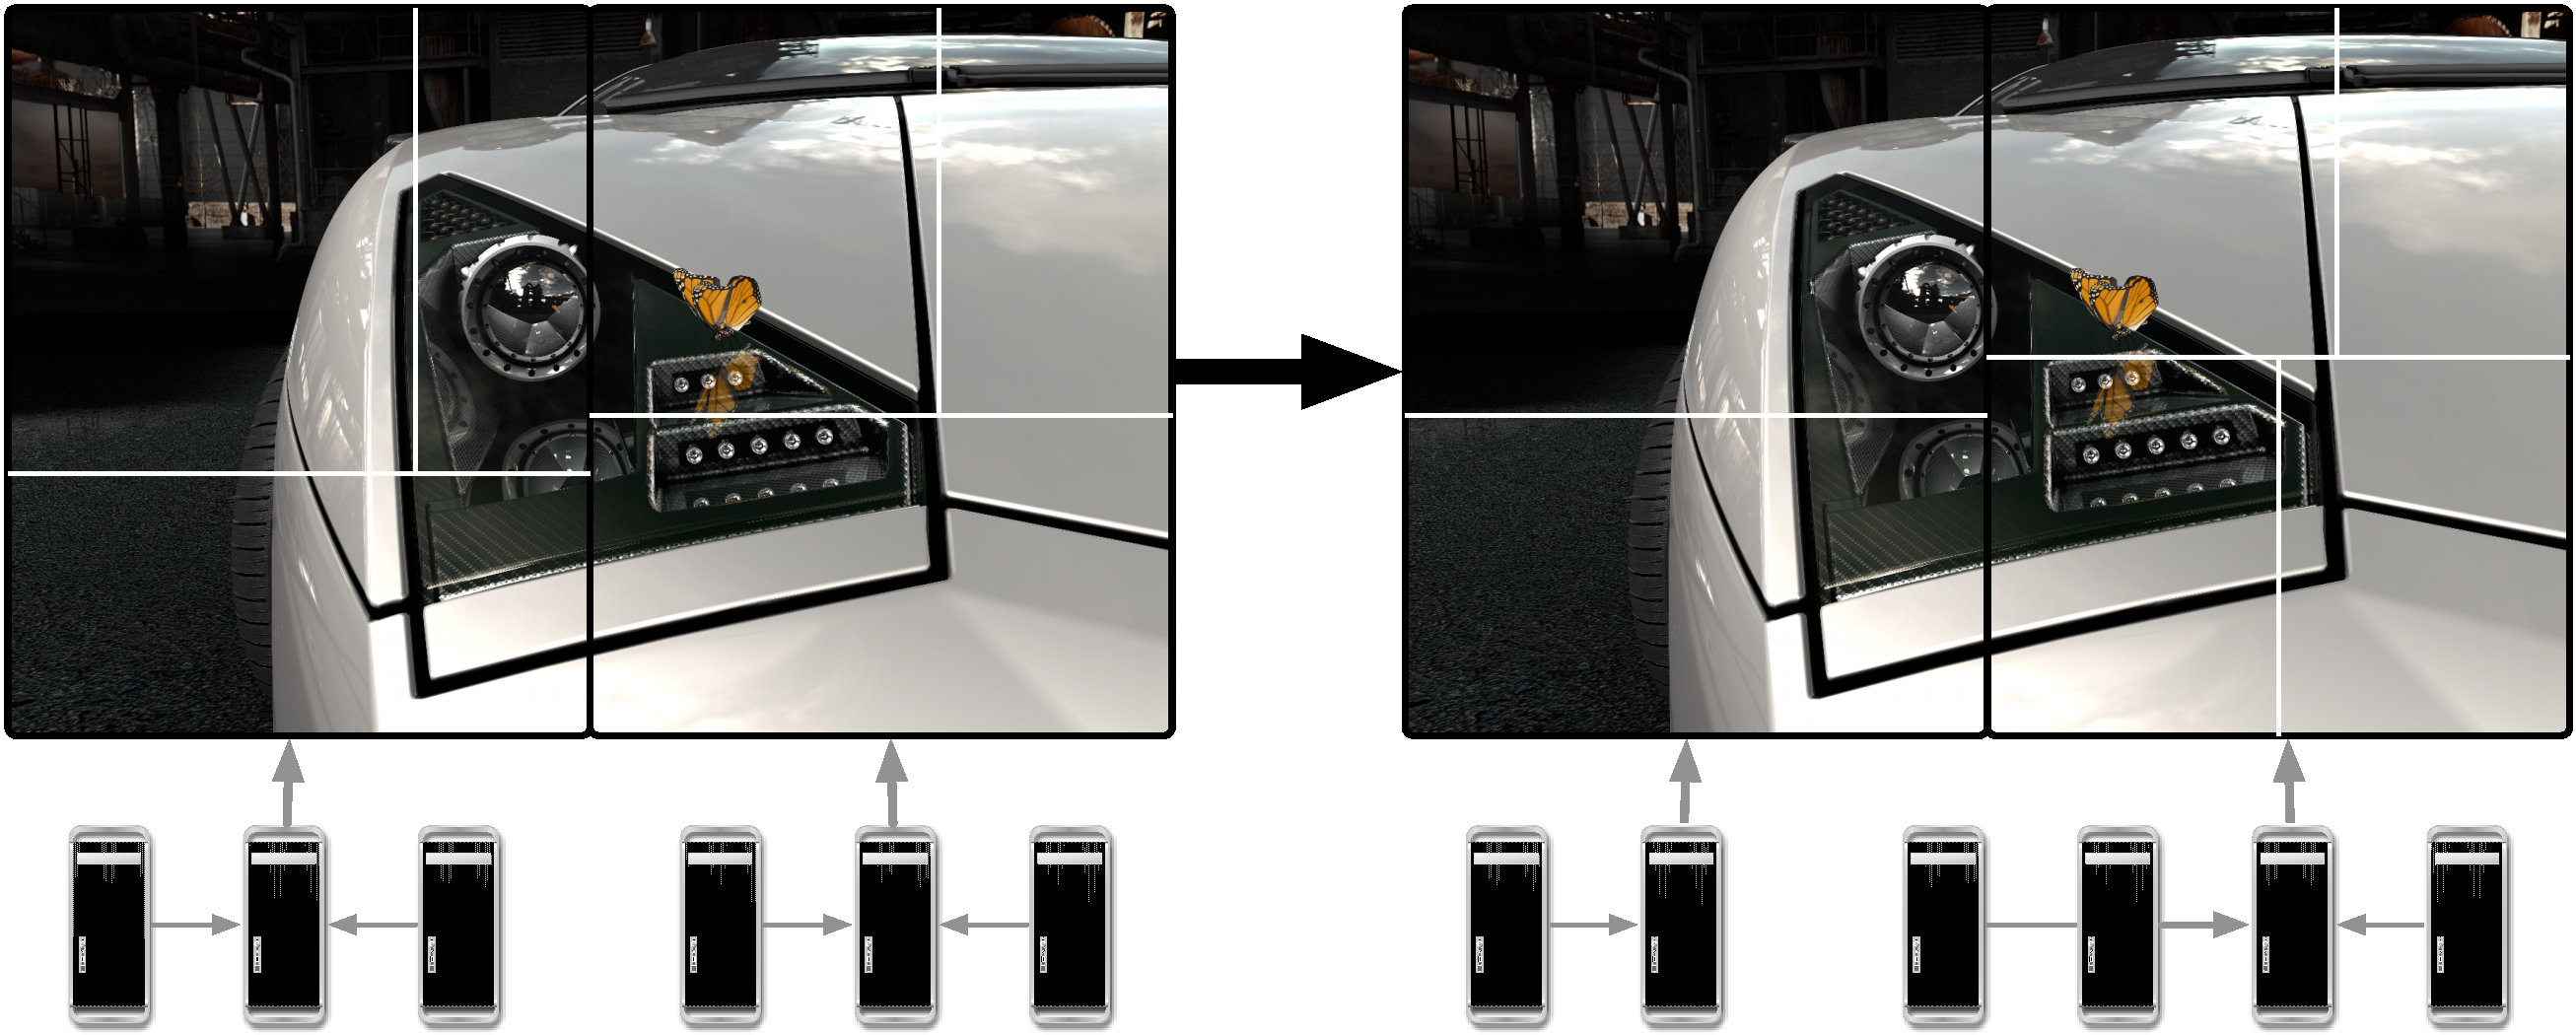
\includegraphics[width=.618\textwidth]{images/viewLB.pdf}
  {\caption{\label{fViewLoadBalancing}\small Cross-Segment
      Load-Balancing for two Segments using eight GPUs}}
\end{wrapfigure}
\fig{fViewLoadBalancing}\footnote{Image Copyright Realtime Technology
  AG, 2008} illustrates this process. On the left side, a static
assignment of resources to display segments is used. The right-hand
segment has a higher load than the left-hand segment, causing
sub-optimal performance. The configuration on the right uses a view
equalizer, which assigns two GPUs to the left segment and four GPUs to
the right segment, which leads to optimal performance for this model and
camera position.

The view equalizer can also use resources from another display resource,
if this resource has little rendering load by itself. It is therefore
possible to improve the rendering performance of a multi-display system
without any additional resources. This is particularly useful for
installations with a higher number of displays where the rendering load
is typically in a few segments only, e.g., for a CAVE.

\begin{wrapfigure}{l}{.382\textwidth}
    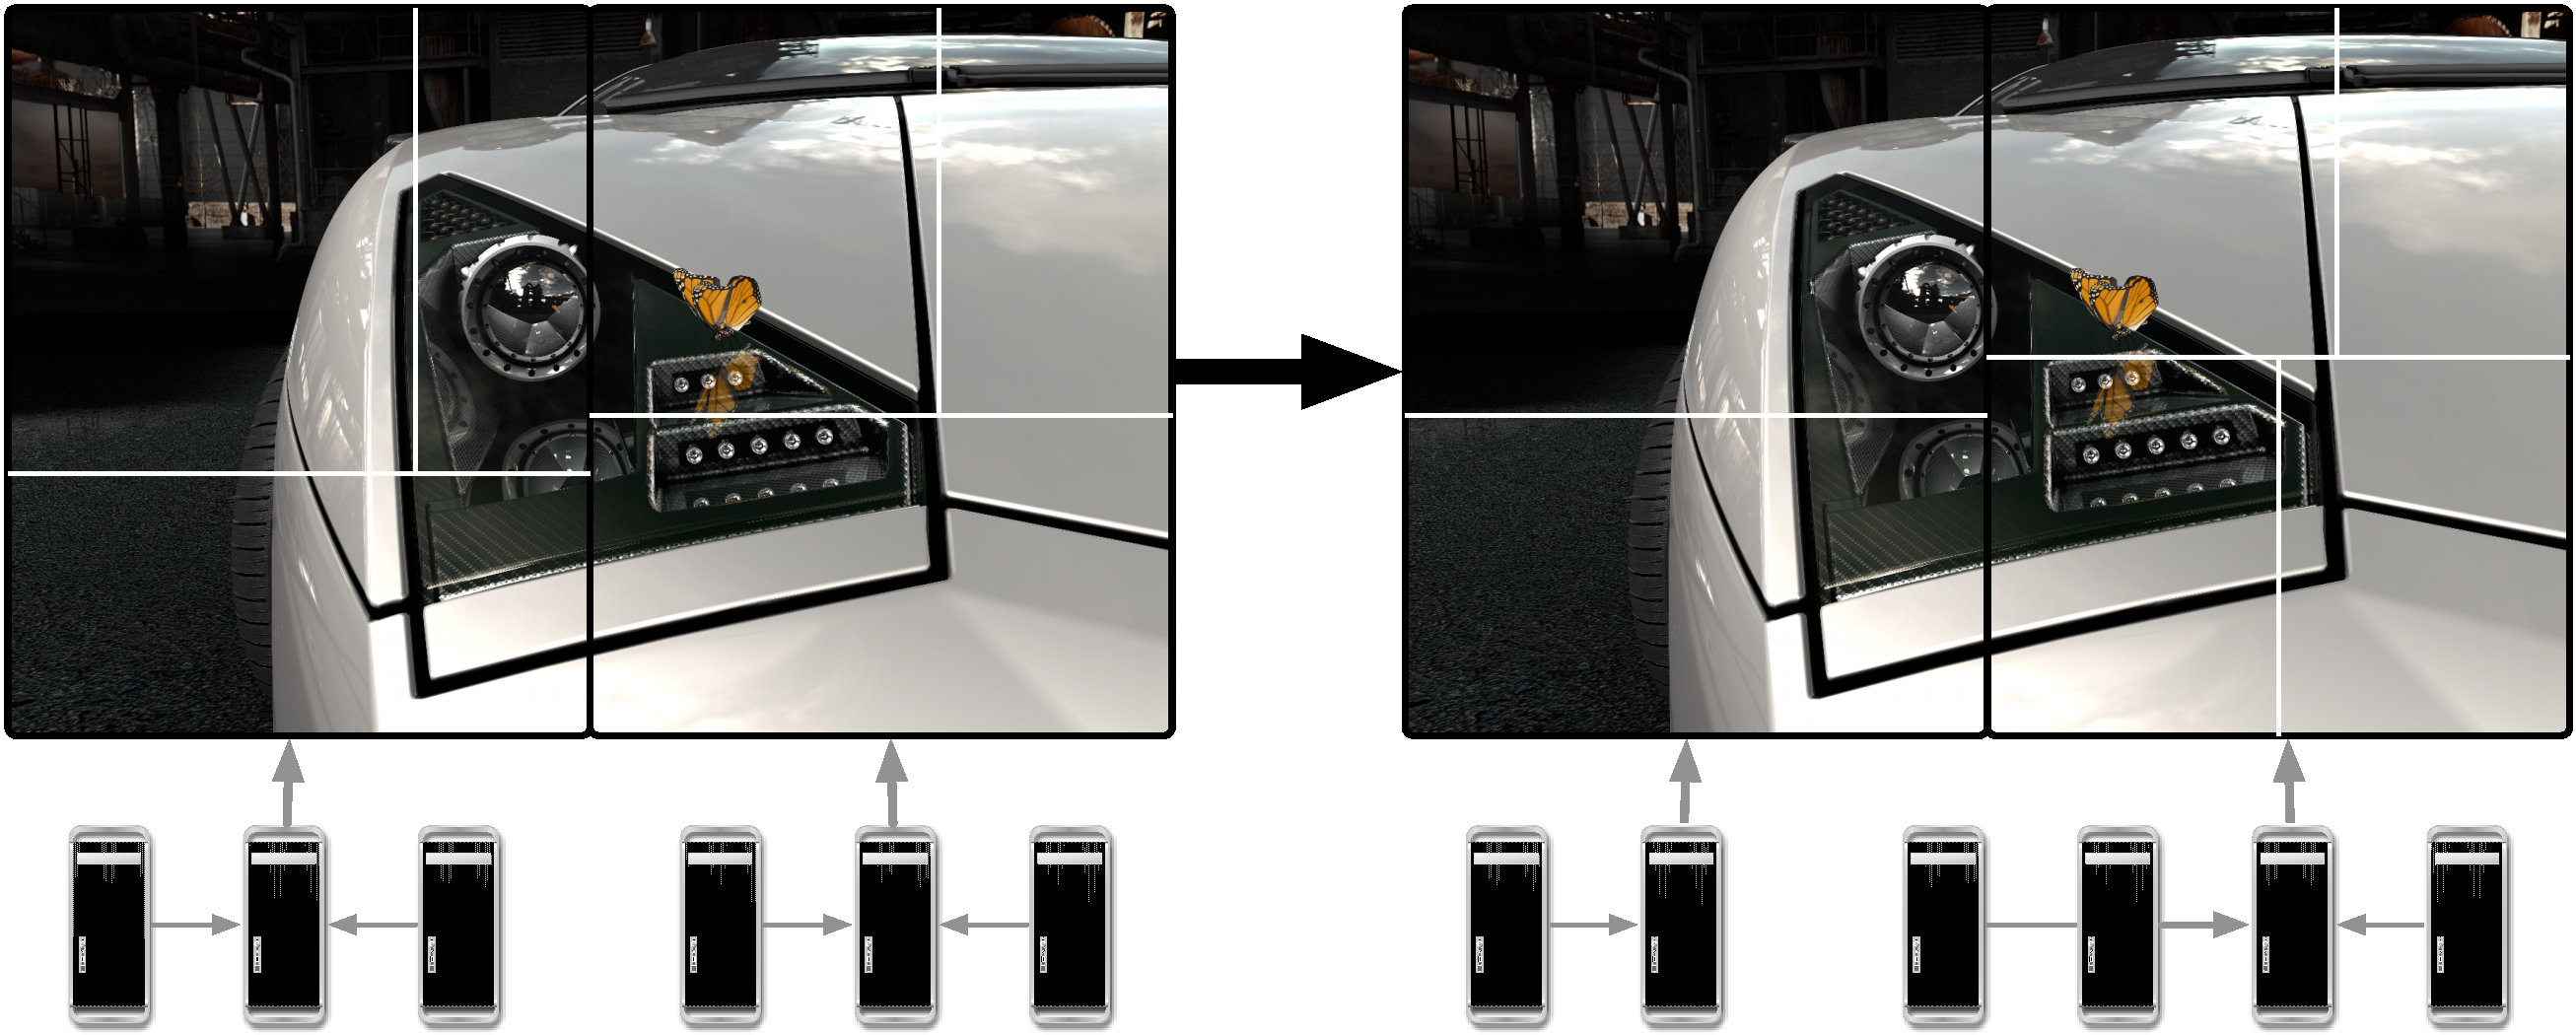
\includegraphics[width=.382\textwidth]{images/viewLB.png}
    {\caption{\label{fViewLoadBalancing2}\small Cross-Segment
        Load-Balancing for a CAVE}}
\end{wrapfigure}
\fig{fViewLoadBalancing2} shows cross-usage for a five-sided CAVE driven
by five GPUs. The front and left segments show the model and have a
significant rendering load. The view equalizer assigns the GPUs from
the top, bottom and right wall for rendering the left and front wall in
this configuration.

Cross-segment load-balan\-cing is configured hierarchically. On the top
compound level, a view equalizer assigns resources to each of its
children, so that the optimal number of resources is used for each
segment. On the next level, a load equalizer on each child computes the
resource distribution within the segment, taking the resource usage
given by the view equalizer into account.

\paragraph{Framerate Equalizer}
Certain configurations, in particular DPlex compounds, require a
smoothing of the framerate at the destination channel, otherwise the
framerate will become periodically faster and slower. Using a framerate
equalizer will smoothen the swap buffer rate on the destination window
for optimal user experience.

\paragraph{DFR Equalizer}

Dynamic Frame Resolution (DFR) trades rendering performance for visual
quality. The rendering for a channel is done at a different resolution
than the native channel resolution to keep the framerate constant. The
DFR equalizer adjusts the zoom of a channel, based on the target and
current framerate. It is typically used for fill-rate bound
applications, such as volume rendering and ray-tracing.

\begin{wrapfigure}{r}{.618\textwidth}
  \includegraphics[width=.618\textwidth]{images/dfr.pdf}
  {\caption{\label{fDFR}Dynamic Frame Resolution}}
\end{wrapfigure}
\fig{fDFR}\footnote{Data set courtesy of Olaf Ronneberger, Computer
  Science Institute, University of Freiburg, Germany} shows DFR for
volume rendering. To achieve 10 frames per second, the model is rendered
at a lower resolution, and upscaled to the native resolution for
display. The rendering quality is slightly degraded, while the rendering
performance remains interactive. When the application is idle, it
renders a full-resolution view.

The dynamic frame resolution is not limited to subsampling the rendering
resolution, it will also supersample the image if the source buffer is big
enough. Upscaled rendering, which will down-sample the result for display,
provides dynamic anti-aliasing at a constant framerate.

\paragraph{Monitor Equalizer}
The monitor equalizer allows the observation of another view,
potentially made of multiple segments, in a different channel at a
different resolution. This is typically used to reuse the rendering of
a large-scale display on an operator station.

\begin{wrapfigure}{r}{.618\textwidth}
  \includegraphics[width=.618\textwidth]{images/monitorEq.pdf}
  {\caption{\label{fMonitorEq}Monitoring a Projection Wall}}
\end{wrapfigure}
A monitor equalizer adjusts the frame zoom of the output frames used to
observe the rendering, depending on the destination channel size. The
output frames are downscaled on the GPU before readback, which results
in optimal performance.

\fig{fMonitorEq} shows a usage of the monitor equalizer. A two-segment
display wall is driven by a separate control station. The rendering
happens only on the display wall, and the control window receives the
correctly downscaled version of the rendering.


\section{\label{sClusterSetup}Setting up a Visualization Cluster}
This section covers the setup of a visualization cluster to run Equalizer
applications. It does not cover basic cluster management and driver
installation. A prerequisite to the following steps is a preinstalled cluster,
including network and graphics card drivers.

\subsection{Name Resolution}
Pay attention that your name resolution works properly, that is, the output of
the hostname command should resolve to the same, non-local IP address on all
machines. If this is not the case, you will have to provide the public IP
address for all processes, in the following way:
\begin{description}
\item[Server] Specify the server IP as the hostname field in the connection
  description in the server section.
\item[Application] Specify the application IP as the hostname field in the
  connection description in the appNode section. If the application should not
  contribute to the rendering, set up an appNode without a pipe section.
\item[Render Clients] Specify the client IPs as the hostname field in the
  connection description of each node section.
\end{description}

\subsection{Server}
The server may be started as a separate process or within the application
process. If it is started separately, simply provide the desired configuration
file as a parameter. It will listen on all network addresses, unless other
connection parameters are specified in the configuration file. If the
server is started within the application process, using the \textsf{--eq-config}
parameter, you will have to specify a connection description for the server in
the configuration file. Application-local servers do not create a listening
socket by default for security reasons.

\subsection{Starting Render Clients}
Cluster configurations use multiple Equalizer nodes, where each node represents
a separate process, typically on a different machine. These node processes have
to be started for a visualization session, and need to communicate with each
other.

Equalizer supports prelaunched render clients and automatic render client
launching, if configured properly. Prelaunched render clients are started
manually or by an external script on a predefined address. Auto-launched render
client are started and stopped by the Equalizer server on demand.

The two mechanism can coexist. The server will first try to connect a
prelaunched render client on the given connection descriptions for each
node. If this fails, he will try to auto-launch the render client. If the render
client does not connect back to the server within a certain timeout (default one
minute), a failure to initialize the configuration is reported back to the
application.

\subsubsection{\label{sResident}Prelaunched Render Clients}
Prelaunched render clients are useful if setting up auto-launching is too
time-consuming, e.g., on Windows which does not have a standard remote login
procedure. The following steps are to be taken to use prelaunched render
clients:

\begin{itemize}
\item Set the \textbf{connection} hostname and port parameters of each node in
  the configuration file.
\item Start the \textbf{render clients} using the parameters
  \textsf{--eq-client} and \textsf{--eq-listen}, e.g.,
  \textsf{./build/Linux/bin/eqPly --eq-client --eq-listen
  192.168.0.2:1234}. Pay attention to use the same connection parameters as in
    the configuration file.
\item Start the \textbf{application}. If the server is running on the same
  machine and user as the application, the application will connect to it
  automatically. Otherwise use the \textsf{--eq-server} parameter to specify the
  server address.
\end{itemize}

The render clients will automatically exit when the config is closed. The
\textsf{eqPly} example application implements the option \textsf{-r} to keep the
render client processes resident.

\subsubsection{Auto-launched Render Clients}
To automatically launch the render clients, the server needs to know the name of
the render client and the command to launch them without user interaction.

The name of the render client is automatically set to the name of the
application executable. This may be changed programmatically by the
application. Normally it suffices to install the application in the same
directory on all machines, ideally using a shared file system.

The default launch command is set to ssh, which is the most common solution for
remote logins. To allow the server to launch the render clients without user
interaction, password-less ssh needs to be set up. Please refer to the ssh
documentation (cf. \textsf{ssh-keygen} and \textsf{~/.ssh/authorised\_keys}) and
verify the functionality by logging in to each machine from the host running the
server.

\subsection{Debugging}
If your configuration does not work, simplify it as much as possible
first. Normally this means that there is one server, application and render
client. Failure to launch a cluster configuration often is caused by one of the
following reasons:
\begin{itemize}
\item A firewall is blocking network connections.
\item The render client can't access the GPUs on the remote host. Set up your
  X-Server or application rights correctly. Log into the remote machine using
  the launch command and try to execute a simple application, e.g.,
  \textsf{glxinfo -display :0.1}.
\item The server does not find the prelaunched render client. Verify that the
  client is listening on the correct IP and port, and that this IP and port are
  reachable from the server host.
\item The server cannot launch a render client. Check the server log for the
  launch command used, and try to execute a simple application from the server
  host using this launch command. It should run without user interaction. Check
  that the render client is installed in the correct path. Pay attention to the
  launch command quotes used to separate arguments on Windows. Check that the
  same software versions, including Equalizer, are installed on all machines.
\item A client can't connect back to the application. Check the client log, this
  is typically caused by a misconfigured host name resolution.
\end{itemize}

\clearpage
\part{Programming Guide}

To modify an application for Equalizer, the programmer structures the
source code so that the OpenGL rendering can be executed in parallel,
potentially using multiple processes for cluster-based execution.

\section{\label{sHello}Hello, World!}

The \textsf{eqHello} example is a minimal application to illustrate the basic
principle of any Equalizer application: The application developer has to
implement a rendering method similar to the \textsf{glutDisplayFunc} in GLUT
applications.

\begin{wrapfigure}{r}{.618\textwidth}
  \includegraphics[width=.618\textwidth]{images/eqHello.png}
  {\caption{\label{fHello}Hello, World!}}
\end{wrapfigure}
It can be run as a stand-alone application from the command line or using an
explicit configuration file for a visualization cluster. In the stand-alone
case, any Equalizer application, including eqHello, will automatically configure
itself to use all graphics cards found on the local system for scalability.

The \textsf{eqHello} example uses Sequel, a thin layer on top of the canonical
Equalizer programming interface. \sref{sSeqPly} introduces Sequel in detail, and
\sref{sEqPly} introduces the full scope of the Equalizer API.

The main \textsf{eqHello} function instantiates an application object,
initializes it, starts the main loop and finally de-initializes the application:

{\footnotesize\lstinputlisting[firstline=56, lastline=64]
  {../../../Equalizer/examples/eqHello/hello.cpp}}

The application object represents one process in the cluster. The primary
application instance has the rendering loop and controls all execution. All
other instances used for render client processes are passive and driven by
Equalizer. The application is responsible for creating the renderers, of which
one per GPU is used:

{\footnotesize\lstinputlisting[firstline=47, lastline=53]
  {../../../Equalizer/examples/eqHello/hello.cpp}}

The renderer is responsible for executing the application's rendering code. One
instance for each GPU is used. All calls to a single renderer are executed
serially and therefore thread-safe.

In \textsf{eqHello}, the renderer draws six colored quads. The only change from
a standard OpenGL application is the usage of the rendering context provided by
Equalizer, most notably the frustum and viewport. The rendering context is
described in detail in \sref{sRenderContext}, and \textsf{eqHello} simply calls
\textsf{applyRenderContext} which will execute the appropriate OpenGL calls.

After setting up lighting, the model is positioned using
\textsf{applyModelMatrix}. For convenience, Sequel maintains one camera per
view. The usage of this camera is purely optional, an application can implement
its own camera model.

The actual OpenGL code, rendering six colored quads, is omitted here for
brevity:

{\footnotesize\lstinputlisting[firstline=67, lastline=79]
  {../../../Equalizer/examples/eqHello/hello.cpp}}


\section{Programming Interface}

Equalizer uses a C++ programming interface. The API is minimally
invasive. Equalizer imposes only a minimal, natural execution framework upon the
application. It does not provide a scene graph, or interferes in any other way
with the application's rendering code. The restructuring work enforced by
Equalizer is the minimal refactoring needed to parallelize the application for
scalable, distributed rendering.

The API documentation is available on the website or in the header files, and
provides a comprehensive documentation on individual methods, types and other
elements of the API. Methods marked with a specific version are part of the
official, public API and have been introduced by this Equalizer
version. Reasonable care is taken to not break API compatibility or change the
semantics of these methods within future Equalizer versions of the same major
revision. Any eventual changes to the public API are documented in the release
notes and the file \textsf{CHANGES.txt}.

In addition the official, public API Equalizer exposes a number of
unstable methods and, where unavoidable, internal APIs. These are clearly marked
in the API documentation. Unstable methods may be used by the programmer, but
their interface or functionality may change in any future Equalizer version. The
usage of internal methods is discouraged. Undocumented or unversioned methods
should be considered as part of the unstable API.

\subsection{\label{sNamespaces}Namespaces}

The Equalizer software stack is modularized, layering gradually more powerful,
but less generic APIs on to of each other. It furthermore relies on a number of
required and optional libraries. Application developers are exposed to the
following name\-spa\-ces:

\begin{description}
\item[seq] The core namespace for Sequel, the simple interface to the Equalizer
  client library.
\item[eq] The core namespace for the Equalizer client library. The classes and
  their relationship in this namespace closely model the configuration file
  format. The classes in the \textsf{eq} namespace are the main subject of this
  Programming Guide.\fig{fClientUml} provides an overview map of the most
  important classes in the Equalizer namespace, grouped by functionality.
\item[eq::util] The eq::util namespace provides common utility classes, which
  often simplify the usage of OpenGL functions. Most classes in this namespace
  are used by the Equalizer client library, but are usable independently
  from Equalizer for application development.
\item[eq::admin] The eq::admin namespace implements an administrative API to
  change the configurations of a running server. This admin API is not yet
  finalized and will very likely change in the future.
\item[eq::fabric] The eq::fabric namespace is the common data management and
  transport layer between the client library, the server and the administrative
  API. Most Equalizer client classes inherit from base classes in this namespace
  and have all their data access methods in these base classes.
\item[co] Collage is the network library used by Equalizer. It provides basic
  functionality for network communication, such as \textsf{Connection} and
  \textsf{ConnectionSet}, as well as higher-level functionality such as
  \textsf{Node}, \textsf{LocalNode}, \textsf{Object} and
  \textsf{Serializable}. Please refer to \sref{sNetwork} for an introduction
  into the network layer, and to \sref{sNetObject} for distributed objects.
\item[lunchbox] The lunchbox library provides C++ classes to abstract the
  underlying operating system and to implement common helper functionality for
  multi-threaded applications. Examples are \textsf{lunchbox::Clock} providing a
  high-resolution timer, or \textsf{lunchbox::MTQueue} providing a thread-safe,
  blocking FIFO. Classes in this namespace are fully documented in the API
  documentation on the Equalizer website, and are not subject of this
  Programming Guide.
\item[hwloc, boost, vmmlib, hwsd] External libraries providing manual and
  automatic thread affinity, serialization and the foundation for RSP multicast,
  vector and matrix mathematics as well as local and remote hardware (GPU,
  network interfaces) discovery, respectively. The hwloc and hwsd libraries are
  used only internally and not exposed through the API.
\item[eq::server] The server namespace, implementing the functionality of the
  Equalizer server, which is an internal namespace not to be used by application
  developers. The \textsf{eq::admin} namespace enables run-time administration
  of Equalizer servers. The server does not yet expose a stable
  API.
\end{description}

\begin{wrapfigure}{r}{.618\textwidth}
  \includegraphics[width=.618\textwidth]{images/namespaces} % TODO: update image (hwsd)
  {\caption{\label{fNamespaces}Namespaces}}
\end{wrapfigure}
The Equalizer examples are implemented in their own namespaces, e.g.,
\textsf{eqPly} or \textsf{eVolve}. They rely mostly on subclassing from the
\textsf{eq} namespace, with the occasional usage of functionality from the
\textsf{eq::util}, \textsf{eq::fabric}, \textsf{co} and \textsf{lunchbox}
namespace. \fig{fNamespaces} shows the namespaces and their layering.

\begin{figure}[ht!]\center
  \includegraphics[width=\textwidth]{images/clientUML}
  {\caption{\label{fClientUml}Equalizer client UML map}}
\end{figure}

\subsection{\label{sTaskMethods}Task Methods}

Methods called by the application have the form \textsf{verb[Noun]},
whereas methods called by Equalizer (`Task Methods') have the form
\textsf{nounVerb}. For example, the application calls
\textsf{Config::startFrame} to render a new frame, which causes, among
many other things, \textsf{Node::frameStart} to be called in all active
render clients.

The application inherits from Equalizer classes and overrides virtual
functions to implement certain functionality, e.g., the application's
OpenGL rendering in \textsf{eq::Chan\-nel::frameDraw}. These task
methods are similar in concept to C function callbacks. \sref{sEqPly}
will discuss the important task methods. A full list can be found on the
website\footnote{see
  \link{http://www.equalizergraphics.com/documents/design/taskMethods.html}}.

\subsection{\label{sExecution}Execution Model and Thread Safety}

Using threading correctly in OpenGL-based applications is easy with
Equalizer. Equalizer creates one rendering thread for each graphics
card. All task methods for a pipe, and therefore all OpenGL commands,
are executed from this thread. This threading model follows the OpenGL
`threading model', which maintains a current context for each
thread. If structured correctly, the application rarely has to take care
of thread synchronization or protection of shared data.

The main thread is responsible for maintaining the application logic. It
reacts on user events, updates the data model and requests new frames to
be rendered. It drives the whole application, as shown in \fig{fModel}.

\begin{wrapfigure}{r}{.618\textwidth}
  \includegraphics[width=.618\textwidth]{images/model.pdf}
  {\caption{\label{fModel}Simplified Execution Model}}
\end{wrapfigure}
The rendering threads concurrently render the application's
database. The data\-base should be accessed in a read-only fashion
during rendering to avoid threading problems. This is normally the case,
for example all modern scene graphs use read-only render traversals, writing the
GPU-specific information into a separate per-GPU data structure.

All rendering threads in the configuration run asynchronously to the
application's main thread. Depending on the configuration's latency,
they can fall $n$ frames behind the last frame finished by the
application thread. A latency of one frame is usually not perceived by
the user, but can increase rendering performance substantially since
operations can be better pipelined.

Rendering threads on a single node are synchronized when using the
default thread model \textsf{draw\_sync}. When a frame is finished, all
local rendering threads are done drawing. Therefore the application can
safely modify the data between the end of a frame and the beginning of a
new frame. Furthermore, only one instance of the scene data has to be
maintained within a process, since all rendering threads are guaranteed
to draw the same frame.

This per-node frame synchronization does not inhibit latency across rendering
nodes. Furthermore, advanced rendering software which multi-buffers the dynamic
parts of the database can disable the per-node frame synchronization, as
explained in \sref{sThreadModel}. Some scene graphs implement multi-buffered
data, and can profit from relaxing the local frame synchronization.



\section{\label{sSeqPly}Sequel: The seqPly Polygonal Renderer}

In this section the source code of \textsf{seqPly} is used to introduce the
Sequel API in detail, and relevant design decisions, caveats and other remarks
are discussed. Sequel is conceived to lower the entry barrier into creating
parallel rendering applications without sacrificing major functionality. It
implements proven design patterns of Equalizer applications. Sequel does not
prohibit the usage of Equalizer or Collage functionality, it simply makes it
easier to use for the common use cases.

The \textsf{seqPly} parallel renderer provides a subset of features found in its
cousin application, \textsf{eqPly}, introduced in the next section. It is more
approachable, using approximately one tenth of the source code needed by
\textsf{eqPly} due to the use of the Sequel abstraction layer and reduced
functionality.


\subsection{main Function}

The main function is almost identical to \textsf{eqHello}. It instantiates an
application object, initializes it, starts the main loop and finally
de-initializes the application. The source code is not reproduced here due to
its similarity with \sref{sHello}.

\subsection{Application}

The application object in Sequel represents one process in the cluster. The main
application instance has the rendering loop and controls all execution. All
other instances used for render client processes are passive and driven by
Equalizer.

Sequel applications derive their application object from
\textsf{seq::Application} and selectively override functionality. They have to
implement \textsf{createRenderer}, as explained below. The \textsf{seqPly}
application overrides init, exit, run and implements createRenderer.

The initialization and exit routines are overwritten to parse
\textsf{seqPly}-specific command line options and to load and unload the
requested model:

{\footnotesize\lstinputlisting[firstline=41, lastline=49]
  {../../../Equalizer/examples/seqPly/application.cpp}}
{\footnotesize\lstinputlisting[firstline=56, lastline=60]
  {../../../Equalizer/examples/seqPly/application.cpp}}

Sequel manages distributed objects, simplifying their use. This includes
registration, automatic creation and mapping as well as commit and
synchronization of objects. One special object for initialization (not used in
\textsf{seqPly}) and one for per-frame data are managed by Sequel, in addition
to an arbitrary number of application-specific objects.

The objects passed to \textsf{seq::Application::init} and
\textsf{seq::Application::run} are automatically distributed and instantiated on
the render clients, and then passed to the respective task callback methods. The
application may pass a 0 pointer if it does not need an object for
initialization or per-frame data. Objects are registered with a type, and when
automatically created, the \textsf{createObject} method on the application or
renderer is used to create an instance based on this type.

The run method is overloaded to pass the frame data object to the Sequel
application run loop. The object will be distributed and synchronized to all
renderers:

{\footnotesize\lstinputlisting[firstline=51, lastline=55]
  {../../../Equalizer/examples/seqPly/application.cpp}}

The application is responsible for creating renderers. Sequel will request one
renderer for each GPU rendering thread. Sequel also provides automatic mapping
and synchronization of distributed objects, for which the application has to
provide a creation callback:

{\footnotesize\lstinputlisting[firstline=62, lastline=77]
  {../../../Equalizer/examples/seqPly/application.cpp}}


\subsection{Renderer}

The renderer is responsible for executing the application's rendering code. One
instance for each GPU is used. All calls to a single renderer are executed
serially and therefore thread-safe.

The \textsf{seqPly} rendering code uses the same data structure and algorithm as
\textsf{eqPly}, described in \sref{sRendering}. This renderer captures the
GPU-specific data in a \textsf{State} object, which is created and destroyed
during init and exit. The state captures also the OpenGL function table, which
is available when init is called, but not yet during the constructor of the
renderer:

{\footnotesize\lstinputlisting[firstline=46, lastline=59]
  {../../../Equalizer/examples/seqPly/renderer.cpp}}

The rendering code is similar to the typical OpenGL rendering code, except for a
few modifications to configure the rendering. First, the render context is
applied and lighting is set up. The render context, described in detail in
\sref{sRenderContext}, sets up the stereo buffer, 3D viewport as well as the
projection and view matrices using the appropriate OpenGL calls. Applications
can also retrieve the render context and apply the settings themselves:

{\footnotesize\lstinputlisting[firstline=69, lastline=80]
  {../../../Equalizer/examples/seqPly/renderer.cpp}}

After the static light setup, the model matrix is applied to the existing view
matrix, completing the modelview matrix and positioning the model. Sequel
maintains a per-view camera, which is modified through mouse and keyboard events
and determines the model matrix. Applications can overwrite this event handling
and maintain their own camera model. Afterwards, the state is set up with the
projection-modelview matrix for view frustum culling, the DB range for sort-last
rendering and the cull-draw traversal is executed, as described in
\sref{sRendering}:

{\footnotesize\lstinputlisting[firstline=81, lastline=97]
  {../../../Equalizer/examples/seqPly/renderer.cpp}}


\section{\label{sEqPly}Equalizer: The eqPly Polygonal Renderer}

In this section the source code of \textsf{eqPly} is used to introduce the
Equalizer API in detail, and relevant design decisions, caveats and other
remarks are discussed.

\textsf{eqPly} is a parallel renderer for polygonal data in the
\textsf{ply} file format. It supports all relevant Equalizer features,
and can be used to render on large-scale displays, immersive
environments with head tracking and to render massive data sets using
all scalable rendering features of Equalizer. It is a superset of
\textsf{seqPly}, introduced in \sref{sSeqPly}.

The \textsf{eqPly} example is shipped with the Equalizer distribution
and serves as a reference implementation of an Equalizer-based
application of medium complexity. It focuses on the example usage of
core Equalizer features, not on advanced rendering features or visual
quality.

\begin{figure}[ht!]\center
  \includegraphics[width=.9\textwidth]{images/uml}
  {\caption{\label{fUml}UML Diagram eqPly and relevant Equalizer Classes}}
\end{figure}

\fig{fUml} shows how the most important Equalizer classes are used through
inheritance by the \textsf{eqPly} example. All classes in the example are in the
\textsf{eqPly} namespace to avoid type name ambiguities, in particular for the
\textsf{Window} class which is frequently used as a type in the global namespace
by windowing systems.

The \textsf{eqPly} classes fall into two categories: Subclasses of the
rendering entities introduced in \sref{sConfig}, and classes for
distributing data.

The function and typical usage for each of the rendering entities is discussed
in this section. Each of these classes inherits from a base class in the
\textsf{eq::fabric} name\-space, which implements data distribution for the
entity. The fabric base classes are omitted in \fig{fUml}.

The distributed data classes are helper classes based on
\textsf{co::Serializable} or its base class \textsf{co::Object}. They illustrate
the typical usage of distributed objects for static as well as dynamic,
frame-specific data. Furthermore they are used for a basic scene graph
distribution of the model data to the render client processes.


\subsection{main Function}

The main function starts off with initializing the Equalizer library. The
command line arguments are passed on to Equalizer. They are used to set certain
default values based on Equalizer-specific options\footnote{Equalizer-specific
  options always start with -\,-eq-}, e.g., the default server
address. Furthermore, a \textsf{NodeFactory} is provided. The \textsf{EQERROR}
macro, and its counterparts \textsf{EQWARN}, \textsf{EQINFO} and \textsf{EQVERB}
allow selective debugging outputs with various logging levels:

{\footnotesize\lstinputlisting[firstline=58, lastline=68]
  {../../../Equalizer/examples/eqPly/main.cpp}}

The node factory is used by Equalizer to create the object instances of
the configured rendering entities. Each of the classes inherits from the
same type provided by Equalizer in the \textsf{eq} namespace. The
provided \textsf{eq::NodeFactory} base class instantiates 'plain'
Equalizer objects, thus making it possible to selectively subclass
individual entity types, as it is done by \textsf{eqHello}. For each
rendering resources used in the configuration, one C++ object will be
created during initialization. Config, node and pipe objects are created and
destroyed in the node thread, whereas window and channel objects are
created and destroyed in the pipe thread:

{\footnotesize\lstinputlisting[firstline=40, lastline=57]
  {../../../Equalizer/examples/eqPly/main.cpp}}

The second step is to parse the command line into the
\textsf{LocalInitData} data structure. A part of it, the base class
\textsf{InitData}, will be distributed to all render client nodes. The
command line parsing is done by the \textsf{LocalInitData} class, which
is discussed in \sref{sInitData}:

{\footnotesize\lstinputlisting[firstline=70, lastline=73]
  {../../../Equalizer/examples/eqPly/main.cpp}}

The third step is to create an instance of the application and to initialize it
locally. The application is a subclass of \textsf{eq::Client}, which in turn is
an \textsf{co::LocalNode}. The underlying Collage network library, discussed in
\sref{sNetwork}, is a peer-to-peer network of \textsf{co::LocalNode}s. The
client-server concept is implement the higher-level \textsf{eq} client
namespace.

The local initialization of a node creates at least one local listening socket,
which allows the \textsf{eq::Client} to communicate over the network with other
nodes, such as the server and the rendering clients. The listening socket(s) can
be configured using the \textsf{--eq-listen} command line parameter, by adding
connections to the \textsf{appNode} in the configuration file, or by
programmatically adding connection descriptions to the client before the local
initialization:

{\footnotesize\lstinputlisting[firstline=74, lastline=81]
  {../../../Equalizer/examples/eqPly/main.cpp}}

Finally everything is set up, and the \textsf{eqPly} application is executed:

{\footnotesize\lstinputlisting[firstline=83, lastline=84]
  {../../../Equalizer/examples/eqPly/main.cpp}}

After the application has finished, it is de-initialized and the
\textsf{main} function returns:

{\footnotesize\lstinputlisting[firstline=85]
  {../../../Equalizer/examples/eqPly/main.cpp}}

\subsection{Application}

In the case of \textsf{eqPly}, the application is also the render
client. The \textsf{eqPly} executable has three runtime behaviors:

\begin{enumerate}
\item \textbf{Application}: The executable started by the user, the
  controlling entity of the rendering session.
\item \textbf{Auto-launched render client}: The typical render client,
  started by the server. The server starts the executable with special
  parameters, which cause \textsf{Client::initLocal} to never
  return. During exit, the server terminates the process. By default,
  the server starts the render client using \textsf{ssh}. The launch
  command can be used to configure another program to auto-launch render
  clients.
\item \textbf{Resident render client}: Manually prestarted render
  client, listening on a specified port for server commands. This mode
  is selected using the command-line option \textsf{--eq-client} and
  \textsf{--eq-listen \textless address\textgreater} to specify a
  well-defined listening address, and potentially \textsf{-r} to keep
  the client running across multiple runs\footnote{see
    \link{http://www.equalizergraphics.com/documents/design/residentNodes.html}}.
\end{enumerate}

\subsubsection{Main Loop}

The application's main loop starts by connecting the application to an Equalizer
server. If no server is specified, \textsf{Client::connectServer} tries first to
connect to a server on the local machine using the default port. If that fails,
it will create a server running within the application process using
auto-configuration as described in \sref{sHWSDUsage}. The command line
parameter \textsf{--eq-config} can be used to specify a hwsd session or
configuration file, and \textsf{--eq-server} to explicitly specify a server
address.

{\footnotesize\lstinputlisting[firstline=83, lastline=91]
  {../../../Equalizer/examples/eqPly/eqPly.cpp}}

The second step is to ask the server for a configuration. The
\textsf{ConfigParams} are a placeholder for later Equalizer implementations to
provide additional hints and information to the server for
auto-configuration. The configuration chosen by the server is created locally
using \textsf{NodeFactory::createConfig}. Therefore it is of type
\textsf{eqPly::Config}, but the return value is \textsf{eq::Config}, making the
static\_cast necessary:

{\footnotesize\lstinputlisting[firstline=93, lastline=103]
  {../../../Equalizer/examples/eqPly/eqPly.cpp}}

Finally it is time to initialize the configuration. For statistics, the
time for this operation is measured and printed. During initialization
the server launches and connects all render client nodes, and calls the
appropriate initialization task methods, as explained in later
sections. \textsf{Config::init} returns after all nodes, pipes,
windows and channels are initialized.

The return value of \textsf{Config::init} depends on the configuration
robustness attribute. This attribute is set by default, allowing configurations
to launch even when some entities failed to initialize. If set,
\textsf{Config::init} always returns true. If deactivated, it returns
\textsf{true} only if all initialization task methods were successful. In any
case, \textsf{Config::getError} only returns \textsf{ERROR\_NONE} if all
entities have initialized successfully.

The \textsf{EQLOG} macro allows topic-specific logging. The numeric
topic values are specified in the respective \textsf{log.h} header
files, and logging for various topics is enabled using the environment
variable \textsf{EQ\_LOG\_TOPICS}:

{\footnotesize\lstinputlisting[firstline=104, lastline=121]
  {../../../Equalizer/examples/eqPly/eqPly.cpp}}

When the configuration was successfully initialized, the main rendering
loop is executed. It runs until the user exits the
configuration, or when a maximum number of frames has been rendered,
specified by a command-line argument. The latter is useful for
benchmarks. The \textsf{Clock} is reused for measuring the overall
performance. A new frame is started using \textsf{Config::startFrame}
and a frame is finished using \textsf{Config::finishFrame}.

When a new frame is started, the server computes all rendering tasks and
sends them to the appropriate render client nodes. The render client
nodes dispatch the tasks to the correct node or pipe thread, where they
are executed in order of arrival.

\textsf{Config::finishFrame} blocks on the completion of the frame
\textsf{current - latency}. The latency is specified in the
configuration file, and allows several outstanding frames. This allows
overlapping execution in the node processes and pipe threads and
minimizes idle times.

By default, \textsf{Config::finish\-Fra\-me} also synchronizes the
completion of all local rendering tasks for the current frame. This
facilitates porting of existing rendering codes, since the database does
not have to be multi-buffered. Applications such as \textsf{eqPly}, which
do not need this per-node frame synchronization, can disable it as
explained in \sref{sThreadModel}:

{\footnotesize\lstinputlisting[firstline=123, lastline=134]
  {../../../Equalizer/examples/eqPly/eqPly.cpp}}

\fig{fSyncAsync} shows the execution of the rendering tasks of a 2-node 2D
compound without latency and with a latency of one frame. The asynchronous
execution pipelines certain rendering operations and hides imbalances in the
load distribution, resulting in an improved framerate. For example, we have
observed a speedup of 15\% on a five-node rendering cluster when using a latency
of one frame instead of no
latency\footnote{\link{http://www.equalizergraphics.com/scalability.html}}. A
latency of one or two frames is normally not perceived by the user. The
statistics overlay is explained in detail in \sref{sStatisticsOverlay}.

\begin{figure}[ht!]\center
  \includegraphics[width=\textwidth]{images/syncAsync}
  {\caption{\label{fSyncAsync}Synchronous and Asynchronous Execution}}
\end{figure}

When playing a camera animation, \textsf{eqPly} prints the rendering performance
once per animation loop for benchmarking purposes:

{\footnotesize\lstinputlisting[firstline=136, lastline=145]
  {../../../Equalizer/examples/eqPly/eqPly.cpp}}

\textsf{eqPly} uses event-driven execution, that is, it only request new
rendering frames if an event or animation requires an update. The
\textsf{eqPly::Config} maintains a dirty state, which is cleared after a
frame has been started, and set when an event causes a
redraw. Furthermore, when an animation is running or head tracking is
active, the config always signals the need for a new frame.

If the application detects that it is currently idle, all pending
commands are gradually flushed, while still looking for a redraw
event. Then it waits and handles one event at a time, until a redraw is
needed:

{\footnotesize\lstinputlisting[firstline=147, lastline=161]
  {../../../Equalizer/examples/eqPly/eqPly.cpp}}

When the main rendering loop has finished,
\textsf{Config::finishAllFrames} is called to catch up with the
latency. It returns after all outstanding frames have been rendered, and
is needed to provide an accurate measurement of the framerate:

{\footnotesize\lstinputlisting[firstline=163, lastline=167]
  {../../../Equalizer/examples/eqPly/eqPly.cpp}}

The remainder of the application code cleans up in the reverse order of
initialization. The config is exited, released and the connection to the server
is closed:

{\footnotesize\lstinputlisting[firstline=169, lastline=180]
  {../../../Equalizer/examples/eqPly/eqPly.cpp}}

\subsubsection{Render Clients}

In the second and third use case of the \textsf{eqPly}, when the
executable is used as a render client, \textsf{Client::initLocal} never
returns. Therefore the application's main loop is never executed. To
keep the client resident, the \textsf{eqPly} example overrides the
client loop to keep it running beyond one configuration run:

{\footnotesize\lstinputlisting[firstline=182, lastline=190]
  {../../../Equalizer/examples/eqPly/eqPly.cpp}}


\subsection{\label{sNetObject}Distributed Objects}

Equalizer provides distributed objects which facilitate the implementation of
data distribution in a cluster environment. Distributed objects are created by
subclassing from \textsf{co::Serializable} or \textsf{co::Object}. The
application programmer implements serialization and deserialization of the
distributed data. \sref{sNetObject2} covers distributed objects in detail.

Distributed objects can be static (immutable) or dynamic. Dynamic objects are
versioned. The \textsf{eqPly} example uses static distributed objects to provide
initial data and the model to all rendering nodes, as well as a versioned object
to provide frame-specific data such as the camera position to the rendering
methods.

\subsubsection{\label{sInitData}InitData - a Static Distributed Object}

The \textsf{InitData} class holds a couple of parameters needed during
initialization. These parameters never change during one configuration
run, and are therefore static.

On the application side, the class \textsf{LocalInitData} subclasses
\textsf{InitData} to provide the command line parsing and to set the
default values. The render nodes only instantiate the distributed part
in \textsf{InitData}.

A static distributed object has to implement \textsf{getInstanceData}
and \textsf{applyInstanceData} to serialize and deserialize the object's
distributed data. These methods provide an output or input stream as a
parameter, which abstracts the data transmission and can be used like a
\textsf{std::stream}.

The data streams implement efficient buffering and compression, and
automatically select the best connection, i.e., multicast where available, for
data transport. They perform no type checking or transformation on the data. It
is the application's responsibility to exactly match the order and types of
variables during serialization and de-serialization.

Custom data type serializers can be implemented by providing the
appropriate serialization functions. No pointers should be directly
transmitted through the data streams. For pointers, the corresponding
object is typically a distributed object as well, and its identifier
and potentially version is transmitted in place of its pointer.

For \textsf{InitData}, serialization in \textsf{getInstanceData}
and de-serialization in \textsf{applyInstanceData} is performed by
streaming all member variables to or from the provided data
streams:

{\footnotesize\lstinputlisting[firstline=66, lastline=77]
  {../../../Equalizer/examples/eqPly/initData.cpp}}

\subsubsection{FrameData - a Versioned Distributed Object}

Versioned objects have to override \textsf{getChangeType} to indicate
how they want to have changes to be handled. All types of versioned
objects currently implemented have the following characteristics:

\begin{itemize}
\item The master instance of the object generates new versions for all
  slaves. These versions are continuous, starting at
  \textsf{co::VERSION\_FIRST}. It is possible to commit on slave instances, but
  special care has to be taken to handle possible conflicts. \sref{sSlaveCommit}
  covers slave object commits in detail.
\item Slave instance versions can only be advanced, that is, \textsf{sync(
  version )} with a version smaller than the current version will fail.
\item Newly mapped slave instances are mapped to the oldest available
  version by default, or to the version specified when calling
  \textsf{mapObject}.
\end{itemize}

Upon \textsf{commit} the delta data from the previous version is sent to
all mapped slave instances. The data is queued on the remote node, and
is applied when the application calls \textsf{sync} to synchronize the
object to a new version. The \textsf{sync} method might block if a
version has not yet been committed or is still in transmission.

Not syncing a mapped, versioned object creates a memory leak. The method
\textsf{Object::notifyNewHeadVersion} is called whenever a new version
is received by the node. The notification is send from the command
thread, which is different from the node main thread. The object should
not be synced from this method, but instead a message may be send to the
application, which then takes the appropriate action. The default
implementation asserts when too many versions have been queued
to detect memory leaks during development.

Besides the instance data (de-)serialization methods used to map an
object, versioned objects may implement \textsf{pack} and
\textsf{unpack} to serialize or de-serialize the changes since the last
version. If these methods are not implemented, their default
implementation forwards the (de-)serialization request to
\textsf{getInstanceData} and \textsf{applyInstanceData}, respectively.

\begin{wrapfigure}{r}{.382\textwidth}
  \includegraphics[width=.382\textwidth]{images/umlObject.pdf}
  {\caption{\label{fUMLObject}co::Serializable and co::Object}}
\end{wrapfigure}
The creation of distributed, versioned objects is simplified when using
\textsf{co::Serializable}, which implements one common way of tracking
data changes in versioned objects. The concept of a dirty bit mask is used to
mark parts of the object for serialization, while preserving the capability to
inherit objects. Other ways of implementing change tracking, e.g., using
incarnation counters, can still be implemented by using \textsf{co::Object}
which leaves all flexibility to the developer. \fig{fUMLObject} shows the
relationship between \textsf{co::Serializable} and \textsf{co::Object}.

The \textsf{FrameData} is sub-classed from \textsf{Serializable}, and
consequently tracks its changes by setting the appropriate dirty bit whenever it
is changed. The serialization methods are called by the
\textsf{co::Serializable} with the dirty bit mask needed to serialize
all data, or with the dirty bit mask of the changes since the last
\textsf{commit}. The \textsf{FrameData} only defines its own dirty bits and
serialization code:

{\footnotesize\lstinputlisting[firstline=123, lastline=130]
  {../../../Equalizer/examples/eqPly/frameData.h}}
{\footnotesize\lstinputlisting[firstline=54, lastline=82]
  {../../../Equalizer/examples/eqPly/frameData.cpp}}


\subsubsection{\label{sSceneData}Scene Data}

Some applications rely on a shared filesystem to access the data, for example
when out-of-core algorithms are used. Other applications prefer to load the data
only on the application process, and use distributed objects to synchronize the
scene data with the render clients.

\textsf{eqPly} chooses the second approach, using static distributed objects to
distribute the model loaded by the application. It can be easily extended to
versioned objects to support dynamic data modifications.

The kD-tree data structure and rendering code for the model is strongly
separated from Equalizer, and kept in the separate namespace \textsf{mesh}. It
can also be used in other rendering software, for example in a GLUT
application. To keep this separation while implementing data distribution, an
external 'mirror' hierarchy is constructed aside the kD-tree. This hierarchy of
\textsf{VertexBufferDist} nodes is responsible for cloning the model data on the
remote render clients.

The identifier of the model's root object of this distributed hierarchy
is passed as part of the \textsf{InitData} for the default model, or as
part of the \textsf{View} for each logical view. It is used on the
render clients to map the model when it is needed for
rendering.

\begin{wrapfigure}{r}{.382\textwidth}
  \includegraphics[width=.382\textwidth]{images/modelDist.pdf}
  {\caption{\label{fModelDist}Scene Data in eqPly}}
\end{wrapfigure}
\fig{fModelDist} shows the UML hierarchy of the model and distribution
classes. \sref{sNetObject2} illustrates other approaches to employ distributed
objects for data distribution and synchronization.

Each \textsf{VertexBufferDist} object corresponds to one node of the
model's data tree. It is serializing the data for this
node. Furthermore, it mirrors the kD-tree by having a
\textsf{VertexBufferDist} child for each child of its corresponding tree
node. During serialization, the identifier of these children is sent to
the remote nodes, which reconstruct the mirror distribution hierarchy
and model data tree based on this data.

The serialization function \textsf{getInstanceData} sends all the data
needed to reconstruct the model tree: the object identifiers of its
children, vertex data for the tree root and vertex indices for the leaf
nodes, as well as the bounding sphere and database range of each
node. The deserialization function \textsf{applyInstanceData} retrieves
the data in multiple steps, and constructs the model tree on the fly
based on this information. It is omitted here for brevity:

{\footnotesize\lstinputlisting[firstline=144, lastline=176]
  {../../../Equalizer/examples/eqPly/vertexBufferDist.cpp}}

\begin{wrapfigure}{r}{.618\textwidth}
%\begin{figure}[ht!]\center
  \includegraphics[width=.618\textwidth]{images/objects.pdf}
  {\caption{\label{fObjects}Scene Graph Distribution}}
%\end{figure}
\end{wrapfigure}
Applications distributing a dynamic scene graph use the frame data
instead of the init data as the entry point to their scene graph data
structure. \fig{fObjects} shows one possible implementation, where the
identifier and version of the scene graph root are transported using the
frame data. The scene graph root then serializes and de-serializes his
immediate children by transferring their identifier and current version,
similar to the static distribution done by \textsf{eqPly}.

The objects are still created by the application, and then registered or
mapped with the session to distribute them. When mapping
objects in a hierarchical data structure, their type often has to be
known to create them. Equalizer does not currently provide
object typing, this has to be done by the application, either implicitly
in the current implementation context, or by transferring a type
identifier. In \textsf{eqPly}, object typing is implicit since it is
well-defined which object is mapped in which context.


\subsection{Config}

The \textsf{eq::Config} class is driving the application's rendering, that is,
it is responsible for updating the data based on received events, requesting new
frames to be rendered and to provide the render clients with the necessary data.

\subsubsection{Initialization and Exit}

The config initialization happens in parallel, that is, all config
initialization tasks are transmitted by the server at once and their
completion is synchronized afterwards.

The tasks are executed by the node and pipe threads in parallel. The parent's
initialization methods are always executed before any child initialization
method. This parallelization allows a speedy startup on large-scale graphics
clusters. On the other hand, it means that initialization functions are called
even if the parent's initialization has failed. \fig{fConfigInit} shows a
sequence diagram of the config initialization.

\begin{figure}[ht!]\center
%\begin{wrapfigure}{r}{.618\textwidth}
  \includegraphics[width=.9\textwidth]{images/configInit.pdf}
  {\caption{\label{fConfigInit}Config Initialization Sequence}}
\end{figure}

The \textsf{eqPly::Config} class holds the master versions of the initialization
and frame data objects. Both are registered with the \textsf{eq::Config}. The
configuration forwards the registration to the local client node and augments
the object registration for buffered objects.

First, it configures the objects to retain its data \textsf{latency+1} commits,
which corresponds to the typical use case where objects are committed once per
frame. This allows render clients, which often are behind the application
process, to map objects with an old version. This does not necessarily translate
into increased memory usage, since new versions are only created when the object
was dirty during commit.

Second, it retains the data for buffered objects data for \textsf{latency}
frames after their deregistration. This allows to map the object on a render
client, even after it has been deregistered on the application node. This does
delay the deallocation of the buffered object data by \textsf{latency} frames.

The identifier of the initialization data is transmitted to the render client
nodes using the \textsf{initID} parameter of \textsf{eq::Config::init}. The
identifier of the frame data is transmitted using the \textsf{InitData}.

Equalizer will pass this identifier to all \textsf{configInit} calls of
the respective objects:

{\footnotesize\lstinputlisting[firstline=69, lastline=86]
  {../../../Equalizer/examples/eqPly/config.cpp}}

After a successful initialization, the models are loaded and registered for data
distribution. When idle, Equalizer will predistribute object data during
registration to accelerate the mapping of slave instances. Registering the
models after \textsf{Config::init} ensures that the render clients are running
and can cache the data:

{\footnotesize\lstinputlisting[firstline=92, lastline=93]
  {../../../Equalizer/examples/eqPly/config.cpp}}

The configuration tries to set up a tracking device for head tracking. Equalizer
does not provide extensive support for tracking devices, as this is an
orthogonal problem to parallel rendering. Tracking device support has already
been solved by a number of implementations, such as VRCO Trackd, VRPN and
others, which have proven to be easily integrated with Equalizer. The example
code in \textsf{eqPly} provides a reference implementation for the integration
of such a tracking library. \sref{sTracking} provides more background on head
tracking.

{\footnotesize\lstinputlisting[firstline=96, lastline=113]
  {../../../Equalizer/examples/eqPly/config.cpp}}

The exit function of the configuration stops the render clients by calling
\textsf{eq::Con\-fig::exit}, and then de-registers the initialization and
frame data objects with the session:

{\footnotesize\lstinputlisting[firstline=125, lastline=133]
  {../../../Equalizer/examples/eqPly/config.cpp}}

\subsubsection{Frame Control}

The rendering frames are issued by the application. The \textsf{eqPly::Config}
overrides \textsf{startFrame} to update its data, commit a new version of the
frame data object, and then requests the rendering of a new frame using the
current frame data version. This version is passed to the rendering callbacks
and will be used by the rendering threads to synchronize the frame data to the
state belonging to the current frame:

{\footnotesize\lstinputlisting[firstline=294, lastline=301]
  {../../../Equalizer/examples/eqPly/config.cpp}}

Updating the shared data is decomposed in different steps. If a tracker is used,
the current head position and orientation is retrieved and passed to Equalizer,
which uses the head matrix together with the wall or projection description to
compute the view frusta, as explained in \sref{sTracking}:

{\footnotesize\lstinputlisting[firstline=303, lastline=311]
  {../../../Equalizer/examples/eqPly/config.cpp}}

The camera position is recomputed based on the current navigation mode, and the
idle state for rendering is set. When idle, \textsf{eqPly} performs
anti-aliasing to gradually reduce aliasing effects in the rendering. The idle
state is tracked by the application and used by the rendering callbacks to
jitter the frusta, accumulate and display the results:

{\footnotesize\lstinputlisting[firstline=313, lastline=343]
  {../../../Equalizer/examples/eqPly/config.cpp}}


\subsubsection{Event Handling}

Events are sent by the render clients to the application using
\textsf{eq::Config::sendEvent}. At the end of the frame,
\textsf{Config::finishFrame} calls \textsf{Config::handleEvents} to do
the event handling. The default implementation processes all pending
events by calling \textsf{Config::handleEvent} for each of them.

Since \textsf{eqPly} uses event-driven execution, the config maintains a
dirty state to allow the application to know when a redraw is needed.

The \textsf{eqPly} example implements \textsf{Config::hand\-le\-Event}
to provide the various reactions to user input, most importantly camera
updates based on mouse events. The camera position has to be handled
correctly regarding latency, and is therefore saved in the frame data.

The event handling code reproduced here is just showing the handling of one
type of event. A detailed description on how to customize event handling can be
found in \sref{sEventHandling}:

{\footnotesize\lstinputlisting[firstline=471, lastline=476]
  {../../../Equalizer/examples/eqPly/config.cpp}}


\subsubsection{Model Handling}

Model data is handled by the config. Models in eqPly are static,
and therefore the render clients only need to map one instance of the
model per node.

Multiple models can be loaded in \textsf{eqPly}. A configuration has a default
model, stored in \textsf{InitData}, and one model per view, stored and
distributed using the \textsf{View}. The loaded models are evenly distributed
over the available views of the configuration, as shown in \fig{fLayout}.

The channel acquires the model during rendering from the config, using
the model identifier from its current view, or from the frame data if
no view is configured.

The per-process config instance maintains the mapped models, and lazily maps new
models, which are registered by the application process. Since the model loading
may be called concurrently from different pipe render threads, it is protected
by a \textsf{mutex}:

{\footnotesize\lstinputlisting[firstline=265, lastline=292]
  {../../../Equalizer/examples/eqPly/config.cpp}}

\subsubsection{Layout and View Handling}

For layout and model selection, \textsf{eqPly} maintains an active view
and canvas. The identifier of the active view is stored in the frame
data, which is used by the render client to highlight it using a
different background color. The active view can be selected by clicking
into a view, or by cycling through all the views using a keyboard
shortcut.

The model of the active view can be changed using a keyboard
shortcut. The model is view-specific, and therefore the model identifier
for each view is stored on the view, which is used to retrieve the model
on the render clients.

View-specific data is not limited to a model. Applications can choose to make
any application-specific data view-specific, e.g., cameras, rendering modes or
annotations. A view is a generic concept for an application-specific view on
data, \textsf{eqPly} is simply using different models to illustrate the concept:

{\footnotesize\lstinputlisting[firstline=805, lastline=860]
  {../../../Equalizer/examples/eqPly/config.cpp}}

The layout of the canvas with the active view can also be dynamically
switched using a keyboard shortcut. The first canvas using the layout is
found, and then the next layout of the configuration is set on this
canvas.

Switching a layout causes the initialization and de-initialization task
methods to be called on the involved channels, and potentially windows,
pipes and nodes. This operation might fail, which may cause the config
to stop running.

Layout switching is typically used to change the presentation of views
at runtime. The source code omitted for brevity.


\subsection{Node}

For each active render client, one \textsf{eq::Node} instance is created on the
appropriate machine. Nodes are only instantiated on their render client
processes, i.e., each process will only have one instance of the
\textsf{eq::Node} class. The application process might also have a node class,
which is handled in exactly the same way as the render client nodes. The
application and render clients might use a different node factory, instantiating
a different type of \textsf{eq::Node} and children.

All dynamic data is multi-buffered in \textsf{eqPly}. During
initialization, the node relaxes the thread synchronization between the
node and pipe threads, unless the configuration file overrides
this. \sref{sThreads} provides a detailed explanation of thread
synchronization in Equalizer.

During node initialization the static, per-config data is mapped to a
local instance using the identifier passed from
\textsf{Config::init}. No pipe, window or channel tasks methods are
executed before \textsf{Node::configInit} has returned:

{\footnotesize\lstinputlisting[firstline=36, lastline=52]
  {../../../Equalizer/examples/eqPly/node.cpp}}

The actual mapping of the static data is done by the config. The config
retrieves the distributed \textsf{InitData}. The object is directly unmapped
since it is static, and therefore all data has been retrieved:

{\footnotesize\lstinputlisting[firstline=247, lastline=263]
  {../../../Equalizer/examples/eqPly/config.cpp}}

\subsection{Pipe}

All task methods for a pipe and its children are executed in a separate
thread. This approach optimizes GPU usage, since all tasks are executed serially
and therefore do not compete for resources or cause OpenGL context
switches. Multiple GPU run in parallel with each other.

The pipe uses an \textsf{eq::SystemPipe}, which abstracts and manages
window-system-specific code for the GPU, e.g., an X11 \textsf{Display}
connection for the glX pipe system.

\subsubsection{Initialization and Exit}

Pipe threads are not explicitly synchronized with each other in \textsf{eqPly}
due to the use of the async thread model. Pipes might be rendering different
frames at any given time. Therefore frame-specific data has to be allocated for
each pipe thread, which affect only to the frame data.

The frame data is a member variable of the \textsf{eqPly::Pipe}, and is mapped
to the identifier provided by the initialization data. The initialization in
\textsf{eq::Pipe} does the GPU-specific initialization, which is
window-system-dependent. On AGL the display ID is determined, and on glX the
display connection is opened:

{\footnotesize\lstinputlisting[firstline=45, lastline=55]
  {../../../Equalizer/examples/eqPly/pipe.cpp}}

The config exit function is similar to the config initialization. The
frame data is unmapped and GPU-specific data is de-initialized by
\textsf{eq::Config::exit}:

{\footnotesize\lstinputlisting[firstline=57, lastline=63]
  {../../../Equalizer/examples/eqPly/pipe.cpp}}

\subsubsection{Window System}

Equalizer supports multiple window system interfaces, at the moment glX/X11, WGL
and AGL/Carbon. Some operating systems, and therefore some Equalizer versions,
support multiple window systems concurrently.

Each pipe might use a different window system for rendering, which is determined
before \textsf{Pipe::configInit} by \textsf{Pipe::selectWindowSystem}. The
default implementation of \textsf{selectWindowSystem} uses the first supported
window system.

The \textsf{eqPly} examples allows selecting the window system using a
command line option. Therefore the implementation of
\textsf{selectWindowSystem} is overwritten and returns the specified
window system, if supported:

{\footnotesize\lstinputlisting[firstline=39, lastline=43]
  {../../../Equalizer/examples/eqPly/pipe.cpp}}

\subsubsection{\label{sCarbonThread}Carbon/AGL Thread Safety}

Parts of the Carbon API used for window and event handling in the AGL window
system are not thread safe. The application has to call
\textsf{eq::Global::enterCarbon} before any thread-unsafe Carbon call, and
\textsf{eq::Global::leaveCarbon} afterwards. These functions should be used only
during window initialization and exit, not during rendering. For implementation
reasons \textsf{enterCarbon} might block up to 50 milliseconds. Carbon calls in
the window event handling routine \textsf{Window::processEvent} are thread-safe,
since the global carbon lock is set in this method. Please contact the Equalizer
developer mailing list if you need to use Carbon calls on a per-frame basis.

\subsubsection{Frame Control}

All task methods for a given frame of the pipe, window and channel
entities belonging to the thread are executed in one block, starting
with \textsf{Pipe::frameStart} and finished by
\textsf{Pipe::finishFrame}. The frame start callback is therefore the
natural place to update all frame-specific data to the version belonging
to the frame.

In \textsf{eqPly}, the version of the only frame-specific object
\textsf{FrameData} is passed as the per-frame id from
\textsf{Config::startFrame} to the frame task methods. The pipe uses
this version to update its instance of the frame data to the current
version, and unlocks its child entities by calling
\textsf{startFrame}:

{\footnotesize\lstinputlisting[firstline=65, lastline=69]
  {../../../Equalizer/examples/eqPly/pipe.cpp}}


\subsection{\label{sEqplyWIndow}Window}

The Equalizer window abstracts an OpenGL drawable and a rendering
context. When using the default window initialization functions, all
windows of a pipe share the OpenGL context. This allows reuse of OpenGL
objects such as display lists and textures between all windows of one
pipe.

The window uses an \textsf{eq::SystemWindow}, which abstracts and manages
window-system-specific handles to the drawable and context, e.g., an X11 window
\textsf{XID} and \textsf{GLXContext} for the glX window system.

The window class is the natural place for the application to maintain
all data specific to the OpenGL context.

\subsubsection{Window System Interface}

The particulars of creating a window and OpenGL context depend on the
window system used. One can either use the implementation provided by
the operating system, e.g., AGL, WGL or glX, or some higher-level
toolkit, e.g., Qt.

\begin{wrapfigure}{r}{.618\textwidth}
  \includegraphics[width=.618\textwidth]{images/osWindow.pdf}
  {\caption{\label{fOSWindow}SystemWindow UML Class Hierarchy}}
\end{wrapfigure}
All window-system specific functionality is implemented by a specialization of
\textsf{eq::Sys\-tem\-Window}. The \textsf{SystemWindow} class defines the
minimal interface to be implemented for a new window system. Each
\textsf{Window} uses one \textsf{SystemWindow} during execution. This separation
allows an easy implementation and adaption to another window system or
application.

Equalizer provides a generic interface and implementation for the three
most common window systems through the OpenGL specific
\textsf{eq::GL\-Window} class: AGL, WGL and glX. The interfaces define the
minimal functionality needed to reuse other window system specific
classes, for example the AGL, WGL and glX event handlers. The separation
of the OpenGL calls from the \textsf{SystemWindow} permits to implement
window systems which don't use any OpenGL context and therefore to use a
different renderer. The implementation derived from these interfaces
provides a sample implementation which honors all configurable window
attributes.

\subsubsection{Initialization and Exit}

The initialization sequence uses multiple, override-able task
methods. The main task method \textsf{configInit} calls first
\textsf{configInitSystemWindow}, which creates and initializes the
\textsf{SystemWindow} for this window. The \textsf{SystemWindow} initialization
code is implementation specific. If the \textsf{SystemWindow} was
initialized successfully, \textsf{configInit} calls
\textsf{configInitGL}, which performs the generic OpenGL state
initialization. The default implementation sets up some typical OpenGL
state, e.g., it enables the depth test. Most nontrivial applications
do override this task method.

The \textsf{SystemWindow} initialization takes into account various
attributes set in the configuration file. Attributes include the size of
the various frame buffer planes (color, alpha, depth, stencil) as well
as other framebuffer attributes, such as quad-buffered stereo,
doublebuffering, fullscreen mode and window decorations. Some of the
attributes, such as stereo, doublebuffer and stencil can be set to
\textsf{eq::AUTO}, in which case the Equalizer default implementation
will test for their availability and enable them if possible.

For the window-system specific initialization, \textsf{eqPly} uses the
default Equalizer implementation. The \textsf{eqPly} window
initialization only overrides the OpenGL-specific initialization
function \textsf{configInitGL} to initialize a state object and
an overlay logo. This function is only called if an OpenGL context was
created and made current:

{\footnotesize\lstinputlisting[firstline=77, lastline=99]
  {../../../Equalizer/examples/eqPly/window.cpp}}

The state object is used to handle the creation of OpenGL objects in a
multipipe, multithreaded execution environment. It uses the object manager of
the \textsf{eq::Window}, which is described in detail in \sref{sObjectManager}.

The logo texture is loaded from the file system and bound to a texture ID used
later by the channel for rendering. A code listing is omitted, since the code
consists of standard OpenGL calls and is not Equalizer-specific.

The window exit happens in the reverse order of the initialization. First,
\textsf{configExitGL} is called to de-initialize OpenGL, followed by
\textsf{configExitSystemWindow} which de-initializes the drawable and context
and deletes the \textsf{SystemWindow} allocated in
\textsf{configInitSystemWindow}.

The window OpenGL exit function of \textsf{eqPly} de-allocates all OpenGL
objects. The object manager does not delete the object in its destructor, since
it does not know if an OpenGL context is still current.

{\footnotesize\lstinputlisting[firstline=101, lastline=110]
  {../../../Equalizer/examples/eqPly/window.cpp}}

\subsubsection{\label{sObjectManager}Object Manager}

The object manager is, strictly speaking, not a part of the window. It
is mentioned here since the \textsf{eqPly} window uses an object manager.

The state object in \textsf{eqPly} gathers all rendering state, which
includes an object manager for OpenGL object allocation.

The object manager (OM) is a utility class and can be used to manage OpenGL
objects across shared contexts. Typically one OM is used for each set of shared
contexts of a single GPU.

Each \textsf{eq::Window} has an object manager with the key type \textsf{const
  void*}, for as long as it is initialized. Each window can have a shared
context window. The OM is shared with this shared context window. The shared
context window is set by default to the first window of each pipe, and therefore
the OM will be shared between all windows of a pipe. The same key is used by all
contexts to get the OpenGL name of an object, thus reusing of the same object
within the same share group.  The method
\textsf{eq::Window::setSharedContextWindow} can be used to set up a different
context sharing.

\textsf{eqPly} uses the window's object manager in the rendering code to
obtain the OpenGL objects for a given data item. The address of the data
item to be rendered is used as the key.

For the currently supported types of OpenGL objects please refer to the
API documentation on the Equalizer website. For each object, the
following functions are available:

\begin{description}
\item[supportsObjects()] returns true if the usage for this particular
  type of objects is supported. For objects available in OpenGL 1.1 or
  earlier, this function is not implemented.
\item[getObject( key )] returns the object associated with the given
  key, or FAILED.
\item[newObject( key )] allocates a new object for the given
  key. Returns FAILED if the object already exists or if the allocation
  failed.
\item[obtainObject( key )] convenience function which gets or obtains
  the object associated with the given key. Returns FAILED only if the
  object allocation failed.
\item[deleteObject( key )] deletes the object.
\end{description}


\subsection{Channel}

The channel is the heart of the application's rendering code, it executes all
task methods needed to update the configured views. It performs the various
rendering operations for the compounds. Each channel has a set of task methods
to execute the clear, draw, readback and assemble stages needed to render a
frame.

\subsubsection{Initialization and Exit}

During channel initialization, the near and far planes are set to
reasonable values to contain the whole model. During rendering, the near
and far planes are adjusted dynamically to the current model position:

{\footnotesize\lstinputlisting[firstline=68, lastline=77]
  {../../../Equalizer/examples/eqPly/channel.cpp}}

\subsubsection{\label{sRendering}Rendering}

The central rendering routine is \textsf{Channel::frameDraw}. This routine
contains the application's OpenGL rendering code, which uses the contextual
information provided by Equalizer. As most of the other task methods,
\textsf{frameDraw} is called in parallel by Equalizer on all pipe threads in the
configuration. Therefore the rendering must not write to shared data, which is
the case for all major scene graph implementations.

In \textsf{eqPly}, the OpenGL context is first set up using various
\textsf{apply} convenience methods from the base Equalizer channel class. Each
of the \textsf{apply} methods uses the corresponding \textsf{get} methods and
then calls the appropriate OpenGL functions. It is also possible to just query
the values from Equalizer using the \textsf{get} methods, and use them to set up
the OpenGL state appropriately, for example by passing the parameters to the
renderer used by the application.

For example, the implementation for \textsf{eq::Channel::applyBuffer}
does set up the correct rendering buffer and color mask, which depends
on the current eye pass and possible anaglyphic stereo parameters:

{\footnotesize\begin{lstlisting}
void eq::Channel::applyBuffer()
{
    glReadBuffer( getReadBuffer( ));
    glDrawBuffer( getDrawBuffer( ));

    const ColorMask& colorMask = getDrawBufferMask();
    glColorMask( colorMask.red, colorMask.green, colorMask.blue, true );
}
\end{lstlisting}}

\label{sRenderContext}
The contextual information has to be used to render the view as
expected by Equalizer. Failure to use certain information will result in
incorrect rendering for some or all configurations. The channel render
context consist of:

\begin{description}
\item[Buffer] The OpenGL read and draw buffer as well as color mask.
  These parameters are influenced by the current eye pass, eye
  separation and anaglyphic stereo settings.
\item[Viewport] The two-dimensional pixel viewport restricting the
  rendering area within the channel. For correct operations, both
  \textsf{glViewport} and \textsf{glScissor} have to be used. The pixel
  viewport is influenced by the destination channel's viewport
  definition and compound viewports set for sort-first/2D decompositions.
\item[Frustum] The same frustum parameters as defined by
  \textsf{glFrustum}. Typically the frustum used to set up the OpenGL projection
  matrix. The frustum is influenced by the destination channel's view
  definition, compound viewports, head matrix and the current eye pass. If the
  channel has a subpixel parameter, the frustum will be jittered before it is
  applied. Please refer to \sref{sFSAA} for more information.
\item[Head Transformation] A transformation matrix positioning the
  frustum. This is typically an identity matrix and is used for off-axis
  frusta in immersive rendering. It is normally used to set up the
  `view' part of the modelview matrix, before static light sources are
  defined.
\item[Range] A one-dimensional range with the interval [0..1]. This parameter is
  optional and should be used by the application to render only the appropriate
  subset of its data for sort-last rendering. It is influenced by the compound
  range attribute.
\end{description}

The rendering first checks a number of preconditions, such as if the rendering
was interrupted by a reset and if the idle anti-aliasing is finished. Then the
near and far planes are re-computed, before the rendering context is applied:

{\footnotesize\lstinputlisting[firstline=124, lastline=144]
  {../../../Equalizer/examples/eqPly/channel.cpp}}

The \textsf{frameDraw} method in \textsf{eqPly} calls the \textsf{frameDraw}
method from the parent class, the Equalizer channel. The default
\textsf{frameDraw} method uses the apply convenience functions to setup the
OpenGL state for all render context information, except for the range which will
be used later during rendering:

{\footnotesize\begin{lstlisting}
void eq::Channel::frameDraw( const uint128_t& frameID )
{
    applyBuffer();
    applyViewport();

    glMatrixMode( GL_PROJECTION );
    glLoadIdentity();
    applyFrustum();

    glMatrixMode( GL_MODELVIEW );
    glLoadIdentity();
    applyHeadTransform();
}
\end{lstlisting}}

After the basic view setup, a directional light is configured, and the
model is positioned using the camera parameters from the frame data. The
camera parameters are transported using the frame data to ensure
that all channels render a given frame using the same position.

Three different ways of coloring the object are possible: Using the
colors of the mode, using a unique per-channel color to demonstrate the
decomposition as shown in \fig{fDBDest}, or using solid white for
anaglyphic stereo. The model colors are per-vertex and are set during
rendering, whereas the unique per-channel color is set in
\textsf{frameDraw} for the whole model:

{\footnotesize\lstinputlisting[firstline=146, lastline=172]
  {../../../Equalizer/examples/eqPly/channel.cpp}}

Finally the model is rendered. If the model was not loaded during node
initialization, a quad is drawn in its place:

{\footnotesize\lstinputlisting[firstline=174, lastline=185]
  {../../../Equalizer/examples/eqPly/channel.cpp}}

\begin{wrapfigure}{r}{.382\textwidth}
  \includegraphics[width=.382\textwidth]{images/DB.png}
  {\caption{\label{fDBDest}Destination View of a DB Compound using
      Demonstrative Coloring}}
\end{wrapfigure}
To draw the model, a helper class for view frustum culling is set up, using the
view frustum from Equalizer (projection and view matrix) and the camera position
(model matrix) from the frame data. The frustum helper computes the six frustum
planes from the projection and modelView matrices. During rendering, the
bounding spheres of the model are tested against these planes to determine the
visibility with the frustum.

Furthermore, the render state from the window and the database range
from the channel is obtained. The render state manages display list or
VBO allocation:

{\footnotesize\lstinputlisting[firstline=593, lastline=626]
  {../../../Equalizer/examples/eqPly/channel.cpp}}

\begin{wrapfigure}{r}{.618\textwidth}
%\begin{figure}[h!t]\center
  \includegraphics[width=.618\textwidth]{images/render.pdf}
  {\caption{\label{fRender}Main Render Loop}}
\end{wrapfigure}
%\end{figure}
The model data is spatially organized in a 3-dimensional
kD-tree\footnote{See also \link{http://en.wikipedia.org/wiki/Kd-tree}}
for efficient view frustum culling. When the model is loaded by
\textsf{Node::config\-Init}, it is preprocessed into the kD-tree. During
this preprocessing step, each node of the tree gets a database range
assigned. The root node has the range [0, 1], its left child [0, 0.5]
and its right child [0.5, 1], and so on for all nodes in the tree. The
preprocessed model is saved in a binary format for accelerating
subsequent loading.

The rendering loop maintains a list of candidates to render, which
initially contains the root node. Each candidate of this list is tested
for full visibility against the frustum and range, and rendered if
visible. It is dropped if it is fully invisible or fully out of
range. If it is partially visible or partially in range, the children of
the node are added to the candidate list.

\fig{fRender} shows a flow chart of the rendering algorithm, which performs
efficient view frustum and range culling.

The actual rendering uses display lists or vertex buffer objects. These
OpenGL objects are allocated using the object manager. The rendering is
done by the leaf nodes, which are small enough to store the vertex
indices in a \textsf{short} value for optimal performance with VBOs.
The leaf nodes reuse the objects stored in the object manager, or create
and set up new objects if it was not yet set up. Since one object
manager is used per thread (pipe), this allows a thread-safe sharing of
the compiled display lists or VBOs across all windows of a pipe.

The main rendering loop is implemented in \textsf{VertexBufferRoot::cullDraw()},
and not duplicated here.

\subsubsection{Assembly}

Like most applications, eqPly uses most of the default implementation of the
\textsf{frameReadback} and \textsf{frameAssemble} task methods. To implement an
optimization and various customizations, \textsf{frame\-Read\-back} is
overwritten. eqPly does not need the alpha channel on the destination view. The
output frames are flagged to ignore alpha, which allows the compressor to drop
25\% of the data during image transfer. Furthermore, compression can be
disabled and the compression quality can be changed at runtime to demonstrate
the impact of compression on scalable rendering:

{\footnotesize\lstinputlisting[firstline=256, lastline=275]
  {../../../Equalizer/examples/eqPly/channel.cpp}}

The \textsf{frameAssemble} method is overwritten for the use of Subpixel
compound with idle software anti-aliasing, as described in \sref{sFSAA}.



\section{Advanced Features}

This section discusses important features not covered by the previous
\textsf{eqPly} section. Where possible, code examples from the Equalizer
distribution are used to illustrate usage of the specific feature. Its
purpose is to provide information on how to address a typical problem or
use case when developing an Equalizer-based application.


\subsection{\label{sEventHandling}Event Handling}

Event handling requires flexibility. On one hand, the implementation
differs slightly for each operating and window system due to conceptual
differences in the specific implementation. On the other hand, each
application and widget set has its own model on how events are to be
handled. Therefore, event handling in Equalizer is customizable at any
stage of the processing, to the extreme of making it possible to disable
all event handling code in Equalizer. In this aspect, Equalizer
substantially differs from GLUT, which imposes an event model and hides
most of the event handling in \textsf{glutMainLoop}.

The default implementation provides a convenient, easily accessible
event framework, while allowing all necessary customizations. It gathers
all events from all node processes in the main thread of the
application, so that the developer only has to implement
\textsf{Config::processEvent} to update its data based on the
preprocessed, generic keyboard and mouse events. It is very easy to use
and similar to a GLUT-based implementation.


\subsubsection{Threading}

Events are received and processed by the pipe thread a window belongs
to. For AGL, Equalizer internally forwards the event from the main
thread, where it is received, to the appropriate pipe thread. This model allows
window and channel modifications which are naturally thread-safe, since they are
executed from the corresponding render thread.

\subsubsection{\label{sMessagePump}Message Pump}

To dispatch events, Equalizer 'pumps' the native events. On WGL and GLX, this
happens on each thread with windows, whereas on AGL it happens on the main
thread and on each pipe thread. By default, Equalizer pumps these events
automatically for the application in-between executing task methods.

The method \textsf{Pipe::createMessagePump} is called by Equalizer during
application and pipe thread initialization (before \textsf{Pipe::configInit}!)
to create a message pump for the given pipe. For AGL, this affects the node
thread and pipe threads, since the node thread message pump needs to dispatch
the events to the pipe thread event queue. Custom message pumps may be
implemented, and it is valid to return no message pump to disable message
dispatch for the respective pipe.

If the application disables message pumping in Equalizer, it has to make
sure the events are pumped externally, as it often done within external
widget sets such as Qt.

\subsubsection{Event Data Flow}

\begin{wrapfigure}{r}{.382\textwidth}
  \vspace{-2ex}\includegraphics[width=.382\textwidth]{images/eventFilter.pdf}
  {\caption{\label{fEventProcessing}Event Processing}}\vspace{-4ex}
\end{wrapfigure}
Events are received by an event handler. The event handler finds the
\textsf{eq::Sys\-tem\-Win\-dow} associated to the event. It then creates a
generic \textsf{Event}, which holds the event data in an independent format. The
original native event and this generic \textsf{Event} form the
\textsf{SystemWindowEvent}, which is passed to the concrete
\textsf{SystemWindow} for processing.

The purpose of the \textsf{SystemWindow} processing method,
\textsf{processEvent}, is to perform window-system specific event
processing. For example, \textsf{AGLWindow::processEvent} calls
\textsf{aglUpdateContext} whenever a resize event is received. For
further, generic processing, the \textsf{Event} is passed on to
\textsf{Window::processEvent}. This \textsf{Event} no longer contains
the native event.

\textsf{Window::processEvent} is responsible for handling
the event locally and for translating it into a generic
\textsf{ConfigEvent}. The config events are send to the application
thread using \textsf{Config::sendEvent}.

Events send using \textsf{Config::sendEvent} are queued in the
application thread. After a frame has been finished,
\textsf{Config::finishFrame} calls \textsf{Config::handleEvents}. The
default implementation of this method provides non-blocking event
processing, that is, it calls \textsf{Config::handleEvent} for each
queued event. By overriding \textsf{handleEvents}, event-driven
execution can easily be implemented.

If the event was processed, \textsf{processEvent} has to return
\textsf{true}. If \textsf{false} is returned to the event handler, the
event will be passed to the previously installed, window-system-specific
event handling function.

\fig{fEventProcessing} shows the overall data flow of an event.

\subsubsection{Default Implementation}

Equalizer provides an \textsf{AGLEvent\-Handler},
\textsf{GLXEventHandler} and \textsf{WGL\-Event\-Handler}, which handle
events for an \textsf{AGLWindowIF}, \textsf{GLXWindowIF} and
\textsf{WGL\-Win\-dowIF}, respectively. \fig{fEventUML} illustrates the
class hierarchy for event processing.

\begin{wrapfigure}{r}{.618\textwidth}
  \includegraphics[width=.618\textwidth]{images/eventUML.pdf}
  {\caption{\label{fEventUML}UML Class Diagram for Event Handling}}
\end{wrapfigure}
The concrete implementation of these window interfaces is responsible
for setting up and de-initializing event handling.

Carbon events issued for AGL windows are initially receive by the node
main thread, and automatically dispatched to the pipe thread. The pipe
thread will dispatch the event to the appropriate event handler. One
\textsf{AGLEventHandler} per window is used, which is created during
\textsf{AGLWindow::configInit}. The event handler installs a Carbon
event handler for all important events. The event handler uses an
\textsf{AGLWindowEvent} to pass the Carbon \textsf{EventRef} to
\textsf{AGLWindowIF::processEvent}. During window exit, the installed
Carbon handler is removed when the window's event handler is deleted. No
event handling is set up for pbuffers.

For each GLX window, one \textsf{GLXEventHandler} is allocated. FBOs and
pbuffers are handled in the same way as window drawables. The event dispatch
finds the corresponding event handler for each received event, which is then
used to process the event in a fashion similar to AGL. The
\textsf{GLXWindowEvent} passes the \textsf{XEvent} to
\textsf{GLXWindowIF::\-process\-Event}.

Each \textsf{WGLWindow} allocates one \textsf{WGLEventHandler} when the
window handle is set. The WGLEventHandler passes the native event
parameters \textsf{uMsg}, \textsf{wParam} and \textsf{lParam} to
\textsf{WGL\-Win\-dowIF::processEvent} as part of the
\textsf{WGLWindowEvent}. No event handling is set up for pbuffers.

\subsubsection{Custom Events in eqPixelBench}

The \textsf{eqPixelBench} example is a benchmark program to measure the
pixel transfer rates from and to the framebuffer of all channels within
a configuration. It uses custom config events to send the gathered data
to the application. It is much simpler than the \textsf{eqPly} example
since it does not provide any useful rendering or user interaction.

The rendering routine of \textsf{eqPixelBench} in
\textsf{Channel::frameDraw} loops through a number of pixel formats and
types. For each of them, it measures the time to readback and assemble a
full-channel image. The format, type, size and time is recorded in a
config event, which is sent to the application.

The \textsf{ConfigEvent} derives from the \textsf{eq::ConfigEvent}
structure and has the following definition:

{\footnotesize\lstinputlisting[firstline=36, lastline=57]
  {../../../Equalizer/examples/eqPixelBench/configEvent.h}}


The \textsf{Config::sendEvent} method transmits an
\textsf{eq::ConfigEvent} or derived class to the application. The
ConfigEvent has to be a C-type structure, and its \textsf{size}
member has to be set to the full size of the event to be transmitted.
Each event has a type which is used to identify it by the config
processing function.

User-defined types start at \textsf{eq::ConfigEvent::USER}, and the
member variable \textsf{ConfigEvent::user} can be used to store up to
\textsf{EQ\_USER\_EVENT\_SIZE}\footnote{currently 32 bytes} bytes. In
this space, the channel's name is stored. Additional variables are used
to transport the pixel format and type, the size and the time it took
for rendering.

On the application end, \textsf{Config::handleEvent} uses the
\textsf{ostream} operator for the derived config event to output these
events in a nicely formatted way:

{\footnotesize\lstinputlisting[firstline=58, lastline=71]
  {../../../Equalizer/examples/eqPixelBench/config.cpp}}


\subsection{\label{sErrorHandling}Error Handling}

All Equalizer entities use an error code to report error conditions during
various operations. This error code is reported back from the render processes
to the application config instance. The last error is propagated from the failed
resource to the config object, where it can be queried by the application using
\textsf{Config::getError}.

Each error emitted by Equalizer code has a textual description. This string is
automatically used for printing an \textsf{Error} on an \textsf{std::ostream},
and can be queried from the \textsf{base::ErrorRegistry}, which is accessible
from \textsf{base::Global}.

Applications can register additional error codes and strings. The
\textsf{eVolve} example uses this to report if required OpenGL extensions are
missing. The registration of new error codes is not thread-safe, that is, no
other thread should use the error registry when it is modified. It is therefore
strongly advised to register application-specific errors before
\textsf{eq::init} and clear them after \textsf{eq::exit}:

{\footnotesize\lstinputlisting[firstline=55, lastline=61]
  {../../../Equalizer/examples/eVolve/main.cpp}}
...
{\footnotesize\lstinputlisting[firstline=92, lastline=95]
  {../../../Equalizer/examples/eVolve/main.cpp}}

When the application returns false from a \textsf{configInit} task method due to
an application-specific error, it should set an error code using
\textsf{setError}. Application-specific errors can have any value equal or
greater than \textsf{eq::ERROR\_CUSTOM}:

{\footnotesize\lstinputlisting[firstline=36, lastline=45]
  {../../../Equalizer/examples/eVolve/error.h}}

During initialization, eVolve may use these error codes:

{\footnotesize\lstinputlisting[firstline=45, lastline=57]
  {../../../Equalizer/examples/eVolve/window.cpp}}

It is not required to register an error string for each application-specific
error. Registering a string will however cause error printing to use this string
instead of using only the numerical error value. Applications may also redefine
existing error strings to their convenience, e.g., for internationalization
purposes:

{\footnotesize\lstinputlisting[firstline=37, lastline=75]
  {../../../Equalizer/examples/eVolve/error.cpp}}


\subsection{\label{sThreads}Thread Synchronization}

Equalizer applications use multiple, potentially asynchronous execution
threads. The default execution model is focused on making the porting of
existing applications as easy as possible, as described in
\sref{sExecution}. The default, per-node thread synchronization provided
by Equalizer can be relaxed by advanced applications to gain better
performance through higher asynchronicity.

\subsubsection{Threads}

The application or node main thread is the primary thread of each
process and executes the \textsf{main} function. The application and
render clients initialize the local node for communications with other
nodes, including the server, using \textsf{Client::initLocal}.

During this initialization, Equalizer creates and manages two threads
for communication, the receiver thread and the command thread. Normally
no application code is executed from these two threads.

The receiver thread manages the network connections to other nodes and
receives data. It dispatches the received data either to the application
threads, or to the command thread.

The command thread processes internal Equalizer request from other
nodes, for example during \textsf{co::Object} mapping. In some
special cases the command thread executes application code, for example
when a remote node maps a static or unbuffered object,
\textsf{Object::getInstanceData} is called from the command thread.

\begin{wrapfigure}{r}{.618\textwidth}
  \includegraphics[width=.618\textwidth]{images/threads.pdf}
  {\caption{\label{fThreads}Threads within one Node Process}}
\end{wrapfigure}
The receiver and command thread are terminated when the application
stops network communications using \textsf{Client::exitLocal}.

During config initialization, one pipe thread is created for each pipe. The pipe
threads execute all render task methods for this pipe, and therefore executes
the application's rendering code. All pipe threads are terminated during
\textsf{Config::exit}.

Since a layout switch on a canvas may involve different resources, pipe threads
may be started and stopped dynamically at runtime. Before such an update,
Equalizer will always finish all pending rendering operations to ensure that all
resources are idle. The rest of this section discusses the thread
synchronization between the main thread and the pipe threads.


\subsubsection{\label{sThreadModel}Thread Synchronization Models}
Equalizer supports three threading models, which can be set
programmatically by the application or through the configuration file
format. Applications typically hard-code their threading model. The file
format is commonly used to change the threading model for benchmarking
and experimentation.

The following thread synchronization models are implemented:
\begin{description}
\item[ASYNC:] No synchronization happens between render threads, except
  for synchronizing the finish of frame \textsf{current-latency}. The
  \textsf{eqPly} and \textsf{eVolve} Equalizer examples use this
  threading model, by setting it in \textsf{Node::configInit}. This
  synchronization model provides the best performance and should be used
  by all applications which multi-buffer all non-static, frame-specific
  data.
\item[DRAW\_SYNC:] Additionally to the synchronization of the async thread
  model, all local render threads are synchronized, so that the draw operations
  happen synchronously with the node main loop. Compositing, swap barriers and
  buffer swaps happen asynchronously. This model allows to use the same database
  for rendering, and safe modifications of this database are possible from the
  node thread, since the pipe threads do not execute any rendering tasks between
  frames. This is the default threading model. This threading model should be
  used by applications which keep one copy of the scene graph per node.
\item[LOCAL\_SYNC:] Additionally to the synchronization of the async
  thread model, all local frame operations, including readback, assemble
  and swap buffer are synchronized with the node main loop. This
  threading model should be used by applications which need to access
  non-buffered, frame-specific data after rendering, e.g., during
  \textsf{Channel::frameAssemble}.
\end{description}

\fig{fThreadModels} illustrates the synchronization and task execution
for the thread synchronization models. Please note that the thread
synchronization synchronizes all pipe render threads on a
\textbf{single} node with the node's main thread. The per-node frame
synchronization does not break the asynchronous execution across
nodes.

\begin{figure}[h!t]\center
  \includegraphics[width=.9\textwidth]{images/threadModels.pdf}
  {\caption{\label{fThreadModels}Async, draw\_sync and local\_sync
    Thread Synchronization Models}}
\end{figure}

An implication of the draw\_sync and local\_sync models is that the application
node cannot issue a new frame until it has completed all its draw tasks. For
larger cluster configurations it is therefore advisable to assign only assemble
operations to the application node. If the machine running the application
process should also contribute for rendering, a second node may be used to
perform off-screen draw and readback operations for the application node
process.

\subsubsection{\label{sAdvDPlex}DPlex Compounds}

DPlex decomposition requires multiple frames to be rendered
concurrently. Applications using the thread synchronization models
\textsf{draw\_sync} (the default) or \textsf{local\_sync} have to use
one render client process per GPU to benefit from DPlex task
decomposition.

Non-threaded pipes should not be used for DPlex source and destination
channels. Applications using the \textsf{local\_sync} thread model cannot
benefit from DPlex if the application node uses a DPlex source or destination
channel.

Applications using the \textsf{async} thread synchronization model can
fully profit from DPlex using multiple render threads on a multi-GPU
system. For these applications, all render threads run asynchronously
and can render different frames at the same time.

Synchronizing the draw operations between multiple pipe render threads,
and potentially the application thread, breaks DPlex decomposition. At
any given time, only one frame can be rendered from the same
process. The speedup of DPlex relies however on the capability to
render different frames concurrently.

If one process per GPU is configured, draw-synchronous applications can
scale the performance using DPlex compounds. The processes are not
synchronized with each other, since each process keeps its own version
of the scene data.


\subsubsection{Thread Synchronization in Detail}

The application has extended control over the task synchronization
during a frame. Upon \textsf{Config::startFrame}, Equalizer invokes the
\textsf{frameStart} task methods of the various entities. The entities
unlock all their children by calling \textsf{startFrame}, e.g.,
\textsf{Node::frameStart} has to call \textsf{Node::startFrame}
to unlock the pipe threads. Note that certain \textsf{startFrame} calls,
e.g., \textsf{Window::startFrame}, are currently empty since the
synchronization is implicit due to the sequential execution within the
thread.

\begin{wrapfigure}{r}{.618\textwidth}
  \includegraphics[width=.618\textwidth]{images/frameSync.pdf}
  {\caption{\label{fFrameSync}Per-Node Frame Synchronization}}
\end{wrapfigure}
\fig{fFrameSync} illustrates the local frame synchronization.
Each entity uses \textsf{waitFrame\-Started} to block on the parent's
\textsf{startFrame}, e.g., \textsf{Pipe::\-frame\-Start} calls
\textsf{Node::wait\-Frame\-Started} to wait for the corresponding
\textsf{Node::start\-Fra\-me}. This explicit synchronization allows to
update non-critical data before synchronizing with
\textsf{waitFrameStarted}, or after unlocking using
\textsf{start\-Fra\-me}. \fig{fFrameSync} illustrates this
synchronization model.

At the end of the frame, two similar sets of synchronization methods are
used. The first set synchronizes the local execution, while the second
set synchronizes the global execution.

The local synchronization consists of \textsf{releaseFrameLocal} to
unlock the local frame, and of \textsf{waitFrameLocal} to wait for the
unlock. For the default synchronization model \textsf{sync\_draw},
Equalizer uses the task method \textsf{frameDrawFinish} which is called
on each resource after the last \textsf{Channel::frameDraw} invocation
for this frame. Consequently, \textsf{Pipe::frameDraw\-Fi\-nish} calls
\textsf{Pipe::\-release\-Frame\-Lo\-cal} to signal that it is done
drawing the current frame, and \textsf{Node::frameDrawFinish} calls
\textsf{Pipe::waitFrameLocal} for each of its pipes to block the node
thread until the current frame has been drawn.

The second, global synchronization is used for the frame completion
during \textsf{Config::finishFrame}, which causes \textsf{frameFinish}
to be called on all entities, passing the oldest frame number, i.e., frame
\textsf{current-latency}. The \textsf{frameFinish} task methods have to
call \textsf{releaseFrame} to signal that the entity is done with the
frame. The release causes the parent's \textsf{frameFinish} to be
invoked, which is synchronized internally. Once all
\textsf{Node::releaseFrame} have been called,
\textsf{Config::finishFrame} returns.

\begin{figure}[ht!]\center
  \includegraphics[width=\textwidth]{images/mainloop.pdf}
  {\caption{\label{fMainLoop}Synchronization of Frame Tasks}}
\end{figure}

\fig{fMainLoop} outlines the synchronization for the application, node
and pipe classes for an application node and one render client when
using the default \textsf{draw\_sync} thread model. Please note that
\textsf{Config::finishFrame} does block until the current frame has been
released locally and until the frame \textsf{current - latency} has been
released by all nodes. The window and channel synchronization are
similar and omitted for simplicity.

It is absolutely vital for the execution that \textsf{Node::start\-Fra\-me}
and \textsf{Node::release\-Fra\-me} are called, respectively. The default
implementations of the node task methods do take care of that.


\subsection{OpenGL Extension Handling}

Equalizer uses GLEW\footnote{\link{http://glew.sourceforge.net}} for OpenGL
extension handling, particularly the GLEW\_MX implementation providing
multi-context support.

GLEW uses a function table called \textsf{GLEWContext} to store function
pointers for non-standard OpenGL functions. This table is initialized once per
OpenGL context by retrieving the pointers through a system-specific
method. OpenGL functions are then redefined using a macro which retrieves the
\textsf{GLEWContext} using \textsf{glewGetContext}, looking up the corresponding
function pointer in this table and calling the function. Equalizer applications
can disable these GLEW macros by defining \textsf{EQ\_IGNORE\_GLEW} before
including \textsf{eq/eq.h}.

Each \textsf{eq::GLWindow}, which is the \textsf{SystemWindow} base class for
all OpenGL system windows, has a \textsf{GLEWContext}. This context can be
obtained by using \textsf{glewGetContext} on the \textsf{eq::Window} or
\textsf{eq::Channel}. Equalizer (re-)initializes the GLEW context whenever a new
OpenGL context is set.

Extended OpenGL functions called from a GLWindow, window or channel instance can
be called directly. GLEW will call the object's \textsf{glewGetContext} to
obtain the correct context:

{\footnotesize\begin{lstlisting}
void eqPly::Channel::_drawModel( const Model* model )
{
    ...
    glUseProgram( program );
    ...
}
\end{lstlisting}}

Functions called from another place need to define a macro or function
\textsf{glewGetContext} that returns the pointer to the GLEWContext of
the appropriate window:

{\footnotesize\begin{lstlisting}
// state has GLEWContext* from window
#define glewGetContext state.glewGetContext

/*  Set up rendering of the leaf nodes.  */
void VertexBufferLeaf::setupRendering( VertexBufferState& state,
                                       GLuint* data ) const
{
    ...
    glBindBuffer( GL_ARRAY_BUFFER, data[VERTEX_OBJECT] );
    glBufferData( GL_ARRAY_BUFFER, _vertexLength * sizeof( Normal ),
                    &_globalData.normals[_vertexStart], GL_STATIC_DRAW );
    ...
}
\end{lstlisting}}

The WGL and GLX pipe manage a WGLEWContext and GLXEWContext, respectively. These
context are useful if extended wgl or glX functions are used during window
initialization. The GLEW context structures are initialized using a temporary
OpenGL context, created using the proper display device of the pipe.

\subsection{Advanced Window Initialization}

This section explains window initialization in detail. It discusses in
detail the handling of the different window systems. Window systems are
integrated through the \textsf{SystemWindow} interface, which externalizes
the details of the windowing API from the \textsf{eq::Window}
implementation and facilitates the integration with new windowing APIs
and custom applications.

Equalizer provides sample implementations for the supported window
systems. These sample implementations are intended to be sub-classed and
various steps in the window initialization can be overwritten and
customized.

An application typically chooses to subclass the sample implementation if only
minor tweaks are needed for integration. For major changes or new window
systems, it is often easier to subclass directly from \textsf{SystemWindow} or
\textsf{GLWindow} and implement the abstract methods of this interface class.

The method \textsf{Window::configInitSystemWindow} is used to instantiate
and initialize the \textsf{SystemWindow} implementation during config
initialization. After a successful \textsf{SystemWindow} initialization,
\textsf{Window::configInitGL} is called for the generic OpenGL state
setup.

Since window initialization is notoriously error-prone and hard to debug in an
distributed application, the sample implementation propagates the reason for
errors from the render clients back to the application. The \textsf{Pipe} and
\textsf{Window} classes have a \textsf{setError} method, which is used to set an
error code. This string is passed to the \textsf{Config} instance on the
application node, where it can be retrieved using \textsf{getError}. The
\sref{sErrorHandling} explains error handling in more detail.

The sample implementations \textsf{agl::Window}, \textsf{glx::Window} and
\textsf{wgl::Window} all have similar, override-able methods for all
sub-tasks. This allows partial customization, without the need of
rewriting tedious window initialization code, e.g., the OpenGL pixel
format selection.

\subsubsection{\label{sDrawableConfig}Drawable Configuration}

OpenGL drawables have a multitude of buffer modes. A drawable might be
single-buffered, double-buffered or quad-buffered, have auxiliary image
planes such as stencil, accumulation and depth buffer or multisampling.

The OpenGL drawable is configured using window attributes. These
attributes are used by the method choosing the pixel format (or visual
in X11 speak) to select the correct drawable configuration.

Window attributes can either be configured through the configuration
file (see \aref{aFileFormat}), or programmatically. In the configuration
file, modes are selected which are not application-specific, for example
stereo formats for active stereo displays.

Applications which require certain drawable attributes can set the
corresponding window attribute hint during window initialization. The
Equalizer volume rendering example, \textsf{eVolve}, is such an
example. It does need alpha planes for rendering and compositing. The
window initialization of \textsf{eVolve} sets the attribute before
calling the default initialization method of Equalizer:

{\footnotesize\lstinputlisting[firstline=37, lastline=43]
  {../../../Equalizer/examples/eVolve/window.cpp}}


\subsubsection{AGL Window Initialization}

AGL initialization happens in three steps: choosing a pixel format,
creating the context and creating a drawable.

Most AGL and Carbon calls are not thread-safe. The Equalizer methods
calling these functions use \textsf{Global::enterCarbon} and
\textsf{Global::leaveCarbon} to protect the API calls. Please refer to
\sref{sCarbonThread} for more details.

The pixel format is chosen based on the window's attributes. Some
attributes set to auto, e.g., stereo, cause the method first to request
the feature and then to back off and retry if it is not available. The
pixel format returned by \textsf{chooseAGLPixelFormat} has to be
destroyed using \textsf{destroyAGLPixelFormat}. When no matching pixel
format is found, \textsf{chooseAGLPixelFormat} returns \textsf{0} and
the AGL window initialization returns with a failure.

The context creation also uses the global Carbon lock. Furthermore, it
sets up the swap buffer synchronization with the vertical retrace, if
enabled by the corresponding window attribute hint. Again the window
initialization fails if the context could not be created.

The drawable creation method \textsf{configInitAGLDrawable} calls either
\textsf{configInitAGLFullscreen}, \textsf{configInitAGLWindow} or \textsf{configInitAGLPBuffer}

The top-level AGL window initialization code therefore looks as follows:

{\footnotesize\lstinputlisting[firstline=142, lastline=158]
  {../../../Equalizer/eq/client/agl/window.cpp}}


\subsubsection{GLX Window Initialization}

GLX initialization is very similar to AGL initialization. Again the steps are:
choose frame buffer configuration (pixel format), create OpenGL context and then
create drawable. The only difference is that the data returned by
\textsf{chooseGLXFBConfig} has to be freed using \textsf{XFree}:

{\footnotesize\lstinputlisting[firstline=70, lastline=104]
  {../../../Equalizer/eq/client/glx/window.cpp}}


\subsubsection{WGL Window Initialization}

The WGL initialization requires another order of operations compared to
AGL or GLX. The following functions are used to initialize a WGL window:

\begin{enumerate}
\item\textsf{initWGLAffinityDC} is used to set up an affinity device
  context, which might be needed for window creation. The WGL window
  tracks potentially two device context handles, one for OpenGL context
  creation (the affinity DC), and one for \textsf{swapBuffers} (the
  window's DC).
\item\textsf{chooseWGLPixelFormat} chooses a pixel format based on the
  window attributes. If no device context is given, it uses the system
  device context. The chosen pixel format is set on the passed device
  context.
\item\textsf{configInitWGLDrawable} creates the drawable. The device
  context passed to \textsf{configInitWGLDrawable} is used to query the
  pixel format and is used as the device context for creating a
  pbuffer. If no device context is given, the display device context is
  used. On success, it sets the window handle. Setting a window handle
  also sets the window's device context.
\item\textsf{createWGLContext} creates an OpenGL rendering context using
  the given device context. If no device context is given, the window's
  device context is used. This function does not set the window's OpenGL
  context.
\end{enumerate}

The full \textsf{configInitWGL} task method, including error handling
and cleanup, looks as follows:

{\footnotesize\lstinputlisting[firstline=185, lastline=229]
  {../../../Equalizer/eq/client/wgl/window.cpp}}


\subsection{\label{sTracking}Stereo and Immersive Rendering}

Equalizer fully supports immersive rendering for Virtual Reality, supporting
multiple tracked observers, head-mounted displays (HMD) and flexible focus
distance support. Equalizer does not support tracking devices directly. Other
open source and commercial implementations cover this functionality well
and are easily integrated with Equalizer.

An Equalizer configuration contains a number of observers. Each observer
represents one tracked entity. Most immersive configurations only have one
observer. It is possible to support multiple tracked viewers in the same
configuration, e.g., to use two HMDs.

Each observer has its own head matrix, eye separation and focus information for
tracking. In \textsf{eqPly}, all observers are updated with the same data. A
typical application would assign different tracking data to different observers.

The \textsf{eqPly} example contains basic support for head tracking to
illustrate how applications use these features.

\subsubsection{Stereo Rendering}

\fig{fMono} illustrates a monoscopic view frustum. The viewer is
positioned at the origin of the global coordinate system, and the
frustum is completely symmetric. This is the typical view frustum for
non-stereoscopic applications.

\begin{figure}[h!t]\center
  \subfigure[]{\label{fMono}
    \includegraphics[width=.382\textwidth]{images/mono}}\hfil
  \subfigure[]{\label{fStereo}
    \includegraphics[width=.382\textwidth]{images/stereo}}
  {\caption{Monoscopic (a) and Stereoscopic (b) Frusta}}
\end{figure}

In stereo rendering, the scene is rendered twice, with the two frusta
'moved' by the distance between the eyes, as shown in \fig{fStereo}. The stereo
frusta are asymmetric, offset by half of the eye base. The stereo convergence
plane is the same as the projection surface, unless specified otherwise using
the focus distance API (see \sref{sFocusDistance}).

Note that while stereo rendering is often implemented using the simpler toe-in
method, Equalizer implements the correct approach using asymmetric frusta.

\subsubsection{Immersive Rendering}

In immersive visualization, the observer is tracked in and the view
frusta are adapted to the viewer's position and orientation, as shown
in \fig{fTracked}. The transformation $origin \rightarrow viewer$ is set by
the application using \textsf{Observer::setHead\-Matrix}, which is used by
the server to compute the eye positions, and consequently the view frusta.

\begin{figure}[h!t]\center
  \subfigure[]{\label{fTracked}
    \includegraphics[width=.382\textwidth]{images/tracked}}\hfil
  \subfigure[]{\label{fHMD}
    \includegraphics[width=.382\textwidth]{images/hmd}}
  {\caption{\label{fImmersive}Tracked (a) and HMD (b) Immersive Frusta}}
\end{figure}

Projection surfaces which are not X/Y-planar create frusta which are not
oriented along the Z axis, as shown in \fig{fFixed}. These frusta are positioned
using the channel's head transformation, which can be retrieved using
\textsf{Channel::getHeadTransform}.

For head-mounted displays (HMD), the tracking information is used to move the
frusta with the observer, as shown in \fig{fHMD}. This results in different
projections compared to normal tracking with fixed projection screens. This
difference is transparent to Equalizer applications, only the configuration file
uses a different wall type for HMDs.

\subsubsection{\label{sFocusDistance}Focus Distance}

The focus distance, also called stereo convergence, is the Z distance in which
the left and right eye frusta converge. A plane parallel to the near plane
positioned in the focus distance creates the same 2D image for both eyes.

The frustum calculation up to Equalizer version 1.0 places the stereo
convergence on the projection surface, as shown in \fig{fFixed}. The focus
distance is therefore the distance between the origin and the middle of the
projection surface. This is how almost all Virtual Reality software handles the
focal plane.

\begin{figure}[h!t]\center
%\begin{wrapfigure}{r}{.382\textwidth}
  \subfigure[]{\label{fFixed}
    \includegraphics[width=.32\textwidth]{images/focusFixed}}\hfil
  \subfigure[]{\label{fOrigin}
    \includegraphics[width=.32\textwidth]{images/focusOrigin}}\hfil
  \subfigure[]{\label{fObserver}
    \includegraphics[width=.32\textwidth]{images/focusObserver}}
  {\caption{Fixed(a) and dynamic focus distance relative to origin(b) and observer(c)}}
\end{figure}

In Equalizer 1.2 and later the focus distance and mode can be configured and
changed at runtime for each \textsf{observer} and on the \textsf{config} for
untracked views. This allows applications to expose the focal plane to the user,
or to automatically calculate it based on the scene and view direction.

The default focus mode \textsf{fixed} implements the algorithm used by Equalizer
1.0. This mode ignores the focus distance setting. The focus modes
\textsf{relative\_to\_origin} and \textsf{relative\_to\_observer} use the focus
distance to dynamically change the stereo convergence.

The focus distance calculation relative to the origin allows to change the
focus independent of the observer position by separating the projection surface
from the stereo convergence plane upon which the observer focuses itself. The
convergence plane of the first wall in the negative Z direction is moved to be
at the given focus distance, as shown in \fig{fOrigin}. All other walls are
moved by the same relative amount. The movement is made from the view of the
central eye, thus leaving the mono frustum unchanged. \fig{fOrigin} shows the
new logical 'walls' used for frustum calculations in white, while the physical
projection from \fig{fFixed} is still visible.

The focus distance calculation relative to the observer is similar to the origin
algorithm, but it keeps the closest wall in the observer's view direction at the
given focus distance, as shown in \fig{fObserver}. When the observer moves
forward, the focal plane moves forward as well. Consequently, when the observer
looks in a different direction, a different object in the scene is focused, as
indicated by the dotted circle in \fig{fObserver}.

\begin{figure}[h!t]\center
  \subfigure[]{\label{fFixedEx}
    \includegraphics[height=6.3cm]{images/focusFixedEx}}\hfil
  \subfigure[]{\label{fOriginEx}
    \includegraphics[height=6.3cm]{images/focusOriginEx}}\hfil
  \subfigure[]{\label{fObserverEx}
    \includegraphics[height=6.3cm]{images/focusObserverEx}}
            {\caption{\label{fImmersiveEx}Fixed(a), relative to origin(b) and
                observer(c) focus distance examples}}
\end{figure}

\fig{fImmersiveEx} shows an example for the three focus distance modes. The
configured wall is one meter behind the origin, the model two meters behind and
the observer is half a meter in front of the origin. The focus distance was set
to two meters.

\subsubsection{\label{sScaling}Application-specific Scaling}

All Equalizer units in the configuration file and API are configured in
meters. This convention allows the reuse of configurations across multiple
applications. When visualizing real-world objects, e.g., for architectural
visualizations, it guarantees that they appear realistic and full immersion
into the visualization can be achieved.

Certain applications want to visualize objects in immersive environments in a
scale different from their natural size, e.g., astronomical simulations. Each
model, and therefore each view, might have a different scale. Applications can
declare this scale as part of the \textsf{eq::View}, which will be applied to
the virtual environment by Equalizer. Common metric model scales are provided as
constants.

\subsection{\label{sLayoutAPI}Layout API}

The Layout API provides an abstraction for render surfaces (Canvas and
Segment) and the arrangement of rendering areas on them (Layout and
View). Its functionality has been described in \sref{sCanvas} and
\sref{sLayout}. This section focuses on how to use the Layout API
programmatically.

The application has read access to all canvases, segment, layouts and views of
the configuration. The render client has access to the current view in the
channel task methods. The layout entities can be sub-classed using the
\textsf{NodeFactory}. Currently the layout of a canvas, the frustum and stereo
mode of a view as well as the view's user data object can be changed at runtime.


\subsubsection{Subclassing and Data Distribution}

Layout API entities (Canvas, Segment, Layout, View) are sub-classed like all
other Equalizer entities using the \textsf{NodeFactory}. Equalizer registers the
master instance of these entities on the server node. Mutable parameters, e.g.,
the active layout of a canvas, are distributed using slave object commits
(cf. \sref{sSlaveCommit}). Application-specific data can be attached to a view
using a distributable \textsf{UserData} object. \fig{fViewUML} shows the UML
class hierarchy for the \textsf{eqPly::View}.

The render clients can access a slave instance of the view using
\textsf{Channel::getView}. When called from one of the frame task
methods, this method will return the view of the current destination
channel for which the task method is executed. Otherwise it returns the
channel's native view, if it has one. Only destination channels of an
active canvas have a native view.

\begin{wrapfigure}{r}{.612\textwidth}
  \includegraphics[width=.612\textwidth]{images/viewUML.pdf}
  {\caption{\label{fViewUML}UML Hierarchy of \textsf{eqPly::View}}}
\end{wrapfigure}
Equalizer commits dirty layout entities at the beginning of each
\textsf{Config::startFrame}, and synchronizes the slave instances on the
render clients correctly with the current frame.

The most common entity to subclass is the \textsf{View}, since the application
often amends it with view-specific application data. A view might have a
distributable user data object, which has to inherit from \textsf{co::Object} to
be committed and synchronized with the associated view.

Externalizing the data distribution in a \textsf{UserData} object is necessary
since the server holds the master instance of a view. The server contains no
application code, and would not be able to (de-)serialize the application data
of a view. Instead, the user data object has its master and slave instances only
in application processes, and the server only handles the identifier and version
of this object.

In \textsf{eqPly}, the application-specific data is the model identifier and the
number of anti-aliasing steps to be rendered when idle. This data is distributed
by a \textsf{View::Proxy} object which serves as the view's user data. The proxy
defines the necessary dirty bits and serializes the data:

{\footnotesize\lstinputlisting[firstline=61, lastline=66, xleftmargin=-7em]
  {../../../Equalizer/examples/eqPly/view.h}}
{\footnotesize\lstinputlisting[firstline=58, lastline=76]
  {../../../Equalizer/examples/eqPly/view.cpp}}

The \textsf{eqPly::View} sets its \textsf{Proxy} as the user data object in the
constructor. By default, the master instance of the view's user data is on the
application instance of the view. This may be changed by overriding
\textsf{hasMasterUserData}. The proxy object registration, mapping and
synchronization is fully handled be the \textsf{fabric} layer, no further
handling has to be done by the application:

{\footnotesize\lstinputlisting[firstline=40, lastline=47]
  {../../../Equalizer/examples/eqPly/view.cpp}}
{\footnotesize\lstinputlisting[firstline=78, lastline=85]
  {../../../Equalizer/examples/eqPly/view.cpp}}

\subsubsection{Run-time Layout Switch}

The application can use a different layout on a canvas. This will cause
the running entities to be updated on the next frame. At a minimum, this
means the channels involved in the last layout on the canvas are
de-initialized, that is \textsf{configExit} and
\textsf{NodeFactory::releaseChannel} is called, and channels involved in
the new layout are initialized. If a layout does not cover fully a
canvas, the layout switch can also cause the (de-)initialization of
windows, pipes and nodes.

Due to the entity (de-)-initialization and the potential need to
initialize view-specific data, e.g., a model, a layout switch is
relatively expensive and will stall \textsf{eqPly} for about a second.

Initializing an entity can fail. If that happens, the server will exit
the whole configuration, and send an \textsf{EXIT} event to the
application node. The exit event will cause the application to exit,
since it resets the config's running state.

\subsubsection{Run-time Stereo Switch}

Similar to switch a layout, the stereo mode of each view can be switched at
runtime. This causes all destination channels of the view to update the cyclop
eye or the left and right eye.

\begin{wrapfigure}{r}{.618\textwidth}
  \includegraphics[width=.618\textwidth]{images/stereoSwitch.pdf}
  {\caption{\label{fStereoSwitch}Using two different decompositions during
      stereo and mono rendering}}
\end{wrapfigure}
The configuration contains stereo information in three places: the view, the
segment and the compound.

The view defines which stereo mode is active: mono or stereo. This setting can
be done in the configuration file or programmatically.

The segment has an \textsf{eye} attribute in which defines which eyes are
displayed by this segment. This is typically all eyes for active stereo
projections and the left or right eye for passive stereo. The cyclop eye for
passive stereo can either be set on a single segment or both, depending if the
second projector is active during monoscopic rendering. The default setting
enables all eyes for a segment.

The compound has an \textsf{eye} attribute defining which eyes it is capable of
updating. This allows to specify different compounds for the same channel,
depending on the stereo mode. One use case is to use one GPU each for updating a
stereo destination channel in stereo mode, and using a 2D compound with the two
GPUs in mono mode. \fig{fStereoSwitch} illustrates this example. The coloring in
mono mode is to illustrate the 2D decomposition. The default setting for the
compound eye attributes is all eyes.

\subsubsection{View Frustum Update}

Changing view frustum parameters is typically done for non-fullscreen
application windows and multi-view layouts, where the rendering is not
meant to be viewed in real-world size in an immersive environment. A
typical use case is changing the field-of-view of the rendering.

\begin{wrapfigure}{r}{.618\textwidth}
  \includegraphics[width=.618\textwidth]{images/viewUpdate.pdf}
  {\caption{\label{fViewUpdate}Event Flow during a View Update}}
\end{wrapfigure}
A view is derived from \textsf{eq::Frustum} (\fig{fViewUML}), and the
application process can set the wall or projection parameters at
runtime. For a description of wall and projection parameters please refer
to \sref{sFrustum}. The new data will be effective for the next frame.

The frustum of a view overrides the underlying frustum of the
segments. The frustum of a view does not typically correspond to a
physical projection, and can therefore be changed at runtime. The
frustum of a segment does however correspond to a physical projection,
and is therefore immutable.

The default Equalizer event handling is using the view API to maintain
the aspect ratio of destination channels after a window resize. Without
updating the wall or projection description, the rendering would become
distorted.

When a window is resized, a \textsf{CHANNEL\_RESIZE} event is eventually
generated. If the corresponding channel has a view,
\textsf{Channel::processEvent} sends a \textsf{VIEW\_RESIZE} event to
the application. This event contains the identifier of the view.

The config event is dispatched to \textsf{View::handleEvent}. Using the original
size and wall or projection description of the view, a new wall or projection is
computed, keeping the aspect ratio and the height of the frustum constant. This
new frustum is automatically applied by Equalizer at the next config frame.

\fig{fViewUpdate} shows a sequence diagram of such a view update.


\subsection{\label{sROI}Region of Interest}

\subsubsection{Motivation}
Regions of interest (ROI) define which part of the framebuffer was updated by
the application. They allow Equalizer to perform important optimizations during
scalable rendering.

The first optimization concerns the compositing operation. The declared ROI
allows Equalizer to restrict the readback, compression, network transmission and
assembly to only the relevant pixels.

\begin{wrapfigure}{l}{.618\textwidth}
  \subfigure[]{\label{fROIDB2Way}
    \includegraphics[width=.29\textwidth]{images/roiDB2way.png}
  }\hfil
  \subfigure[]{\label{fROIDB4Way}
    \includegraphics[width=.29\textwidth]{images/roiDB4way.png}
  }%
  {\caption{\label{fROIDB}ROI for a two-way (a) and four-way DB (b) compound}}
\end{wrapfigure}
This is particularly important for DB compounds, which typically cover less
screen space on each channel as resources are added to the
decomposition. \fig{fROIDB} illustrates this for a two-way and four-way
decomposition. Declaring the ROI alleviates the increasing compositing cost as
resources are added to a DB compound.

\begin{wrapfigure}{r}{.382\textwidth}
  \includegraphics[width=.382\textwidth]{images/roi}
  {\caption{\label{fROI}ROI for 2D load balancing}}
\end{wrapfigure}
For 2D compounds, the same optimization is applied, but has a smaller impact on
the compositing performance. \fig{fROI} illustrates the ROI for a four-way 2D
compound.

The second optimization is important for load-balanced 2D compounds. The 2D
load equalizer uses internal timing statistics to form a 2D load grid for
computing the split of the next frame. Without ROI, an even load within each
channel has to be assumed. With ROI, an even load within the declared, smaller
region of interest can be used. This causes a smaller error in the load
estimation, and therefore a more accurate load prediction.

\fig{fROI} illustrates this load grid for a four-way 2D compound with ROI (top)
and without ROI (bottom).

\subsubsection{ROI in eqPly}
The application should declare its regions of interest during rendering. This
declaration can be very fine-grained, e.g., on each leaf node of a scene
graph. Equalizer will track and optimize multiple regions automatically. The
current implementation of Equalizer merges all regions of a single channel into
one region for compositing and load-balancing. Later versions may use different,
more optimal, heuristics based on the application-declared regions.

Each leaf node of the kd-tree used in eqPly declares its region of interest when
it is rendered. The region is calculated by projecting the bounding box into
screen space and normalizing the resulting screen space rectangle:

{\footnotesize
  \lstinputlisting[firstline=264, lastline=269]
                  {../../../Equalizer/examples/eqPly/vertexBufferLeaf.cpp}
                  ...
  \lstinputlisting[firstline=70, lastline=101]
                  {../../../Equalizer/examples/eqPly/vertexBufferState.cpp}
                  ...
}

The \textsf{declareRegion} is eventually forwarded to
\textsf{eq::Channel::declareRegion}.


\subsection{\label{sCompositing}Image Compositing for Scalable Rendering}

Two task methods are responsible for collecting and compositing the
result image during scalable rendering. Scalable rendering is a use case
of parallel rendering, when multiple channels are contributing to a single
view. This requires reading back the pixel data from the source GPU and
assembling it on the destination GPU.

Channels producing one or more \textsf{outputFrame}s use
\textsf{Channel::frame\-Read\-back} to read the pixel data from the frame
buffer. The channels receiving one or multiple \textsf{inputFrame}s use
\textsf{Channel::frameAssemb\-le} to assemble the pixel data into the
framebuffer. Equalizer takes care of the network transport of frame buffer data
between nodes.

Normally the programmer does not need to interfere with the image
compositing. Changes are sometimes required at a high level, for example
to order the input frames or to optimize the readback. The following
sections describe the image compositing API in Equalizer.

\subsubsection{Compression Plugins}

Compression plugins allow the creation of runtime-loadable modules for
image compression. Equalizer will search predefined directories during
\textsf{eq::init} for dynamic shared objects (DSO) containing compression
libraries (EqualizerCompressor*.dll on Windows, libEqualizerCompressor*.dylib
on Mac OS X, libEqualizerCompressor*.so on Linux).

The interface to a compression DSO is a C API, which allows to maintain
binary compatibility across Equalizer versions. Furthermore, the
definition of an interface facilitates the creation of new compression
codecs for developers.

Please refer to the Equalizer API documentation on the website for the
full specification for compression plugins. The Equalizer DSO doubles as
a compression plugin and implements a set of compression engines, which
can be used as a reference implementation.

Each compression DSO may contain multiple compression engines. The
number of compressors in the DSO is queried by Equalizer using
\textsf{EqCompressGetNumCompressors}.

For each compressor, \textsf{EqCompressorGetInfo} is called to retrieve
the information about the compressor. The information contains the API
version the DSO was written against, a unique name of the compressor,
the type of input data accepted as well as information about the
compressor's speed, quality and compression ratio.

Each image transported over the network allocates its own compressor or
decompressor instance. This allows compressor implementations to
maintain information in a thread-safe manner. The handle to a compressor
or decompressor instance is a void pointer, which typically hides a C++
object instantiated by the compression DSO.

A unit test is delivered with Equalizer which runs all compressors
against a set of images and provides performance information to
calculate the compressor characteristics.



\subsubsection{\label{sDirectSend}Parallel Direct Send Compositing}

To provide a motivation for the design of the image compositing
API, the direct send parallel compositing algorithm is introduced in this
section. Other parallel compositing algorithms, e.g. binary-swap, can
also be expressed through an Equalizer configuration file.

Direct send has two important properties: an algorithmic complexity of O(1) for
each node, that is, the compositing cost per node is constant as resources are
added, and the capability to perform total ordering during compositing, e.g, to
back-to-front sort all contributions of a 3D volume rendering correctly.

\begin{wrapfigure}{r}{.618\textwidth}
  \includegraphics[width=.618\textwidth]{images/directSend.pdf}
  {\caption{\label{fDirectSend}Direct Send Compositing}}
\end{wrapfigure}
The main idea behind direct send is to parallelize the costly
recomposition for database (sort-last) decomposition. With each
additional source channel, the amount of pixel data to be composited
grows linearly. When using the simple approach of compositing all frames
on the destination channel, this channel quickly becomes the bottleneck
in the system. Direct send distributes this workload evenly across all
source channels, and thereby keeps the compositing work per channel
constant.

In direct send compositing, each rendering channel is also responsible
for the sort-last composition of one screen-space tile. He receives
the framebuffer pixels for his tile from all the other channels. The
size of one tile decreases linearly with the number of source channels,
which keeps the total amount of pixel data per channel constant.

After performing the sort-last compositing, the color information is
transferred to the destination channel, similarly to a 2D (sort-first)
compound. The amount of pixel data for this part of the compositing
pipeline also approaches a constant value, i.e., the full frame buffer.

\fig{fDirectSend} illustrates this algorithm for three channels. The
Equalizer website contains a
presentation\footnote{\link{http://www.equalizergraphics.com/documents/EGPGV07.pdf}}
explaining and comparing this algorithm with the binary-swap algorithm.

The following operations have to be possible to perform this
algorithm:
\begin{itemize}
\item Selection of color and/or depth frame buffer attachments
\item Restricting the read-back area to a part of the rendered area
\item Positioning the pixel data correctly on the receiving channels
\end{itemize}

Furthermore it has to be possible for the application to implement a read back
of only the relevant region of interest, that is, the 2D area of the framebuffer
updated during rendering. This optimization will be fully supported by later
versions of Equalizer.

\subsubsection{Frame, Frame Data and Images}

An \textsf{eq::Frame} references an \textsf{eq::Fra\-me\-Data}. The
frame data is the object connecting output with input frames. Output and
input frames with the same name within the same compound tree will
reference the same frame data.

The frame data is a holder for images and additional information, such
as output frame attributes and pixel data availability.

An \textsf{eq::Image} holds a two-dimensional snapshot of the framebuffer and
can contain color and/or depth information.

The frame synchronization through the frame data allows the input frame
to wait for the pixel data to become ready, which is signaled by the
output frame after readback.

Furthermore, the frame data transports the inherited range of the output
frame's compound. The range can be used to compute the assembly order of
multiple input frames, e.g., for sorted-blend compositing in volume
rendering applications.

\begin{wrapfigure}{r}{.618\textwidth}
  \includegraphics[width=.618\textwidth]{images/assembly.pdf}
  {\caption{\label{fAssembly}Hierarchy of Assembly Classes}}
\end{wrapfigure}
Readback and assemble operations on frames and images are designed to be
asynchronous. They have a start and finish method for both readback and
assemble to allow the initiation and synchronization of the operation.
Currently, only synchronous readback and assembly using
\textsf{glReadPixels} and \textsf{glDrawPixels} is implemented in the
respective start method of the image. Later versions of Equalizer will
implement asynchronous pixel transfers.

The offset of input and output frames characterizes the position of the
frame data relative to the framebuffer, that is, the \textbf{window's}
lower-left corner. For output frames this is the position of the channel
relative to the window.

For output frames, the frame data's pixel viewport is the area of the
frame buffer to read back. It will transport the offset from the source
to the destination channel, that is, the frame data pixel viewport for
input frames position the pixel data on the destination. This has the
effect that a partial framebuffer readback will end up in the same place
in the destination channels.

The image pixel viewport signifies the region of interest that will be read
back. The default readback operation reads back one image using the full
pixel viewport of the frame data.

\fig{fAssembly} illustrates the relationship between frames, frame data
and images.

%\begin{wrapfigure}{r}{.618\textwidth}
\begin{figure}[h!t]\center
  \includegraphics[width=.9\textwidth]{images/compositor.pdf}
  {\caption{\label{fCompositor}Functional Diagram of the Compositor}}
\end{figure}

\subsubsection{\label{sCompositor}The Compositor}

The \textsf{Compositor} class gathers a set of static functions which
implement the various compositing algorithms and low-level
optimizations. \fig{fCompositor} provides a top-down functional overview
of the various compositor functions.

On a high level, the compositor combines multiple input frames using 2D
tiling, depth-compositing for polygonal data or sorted, alpha-blended
compositing for semi-transparent volumetric data. These operations
composite either directly all images on the GPU, or use a CPU-based
compositor and then transfer the preintegrated result to the GPU. The
high-level entry points automatically select the best algorithm. The
CPU-based compositor uses, based on availability, OpenMP and the
Paracomp compositing library to accelerate its operation.

On the next lower level, the compositor provides functionality to
composite a single frame, either using 2D tiling (possibly with blending
for alpha-blended compositing) or depth-based compositing.

The per-frame compositing in turn relies on the per-image compositing
functionality, which automatically decides on the algorithm to be used
(2D or depth-based). The concrete per-image assembly operation uses
OpenGL operations to composite the pixel data into the framebuffer,
potentially using GLSL for better performance.


\subsubsection{Custom Assembly in eVolve}

The \textsf{eVolve} example is a scalable volume renderer. It uses 3D
texture-based volume rendering, where the 3D texture is intersected by
view-aligned slices. The slices are rendered back-to-front and blended
to produce the final image, as shown in \fig{fSlices}\footnote{Volume
  Data Set courtesy of: SFB-382 of the German Research Council (DFG)}.

\begin{wrapfigure}{r}{.382\textwidth}
  \includegraphics[width=.382\textwidth]{images/slices.pdf}
  {\caption{\label{fSlices}Volume Rendering using 3D Textures}}\vspace{-2ex}
\end{wrapfigure}
When using 2D (sort-first) or stereo decompositions, no special
programming is needed to achieve good scalability, as \textsf{eVolve} is
mostly fill-limited and therefore scales nicely in these modes.

The full power of scalable volume rendering is however in DB (sort-last)
compounds, where the full volume is divided into separate bricks. Each
of the bricks is rendered like a separate volume. For recomposition, the
\textsf{RGBA} frame buffer data resulting from these render passes then
has to be assembled correctly.

Conceptually, the individual volume bricks of each of the source
channels produces pixel data which can be handled like one big 'slice'
through the full texture. Therefore they have to be blen\-ded
back-to-front in the same way as the slice planes are blended during
rendering.

Database decomposition has the advantage of scaling any part of the volume
rendering pipeline: texture and main memory (smaller bricks for each channel),
fill rate (less samples per channel) and IO bandwidth for time-dependent data
(less data per time step and channel). Since the amount of texture memory needed
for each node decreases linearly, they make it possible to render data sets
which are not feasible to visualize with any other approach.

For recomposition, the 2D frame buffer contents are blended to form a
seamless picture. For correct blending, the frames are ordered in the
same back-to-front order as the slices used for rendering, and use the
same blending parameters. Simplified, the frame buffer images are
`thick' slices which are `rendered' by writing their content to the
destination frame buffer using the correct order.

\begin{wrapfigure}{r}{.382\textwidth}
  \includegraphics[width=.382\textwidth]{images/volResult.png}
  {\caption{\label{fVolResult}Result of \fig{fBlendPerspective}}}
\end{wrapfigure}
For orthographic rendering, determining the compositing order of the
input frames is trivial. The screen-space orientation of the volume
bricks determines the order in which they have to be composited. The
bricks in \textsf{eVolve} are created by slicing the volume along one
dimension. Therefore the range of the resulting frame buffer images,
together with the sorting order, is used to arrange the frames during
compositing. \fig{fBlendOrtho} shows this composition for one view.

Finding the correct assembly order for perspective frusta is more
complex. The perspective distortion invalidates a simple orientation
criteria like the one used for orthographic frusta. For the view and
frustum setup shown in \fig{fBlendPerspective}\footnote{Volume Data Set
  courtesy of: AVS, USA} the correct compositing order is 4-3-1-2 or
1-4-3-2.

To compute the assembly order, \textsf{eVolve} uses the angle between
the $origin \rightarrow slice$ vector and the near plane, as shown in
\fig{fBlendPerspective}. When the angle becomes greater than
90\textdegree, the compositing order of the remaining frames has to be
changed. The result image of this composition naturally looks the same
as the volume rendering would when rendered on a single
channel. \fig{fVolResult} shows the result of the composition from
\fig{fBlendPerspective}.

\begin{figure}[h!t]
  \subfigure[]{\label{fBlendOrtho}
    \includegraphics[width=.45\textwidth]{images/b2f_ortho.pdf}
  }\hfil
  \subfigure[]{\label{fBlendPerspective}
    \includegraphics[width=.55\textwidth]{images/b2f_perspective.pdf}
  }%
  {\caption{\label{fBlend}Back-to-Front Com\-po\-siting for
      Orthogonal and Perspective Frusta}}
\end{figure}

The assembly algorithm described in this section also works with parallel
compositing algorithms such as direct-send.


\subsection{\label{sFSAA}Subpixel Processing}

In eqPly, the image quality is gradually refined when the camera is not
moving. Up to 256 samples per pixel are accumulated to implement idle
antialiasing. This feature is compatible with subpixel compounds, which use a
fixed non-idle anti-aliasing and then accelerate the generation of the remaining
samples. The same basic algorithm might be applied to other multisampling
effects, e.g., depth-of-field.

\subsubsection{Transparent Software Anti-Aliasing}

Any Equalizer applications can benefit without modification from subpixel
compounds. Applications performing their own, configurable idle or non-idle
anti-aliasing can easily be integrated with subpixel compounds, as described in
the next sections.

The default implementation of \textsf{applyFrustum} and \textsf{applyOrtho} in
\textsf{eq::Channel} apply jittering when a subpixel parameter is set.
Furthermore, the \textsf{Compositor} uses an \textsf{eq::Accum} buffer to
accumulate and display the results of a subpixel decomposition in \textsf{assembleFramesUnsorted} and \textsf{assembleFramesSorted}.

\subsubsection{Software Anti-Aliasing in eqPly}

The supersampling algorithm used by eqPly performs anti-aliasing, using a
technique which computes randomized samples within a pixel by jittering the
frustum by a subpixel amount. The pixel is split into an 16x16 subpixel grid,
and a sample is taken randomly within each sub-pixel. The samples are
accumulated and displayed after each step.

To accumulate the result, each \textsf{eqPly::Channel} maintains an accumulation
buffer for each rendered eye pass. This accumulation buffer is lazily allocated
and resized at the beginning of each frame:

{\footnotesize\lstinputlisting[firstline=469, lastline=493]
  {../../../Equalizer/examples/eqPly/channel.cpp}}

In idle mode, the results are accumulated at the end of the frame and displayed
after each iteration by \textsf{frameViewFinish}. Since \textsf{frameViewFinish}
is only called on destination channels this operation is done only on the final
rendering result. When all the steps are done the config will stop rendering new
frames.

If the current pixel viewport is different from the one saved in
\textsf{frameViewStart}, the accumulation buffer needs also to be resized and
the idle anti-aliasing is reset:

{\footnotesize\lstinputlisting[firstline=329, lastline=353]
  {../../../Equalizer/examples/eqPly/channel.cpp}}

The subpixel area is a function of the current jitter step, the channel's
\textsf{subpixel} description and the idle state. Each source channel is
responsible for filling a subset of the sampling grid. To quickly converge to a
good anti-aliasing, each channel selects its samples using a pseudo-random
approach, using a precomputed prime number table to find the subpixel for the
current step:

{\footnotesize\lstinputlisting[firstline=551, lastline=572]
  {../../../Equalizer/examples/eqPly/channel.cpp}}

The \textsf{FrameData} class holds the information whether the application is in
idle mode. The \textsf{Config} updates the idle mode information depending on
the application's state.  Each \textsf{Channel} will perform anti-aliasing when
no user event requires a redraw.

When the rendering is not in idle mode, the jitter is queried from
Equalizer which returns an optimal subpixel offset for the given subpixel
decomposition. This is used during normal rendering of subpixel compounds:

{\footnotesize\lstinputlisting[firstline=500, lastline=506]
  {../../../Equalizer/examples/eqPly/channel.cpp}}

During idle rendering of any decomposition, the jitter for the frustum is
computed using the normalized subpixel center point and the size of a pixel on
the near plane. A random position within the sub-pixel is set as a sample
position, which will be used to move the frustum. The \textsf{getJitter} method
will return the computed jitter vector for the current frustum. This method has
a default implementation in \textsf{eq::Channel} for subpixel compounds, but is
overwritten in \textsf{eqPly} to perform idle anti-aliasing:

{\footnotesize\lstinputlisting[firstline=512, lastline=538]
  {../../../Equalizer/examples/eqPly/channel.cpp}}


\subsubsection{Subpixel Compounds in eqPly}

Subpixel compounds accelerate the idle anti-aliasing computation in eqPly. The
accumulation buffer used in the \textsf{Compositor} in \textsf{frameAssemble} is
the same accumulation buffer used by eqPly in \textsf{frameViewFinish} for
collecting the idle anti-aliasing results.

When an application is passing an \textsf{eq::Accum} object to the compositor,
the compositor adds subpixel decomposition result into this accumulation
buffer. Otherwise it uses its own accumulation buffer, which it clears in the
beginning of the compositing process.

Since \textsf{eqPly} accumulates the results over multiple rendering frames,
each \textsf{Channel} manages its own accumulation buffer, which is passed to
the compositor in \textsf{frameAssemble} and used in \textsf{frameViewFinish} to
display the results accumulated so far.

The number of performed jitter steps is tracked in \textsf{frameDraw} and
\textsf{frameAssemble}, and is used in \textsf{frameFinish} to decrement the
outstanding anti-aliasing samples. Therefore, the idle anti-aliasing is finished
much faster if the current configuration uses a subpixel compound.

\subsection{\label{sStatistics}Statistics}

\subsubsection{Statistics Gathering}

Statistics are measured in milliseconds since the configuration was
initialized. The server synchronizes the per-configuration clock on each node
automatically. Each statistic event records the originator's (channel, window,
pipe, node, view or config) unique identifier.

\begin{wrapfigure}{r}{.618\textwidth}
  \includegraphics[width=.618\textwidth]{images/statistics}
  {\caption{\label{fStatistics}Statistics for a two node 2D compound}}
\end{wrapfigure}
Statistics are enabled per entity using an attribute hint. The hint determines
how precise the gathered statistics are. When set to \textsf{fastest}, the
per-frame clock is sampled directly when the event occurs. When set to
\textsf{nicest}, all OpenGL commands will be finished before sampling the
event. This may incur a performance penalty, but gives more correct results. The
default setting is fastest in release builds, and nicest in debug builds. The
fastest setting often attributes times to the operation causing an OpenGL
synchronization instead of the operation submitting the OpenGL commands, e.g.,
the readback time contains operations from the preceding draw operation.

The events are processed by the channel's and window's \textsf{processEvent}
method. The default implementation sends these events to the config using
\textsf{Config::sendEvent}, as explained in \sref{sEventHandling}. When the
default implementation of \textsf{Config::handleEvent} receives the statistics
event, it sorts the event per frame and per originator. When a frame has been
finished, the events are pushed to the local (app-)node for
visualization. Furthermore, the server also receives these event which will be
used to implement the various runtime adjustments by the equalizers.

\fig{fStatistics} shows the visualization of statistics events in an
overlay\footnote{3D model courtesy Cyberware, Inc.}.

\subsubsection{\label{sStatisticsOverlay}Statistics Overlay}

The \textsf{eq::Channel} provides the method \textsf{drawStatistics} which
renders a statistics overlay using the gathered statistics events. Statistics
rendering is toggled on and off using the 's' key in the shipped Equalizer
examples.

\fig{fStatisticsDetail} shows a detailed view of \fig{fStatistics}. The
statistics shown are for a two-node 2D compound. The destination channel
is on the \textsf{appNode} and contributes to the rendering.

\begin{figure}[h!t]
  \includegraphics[width=\textwidth]{images/statisticsDetail}
  {\caption{\label{fStatisticsDetail}Detail of the Statistics from
      \fig{fStatistics}.}}
\end{figure}

This configuration executes two \textsf{Channel::frameDraw} tasks, one
\textsf{Channel::frame\-Read\-back} task on the remote node, one
\textsf{Channel::frameAssemble} task on the local node, as well as frame
transmission and compression.

The X axis is the time, the right-most pixel is the most current time. One
pixel on the screen corresponds to a given time unit, here one millisecond per
pixel. The scale is zoomed dynamically to powers-of-ten milliseconds to fit the
statistics into the available viewport. This allows easy and accurate
evaluations of bottlenecks or misconfigurations in the rendering pipeline. The
scale of the statistics is printed directly above the legend.

On the Y axis are the entities: channels, windows, nodes and the config. The
top-most channel is the local channel since it executes \textsf{frameAssemble},
and the lower channel is the remote channel, executing \textsf{frameReadback}.

To facilitate the understanding, older frames are gradually grayed out. The
rightmost, current frame is brighter than the frame before it.

The configuration uses the default latency of one frame. Consequently, the
execution of two frames overlaps. This can be observed in the early execution of
the remote channel's \textsf{frameDraw}, which starts while the local channel is
still drawing and assembling the previous frame.

The asynchronous execution allows operations to be pipelined, i.e., the
compression, network transfer and assembly with the actual rendering and
readback. This increases performance by minimizing idle and wait times. In this
example, the remote \textsf{channel2} has no idle times, and executes the
compression and network transfer of its output frame in parallel with rendering
and readback. Likewise, the application node receives and decompresses the frame
in parallel to its rendering thread.

In the above example, the local channel finishes drawing the frame early, and
therefore spends a couple of milliseconds waiting for the input frame from the
remote channel. These wait events, rendered red, are a sub-event of the yellow
\textsf{frameAssemble} task. Using a \textsf{load\_equalizer} instead of a
static 2D decomposition would balance the rendering in this example better and
minimize or even eliminate this wait time.

The white \textsf{Window::swapBuffers} task might take a longer time, since the
execution of the swap buffer is locked to the vertical retrace of the
display. Note that the remote source window does not execute swapBuffers in
this configuration, since it is a single-buffered FBO.

The beginning of a frame is marked by a vertical green line, and the end of a
frame by a vertical gray line. These lines are also attenuated. The brightness
and color matches the event for \textsf{Config::startFrame} and
\textsf{Config::finishFrame}, respectively. The event for \textsf{startFrame} is
typically not visible, since it takes less than one millisecond to execute. If
no idle processing is done by the application, the event for
\textsf{finishFrame} occupies a full frame, since the config is blocked here
waiting for the frame \textsf{current - latency} to complete.

A legend directly below the statistics facilitates understanding. It lists the
per-entity operations with its associated color. Furthermore, some other textual
information is overlayed with the statistics. The total compression ratio is
printed with each readback and compression statistic. In this case the image has
been not been compressed during download. For network transfer it has been
compressed to 1\% of its original size since it contains many black background
pixels. For readback the plugin with the name \textsf{0x101,
  EQ\_COMPRESSOR\_TRANS\-FER\_RGBA\_TO\_BGRA} has been used, and for compression
the plugin \textsf{0x11, EQ\_COM\-PRESSOR\_RLE\_DIFF\_BGRA} was used. The
compressor names are listed in the associated plugin header
\textsf{compressorTypes.h}.

\subsection{\label{sCUDA}GPU Computing with CUDA}

The Equalizer parallel rendering framework can be used to scale GPU
computing applications (also known as GPGPU) based on CUDA. The necessary
steps to write a distributed GPGPU application using Equalizer are described
in the following.

Please note that the support for CUDA is only enabled if the CUDA libraries are
found in their default locations. Otherwise please adapt the build system
accordingly.

\subsubsection{CUDA Initialization}

Equalizer automatically initializes a CUDA context on each pipe (using the
specified device number) whenever \textsf{hint\_cuda\_GL\_interop} is set. The
initialization is currently done using the CUDA runtime API to support device
emulation. On the other side, if this hint is not set the OpenGL interop feature
is not enabled, and furthermore, the GPU which executes CUDA code defaults to
device 0.

Once CUDA is initialized correctly, C for CUDA can be used as any other GPU
programming interface.

\subsubsection{CUDA Memory Management}

Equalizer does not provide any facility to perform memory transfer from and to the CUDA
devices. This is entirely left to the programmer.

\section{\label{sNetwork}The Collage Network Library}

The Collage networking library provides a peer-to-peer communication
infrastructure. It is used by Equalizer to communicate between the application
node, the server and the render clients. It can also be used by applications to
implement distributed processing independently or complementary to the Equalizer
functionality.

The network library is a separate project on github, implemented in the
\textsf{co} namespace. It provides networking functionality of different
abstraction layers, gradually providing higher level functionality for the
programmer. The main primitives in Collage are:

\begin{description}
\item[Connection] A stream-oriented point-to-point communication
  line. Different implementations of a connection exist. The connections
  transmit raw data reliably between two endpoints for unicast connections, and
  between a set of endpoints for multicast connections.
\item[DataOStream] Abstracts the output of C++ data types onto a
  set of connections by implementing output stream operators. Uses buffering to
  aggregate data for network transmission.
\item[OCommand] Extends DataOStream, implements the protocol between Collage
  nodes.
\item[DataIStream] Decodes a buffer of received data into C++ objects and PODs
  by implementing input stream operators. Performs endian swapping if requested.
\item[ICommand]
\item[Node/LocalNode] The abstraction of a process in the cluster. Nodes
  communicate with each other using connections. A LocalNode listens on various
  connections and processes requests for a given process. A Node is a proxy for
  a remote LocalNode.
\item[Object] Provides object-oriented data distribution of C++ objects between
  nodes within a session. Objects are registered or mapped on a LocalNode.
\end{description}

\begin{figure}[ht!]\center
  \includegraphics[width=\textwidth]{images/collageUML}
  {\caption{\label{fCollageUML}UML class diagram of the major Collage classes}}
\end{figure}
\fig{fCollageUML} provides an overview of the major collage classes and their
relationship, as discussed in the following sections.

\subsection{Connections}

The \textsf{co::Connection} is the basic primitive used for communication
between processes in Equalizer. It provides a stream-oriented communication
between two endpoints.

A connection is either closed, connected or listening. A closed connection
cannot be used for communications. A connected connection can be used to read or
write data to the communication peer. A listening connection can accept
connection requests.

A \textsf{co::ConnectionSet} is used to manage multiple connections. The
typical use case is to have one or more listening connections for the local
process, and a number of connected connections for communicating with other
processes.

The connection set is used to select one connection which requires some
action. This can be a connection request on a listening connection, pending data
on a connected connection or the notification of a disconnect.

The connection and connection set can be used by applications to implement other
network-related functionality, e.g., to communicate with a sound server on a
different machine.


\subsection{Packet Handling}

Nodes and objects communicate using packets derived from
\textsf{co::Packet}. The basic packet dispatch is implemented in the
\textsf{co::Dispatcher} class, from which \textsf{co::Node} and \textsf{co::Object} is sub-classed.

The dispatcher allows the registration of a packets with a dispatch queue and an
invocation method. Each packet has a type and command identifier, which is used
to identify the receiver, registered queue and method. The method
\textsf{dispatchCommand} pushes the packet to the registered queue and sets the
registered command function on the packet command. When the
commands are dequeued by the processing thread the registered method is executed
using \textsf{Command::invoke}.

A command function groups the method and \textsf{this} pointer, allowing
to call a C++ method on a concrete instance. If no queue is registered
for a certain command, \textsf{dispatchCommand} directly calls the
registered command function.

This dispatch and invocation functionality is used within Equalizer to
dispatch commands from the receiver thread to the appropriate node or
pipe thread, and then to invoke the command when it is processed by
these threads.

\subsection{Nodes}

The \textsf{co::Node} is the abstraction of one process in the cluster. Each
node has a universally unique identifier. This identifier is used to address
nodes, e.g., to query connection information to connect to the node. Nodes use
connections to communicate with each other by sending packets sub-classed from
\textsf{co::NodePacket}.

The \textsf{co::LocalNode} is the specialization of the node for the given
process. It encapsulates the communication logic for connecting remote nodes, as
well as object registration and mapping. Local nodes are set up in the listening
state during initialization.

A remote \textsf{Node} can either be connected explicitly by the application or
due to a connection from the given remote node. The explicit connection can be
done by programmatically creating a node, adding the necessary
\textsf{ConnectionDescription}s and connecting it to the local node. It may also
be done by connecting the remote node to the local node by using its
\textsf{NodeID}. This will cause Collage to query connection information for
this node from the already-connected nodes, instantiating the node and
connecting it. Both operations may fail.

\subsubsection{\label{sZeroconf}Zeroconf Discovery}

Each \textsf{LocalNode} provides a \textsf{co::Zeroconf} communicator, which
allows node and resource discovery. This requires compiling using a Lunchbox
library supporting dns\_sd. The service "\_collage.\_tcp" is used to announce
the presence of a listening \textsf{LocalNode} using the ZeroConf protocol to
the network, unless the local node has no listening connections. The node
identifier and all listening connection descriptions are announced using keys
starting with "co\_". Internally Collage uses this information to connect
unknown nodes by using the node identifier alone.

Applications may use the ZeroConf communicator to add additional key-value pairs
to announce application-specific data, and to retrieve a snapshot of all
key-value pairs of all discovered nodes on the network.

\subsubsection{Communication between Nodes}

\fig{fNetNode} shows the communication between two nodes. The nodes in
the listening state also have a listening connection, which is not shown
in the Figure for complexity reasons.

When the remote node sends a packet, the listening node receives the
packet and dispatches it from the receiver thread using the method
\textsf{dispatchCommand}. The default implementation knows how to
dispatch packets of type node, session or object. Applications can
define custom data types for packets, and then have to extend
\textsf{dispatchCommand} to handle these custom data types.

\begin{wrapfigure}{r}{.618\textwidth}
  \includegraphics[width=.618\textwidth]{images/netNode.pdf}
  {\caption{\label{fNetNode}Communication between two Nodes}}
\end{wrapfigure}
Node packets are directly dispatched using
\textsf{Dispat\-cher::\-dis\-patchCommand}. For object packets, the appropriate
object is found on the local node and \textsf{LocalNode::dis\-patchCommand} will
dispatch the packet.

If \textsf{dispatchCommand} returns false, the packet will be
re-dispatched later. This is used if an object has not been mapped
locally, and therefore the packet could not be dispatched.

If an application wants to extend communication on the node level, it can either
define its own datatype for packets, or to define custom node packets. Packets
with a custom datatype are handled by overriding
\textsf{LocalNode::dispatchCommand}. Custom node packets can use any command
greater than \textsf{CMD\_NODE\_CUSTOM} as the packet command. By registering a
\textsf{co::CommandFunc} for these commands, the \textsf{co::Dispatcher}
dispatch and invoke mechanism can be used automatically.


\subsection{\label{sNetObject2}Objects}

Distributed objects provide powerful, object-oriented data distribution for C++
objects. They facilitate the implementation of data distribution in a cluster
environment. Their functionality and an example use case for parallel rendering
has been described in \sref{sNetObject}.

Distributed objects subclass from \textsf{co::Serializable} or
\textsf{co::Object}. The application programmer implements serialization and
deserialization of the distributed data. Objects are dynamically attached to a
listening local node, which manages the network communication and packet
dispatch between different instances of the same distributed object.

Objects are addresses using a universally unique identifier. The identifier is
automatically created in the object constructor. The master version of a
distributed object is registered with the \textsf{co::LocalNode}. The identifier
of the master instance can be used by other nodes to map their instance of the
object, thus synchronizing the object's data and identifier with the remotely
registered master version.

Distributed objects can be static (immutable) or dynamic. Dynamic objects are
versioned. New versions are committed from the master instance, which sends
the delta between the previous and current version to all mapped slave
objects. The slave objects sync the queued deltas when they need a
version.

Objects may have a maximum number of unapplied versions, which will cause the
commit on the master instance to block if any slave instance has reached the
maximum number of queued versions. By default, slave instances can queue an
unlimited amount of unapplied versions.

Objects use compression plugins to reduce the amount of data sent over the
network. By default, the plugin with the highest compression ratio and lossless
compression for \textsf{EQ\_COMPRESSOR\_DATATYPE\_BYTE} tokens is chosen. The
application may override \textsf{Object::chooseCompressor} to deactivate
compression by returning \textsf{EQ\_COMPRESSOR\_NONE} or to select
object-specific compressors.


\subsubsection{Common Usage for Parallel Rendering}

Distributed objects are addressed using universally unique identifiers, because
pointers to other objects cannot be distributed directly; they have no meaning
on remote nodes.

The entry point for shared data on a render client is the identifier passed by
the application to \textsf{Config::init}. This identifier typically contains the
identifier of a static distributed object, and is passed by Equalizer to all
\textsf{configInit} task methods. Normally this initial object is mapped by the
render clients in \textsf{Node::configInit}. It normally contains identifiers of
other shared data objects.

The distributed data objects referenced by the initial data object are
often versioned objects, to keep them in sync with the rendered
frames. Similar to the initial identifier passed to
\textsf{Config::init}, an object identifier or object version can be
passed to \textsf{Config::startFrame}. Equalizer will pass this
identifier to all \textsf{frameStart} task methods. In \textsf{eqPly},
the frame-specific data, e.g., the global camera data, is versioned. The
frame data identifier is passed in the initial data, and the frame data
version is passed with each new frame request.

\begin{figure}[h!t]
  \subfigure[]{\label{fObjectDist1}
    \includegraphics[width=.3\textwidth]{images/umlObjectSubclass}}\hfil
  \subfigure[]{\label{fObjectDist2}
    \includegraphics[width=.3\textwidth]{images/umlObjectProxy}}\hfil
  \subfigure[]{\label{fObjectDist3}
    \includegraphics[width=.3\textwidth]{images/umlObjectMI}}%
  {\caption{\label{fObjectDist}Object Distribution using Subclassing,
      Proxies or Multiple Inheritance}}
\end{figure}

There are multiple ways of implementing data distribution for an
existing C++ class hierarchy, such as a scene graph:
\begin{description}
\item[Subclassing] The classes to be distributed inherit from
  \textsf{co::Object} and implement the serialization methods. This approach is
  recommended if the source code of existing classes can be modified. It is used
  for \textsf{eqPly::InitData} and
  \textsf{eqPly::FrameData}. (\fig{fObjectDist1})
\item[Proxies] For each object to be distributed, a proxy object is
  created which manages data distribution for its associated
  object. This requires the application to track changes on the object
  separately from the object itself. The model data distribution of
  eqPly is using this pattern. (\fig{fObjectDist2})
\item[Multiple Inheritance] A new class inheriting from the class to be
  distributed and from \textsf{co::Object} implements the data
  distribution. This requires the application to instantiate a different type of
  object instead of the existing object, and to create wrapper methods in the
  superclass calling the original method and setting the appropriate dirty
  flags. This pattern is not used in eqPly. (\fig{fObjectDist3})
\end{description}

\subsubsection{Change Handling and Serialization}

Equalizer determines the way changes are to be handled by calling
\textsf{Object::get\-Change\-Type} during the registration of the master version
of a distributed object. The change type determines the memory footprint and the
contract for the serialization methods. The deserialization always happens in
the application thread causing the deserialization. The following change types
are possible:

\begin{description}
  \item[STATIC] The object is not versioned. The instance data is serialized
    whenever a new slave instance is mapped. The serialization happens in the
    command thread on the master node, i.e., in parallel to the application
    threads. Since the object's distributed data is supposed to be static, this
    should not create any race conditions. No additional data is stored.
  \item[INSTANCE] The object is versioned, and the instance and delta data is
    identical, that is, only instance data is serialized. The serialization
    always happens before \textsf{LocalNode::registerObject} or
    \textsf{Object::commit} returns. Previous instance data is saved to be able
    to map old versions.
  \item[DELTA] The object is versioned, and the delta data is typically smaller
    than the instance data. Both the delta and instance data are serialized
    before \textsf{Object::commit} returns. Previous instance data is saved to
    be able to map old versions.
  \item[UNBUFFERED] The object is versioned. No data is stored, and no previous
    versions can be mapped. The instance data is serialized from the command
    thread whenever a new slave instance is mapped, i.e., in parallel to
    application threads. The application has to ensure that this does not create
    any thread conflicts. The delta data is serialized before
    \textsf{Object::commit} returns. The application may choose to use a
    different, more optimal implementation to pack deltas by using a different
    implementation for \textsf{getInstanceData} and \textsf{pack}.
\end{description}


\subsubsection{\label{sSerializable}co::Serializable}

\textsf{co::Serializable} implements one typical usage pattern for data
distribution based on \textsf{co::Object}. The \textsf{co::Serializable} data
distribution is founded on the concept of dirty bits, allowing inheritance with
data distribution. Dirty bits form a 64-bit mask which marks which parts of the
object have to be distributed during the next commit. It is easier to use, but
imposes one typical way to implement data distribution.

For serialization, the default \textsf{co::Object} serialization functions are
implemented by \textsf{co::Serializable}, which (de-)serializes and
resets the dirty bits, and calls \textsf{serialize} or \textsf{deserialize} with
the bit mask specifying which data has to be transmitted or received. During a
commit or sync, the current dirty bits are given, whereas during object mapping
all dirty bits are passed to the serialization methods.

To use \textsf{co::Serializable}, the following steps have to be taken:

\begin{description}
\item[Inherit from \textsf{co::Serializable}:] The base class will
  provide the dirty bit management and call serialize and deserialize
  appropriately. By overriding \textsf{get\-Chan\-ge\-Type}, the default
  versioning strategy might be changed.
\item[Define new dirty bits:] Define dirty bits for each data item by
  starting at \textsf{Serializable::DIRTY\_CUSTOM}, shifting this value
  consecutively for each new dirty bit.
\item[Implement serialize and deserialize:] For each object-specific
  dirty bit which is set, stream the corresponding data item to or from
  the provided stream. Call the parent method first in both
  functions. For application-specific objects, write a (de-)serialization
  function.
\item[Mark dirty data:] In each 'setter' method, call \textsf{setDirty}
  with the corresponding dirty bit.
\end{description}

The registration and mapping of \textsf{co::Serializable}s is done in the same
way as for \textsf{co::Object}s, which has been described in
\sref{sNetObject2}.

\subsubsection{\label{sSlaveCommit}Slave Object Commit}

Versioned slave objects may also commit data to the master instance. However,
this requires the implementation to take special care to resolve conflicts
during deserialization. The algorithm and constraints for slave object commits
are explained in this section.

When using \textsf{commit} on slave object instances, multiple modifications on
the same database may happen simultaneously. To avoid excessive synchronization
in the network layer, Equalizer implements a lightweight approach which requires
the application to avoid or handle conflicting changes on the same object.

When a slave object instance commits data, \textsf{pack} is called on the
object. The data serialized by \textsf{pack} is send to the master instance of
the object. On the master instance, \textsf{notifyNewVersion} is called from the
command thread to signal the data availability. The slave instance generates a
unique, random version. When no data was serialized, \textsf{VERSION\_NONE} is
returned.

The master instance can \textsf{sync} delta data received from slaves. When
using the version generated by the slave object commit, only the delta for this
version is applied. When using \textsf{VERSION\_NEXT} as the version parameter
to \textsf{sync}, one slave commit is unpacked. This call may block if no data
is pending. When using \textsf{VERSION\_HEAD} all pending versions are
unpacked. The data is synchronized in the order it has been received from the
slaves. If a specific order is needed, it is the application's responsibility to
serialize the slave commits accordingly.

Synchronizing slave data on a master instance does not create a new version. The
application has to explicitly call \textsf{commit} to pack the changed data,
which will create a new version send to all slaves.

This approach requires the application to handle or avoid, if possible, the
following situations:
\begin{wrapfigure}{r}{.618\textwidth}
  \vspace{-2ex}\includegraphics[width=.618\textwidth]{images/slaveWrites.pdf}
  {\caption{\label{fSlaveCommit}Slave Commit Communication Sequence}}
  \vspace{-10ex}
\end{wrapfigure}
\begin{itemize}
\item A slave instance will always receive its own changes when the master
  commits the slave change.
\item A slave instance commits data which does not correspond to the last
  version of the master instance.
\item Two different slave instances commit changes simultaneously which may
  result in conflicts.
\item A master instance applies data to an already changed database.
\item The master instance commits a new version while a slave instance is
  modifying its instance.
\end{itemize}

\fig{fSlaveCommit} depicts one possible communication sequence. Where possible,
it is best to adhere to the following rules:
\begin{itemize}
\item Handle the case that a slave instance will receive its own changes again.
\item Set the appropriate dirty bits when unpacking slave delta data on the
  master object instance to redistribute the changes.
\item Write your application code so that only one object instance is modified
  at any given time.
\item When multiple slave instances have to modify the same object at the same
  time, try to modify and serialize disjunct data of the object.
\item Before modifying a slave instance, \textsf{sync} it to the head version.
\item Write serialization code defensively, e.g.:
  \begin{itemize}
  \item When adding a new child to an object, check that it has not been added
    already.
    \item When removing a child, transmit the child's identifier instead of its
      index for removal.
    \item Modify a variable by serializing its value (instead of an operation on
      it) so that the last change will win.
  \end{itemize}
\end{itemize}

\subsubsection{Communication between Object Instances}

Objects can send command packets to each other by subclassing
\textsf{co::Ob\-ject\-Packet}, which is derived from \textsf{NodePacket}. The
object packet extends the node packet by the object identifier and an object
instance identifier.

\begin{wrapfigure}{r}{.618\textwidth}
  \includegraphics[width=.618\textwidth]{images/netObject.pdf}
  {\caption{\label{fNetObject}Communication between two Objects}}
\end{wrapfigure}
Multiple instances of the same object (identifier) can be mapped on the same
node and session simultaneously. Each object instance has a node-unique instance
identifier. When the instance ID is set to \textsf{EQ\_INSTANCE\_ALL} (the
default value), a command is dispatch to all object instances registered to the
session with the correct object ID. Multiple object instance per node are used
when different threads on the node need to process a different version of the
same object.

When the packet is intended for a specific instance, set the instance identifier
of the object packet to the corresponding value.

Distributed objects provide data synchronization functionality, as described
above. Additionally, applications can send command packets by creating custom
object packets with a command greater than \textsf{CMD\_OBJECT\_CUSTOM}.

Distributed object communication relies on the lower node communication layers,
as shown in \fig{fNetObject}.

\subsubsection{\label{sNetUsage}Usage in Equalizer}

The Equalizer client library and server are built on top of the network
layer. They influence the design of it, and serve as a sample
implementation on how to use classes in the \textsf{co} namespace.

Equalizer uses the common base class \textsf{eq::fabric::Object}, which derives
from \textsf{co::Se\-ria\-lizable} for implementing data distribution between
the server, application and render clients. This class manages common entity
data, and is not intended to be subclassed directly.  The inheritance chain
\textsf{eq::View} $\rightarrow$ \textsf{eq::fabric::View} $\rightarrow$
\textsf{eq::fabric::Ob\-ject} $\rightarrow$ \textsf{co::Se\-rial\-izable}
$\rightarrow$ \textsf{co::Object} serves as sample implementation for this
process.

Equalizer objects derived from \textsf{co::Serializable}, e.g.,
\textsf{eq::View}, are registered, mapped and synchronized by Equalizer. To
execute the rendering tasks, the server send the task command packet to the
render clients, which dispatch and execute them in the received order.

\subsection{Barrier}

The \textsf{co::Barrier} provides a networked barrier primitive. It is an
\textsf{co::Object} used by Equalizer to implement software swap barriers, but
it can be used as a generic barrier in application code.

The barrier uses both the data distribution for synchronizing its data,
as well as custom command packets to implement the barrier logics. A
barrier is a versioned object. Each version can have a different height,
and enter requests are automatically grouped together by version.


\newpage
\appendix
\section{Command Line Options}

Equalizer recognizes a number of command line options. To not pollute the
application namespace for argument, all Equalizer command line options start
with \textsf{--eq-}. The following options are recognized:

\begin{description}
\item[--eq-help] shows all available library command line options and their
  usage.
\item[--eq-client] is used to start render client processes. Starts a resident
  render client when used without additional arguments, as described in
  \sref{sResident}. The server appends an undocumented argument to this option
  which is used by the \textsf{eq::Client} to connect to the server and identify
  itself.
\item[--eq-layout \textless layoutName\textgreater] activates all layouts of the
  given name on all respective canvases during initialization. This option may
  be used multiple times.
\item[--eq-modelunit \textless unitValue\textgreater] is used for scaling the
  rendered models in all views. The model unit defines the size of the model wrt
  the virtual room unit which is always in meter. The default unit is 1 (1 meter
  or EQ\_M).
\item[--eq-logfile \textless filename\textgreater] redirects all Equalizer
  output to the given file.
\item[--eq-server \textless connection\textgreater] provides a connection
  description when using a separate server process.
\item[--eq-config \textless sessionName\textbar filename.eqc\textgreater] is
  used to configure an application-local server, as described in
  \sref{sHWSDUsage}.
\item[--eq-config-flags \textless multiprocess\textbar multiprocess\_db\textbar
  ethernet\textbar infiniband\textbar 2D\_horizontal\textbar
  2D\_vertical\textbar 2D\_tiles\textgreater] is used as input for the
  autoconfiguration to tweak the configuration generation.
\item[--eq-config-prefixes \textless CIDR-prefixes\textgreater] is used as input
  for the autoconfiguration to filter network interfaces.
\item[--eq-render-client \textless filename\textgreater] provides an alternate
  executable name for starting render clients. This option is useful if the
  client machines use a different directory layout from the application machine.
\item[--eq-listen \textless connection\textgreater] configures the
  local node to listen on the given connections. The formation of the connection
  argument is documented in
  \textsf{co::Con\-nec\-tionDescription::fromString()}. This option may be used
  multiple times.

\end{description}

\section{\label{aFileFormat}File Format}

The current Equalizer file format is a one-to-one representation of the
server's internal data structures. Its purpose is intermediate, that is,
it will gradually be replaced by automatic resource detection and
automatic configuration. However the core scalability engine will always
use a similar structure as currently exposed by the file format.

The file format represents an ASCII deserialization of the
server. Streaming an \textsf{eq::server::Server} to an \textsf{eq::base::Log}
ostream produces a valid configuration file. Likewise, loading a
configuration file produces an \textsf{eq::server::Server}.

The file format uses the same syntactical structure as VRML. If your
editor supports syntax highlighting and formatting for VRML, you can use
this mode for editing \textsf{.eqc} files.

The configuration file consist of an optional global section and a
server configuration. The global section defines default values for
various attributes. The server section represents an
\textsf{eq::server::Server}.


\subsection{File Format Version}

\subsection{\label{sGlobal}Global Section}

The global section defines default values for attributes used by the
individual entities in the server section. The naming convention for
attributes is:

{\footnotesize\begin{lstlisting}
EQ_<ENTITY>_<DATATYPE>ATTR_<ATTR_NAME>
\end{lstlisting}}

The entity is the capitalized name of the corresponding section later in
the configuration file: connection, config, pipe, window, channel or
compound. The connection is used by the server and nodes.

The datatype is one capital letter for the type of the attribute's
value: \textsf{S} for strings, \textsf{C} for a character, \textsf{I}
for an integer and \textsf{F} for floating-point values. Enumeration
values are handled as integers. Strings have always to be surrounded by
double quotes '\textsf{''}'. A character has to be surrounded by single
quotes '\textsf{'}'.

The attribute name is the capitalized name of the entities attribute, as
discussed in the following sections.

Global attribute values have useful default parameters, which can be
overridden with an environment variable of the same name. For enumeration
values the corresponding integer value has to be used. The global values
in the config file override environment variables, and are in turn
overridden by the corresponding attributes sections of the specific
entities.

The globals section starts with the token \textsf{global} and an open
curly brace '\textsf{\{}', and is terminated with a closing curly brace
'\textsf{\}}'. Within the braces, globals are set using the attribute's
name followed by its value. The following attributes are available:

\begin{center}
\begin{tabularx}{\textwidth}{|l|X|}
  \hline
  \textbf{Name} & EQ\_CONNECTION\_SATTR\_HOSTNAME\\
  \textbf{Value} & string\\
  \textbf{Default} & ''localhost''\\
  \textbf{Details} & The hostname or IP address used to connect the
  server or node. When used for the server, the listening port of the
  server is bound to this address. When used for a node, the server
  first tries to connect to the render client node using this hostname,
  and then tries to launch the render client executable on this host.\\
  \textbf{See also} & EQ\_NODE\_SATTR\_LAUNCH\_COMMAND
  EQ\_CONNECTION\_IATTR\_PORT
  EQ\_CONNECTION\_IATTR\_TYPE\\
  \hline
\end{tabularx}\\\vfill

\begin{tabularx}{\textwidth}{|l|X|}
  \hline
  \textbf{Name} & EQ\_CONNECTION\_IATTR\_TYPE\\
  \textbf{Value} & TCPIP \textbar \ SDP \textbar \ RSP \textbar \
  PIPE [Win32 only]\\
  \textbf{Default} & TCPIP\\
  \textbf{Details} & The protocol for connections. SDP programmatically
  selects the socket direct protocol (AF\_INET\_SDP) provided by most
  InfiniBand protocol stacks, TCPIP uses normal TCP
  sockets (AF\_INET). RSP provides reliable UDP multicast. PIPE uses a named
  pipe to communicate between two processes on the same machine.\\
  \hline
\end{tabularx}\\\vfill

\begin{tabularx}{\textwidth}{|l|X|}
  \hline
  \textbf{Name} & EQ\_CONNECTION\_IATTR\_PORT\\
  \textbf{Value} & unsigned\\
  \textbf{Default} & 0\\
  \textbf{Details} & The listening port used by the server or
  node. For nodes, the port can be used to contact prestarted, resident
  render client nodes or to use a specific port for the node. If 0 is
  specified, a random port is chosen. Note that a server with no
  connections automatically creates a default connection using the
  server's default port.\\
  \hline
\end{tabularx}\\\vfill

\begin{tabularx}{\textwidth}{|l|X|}
  \hline
  \textbf{Name} & EQ\_CONNECTION\_IATTR\_FILENAME\\
  \textbf{Value} & string\\
  \textbf{Default} & none\\
  \textbf{Details} & The filename of the named pipe used by the server or
  node. The filename has to be unique on the local host.\\
  \hline
\end{tabularx}\\\vfill

\begin{tabularx}{\textwidth}{|l|X|}
  \hline
  \textbf{Name} & EQ\_CONFIG\_IATTR\_ROBUSTNESS\\
  \textbf{Value} & ON \textbar \ OFF\\
  \textbf{Default} & ON\\
  \textbf{Details} & Handle initialization failures robustly by deactivating the
  failed resources but keeping the configuration running.\\
  \hline
\end{tabularx}\\\vfill

\begin{tabularx}{\textwidth}{|l|X|}
  \hline
  \textbf{Name} & EQ\_CONFIG\_FATTR\_EYE\_BASE\\
  \textbf{Value} & float\\
  \textbf{Default} & 0.05\\
  \textbf{Details} & The default distance in meters between the left and
  the right eye, i.e., the eye separation. The eye base influences the
  frustum during stereo rendering. See \sref{sTracking} for details.\\
  \textbf{See also} & EQ\_WINDOW\_IATTR\_HINT\_STEREO
  EQ\_COMPOUND\_IATTR\_STEREO\_MODE EQ\_CONFIG\_FATTR\_FOCUS\_DISTANCE
  EQ\_CONFIG\_IATTR\_FOCUS\_MODE\\
  \hline
\end{tabularx}\\\vfill

\begin{tabularx}{\textwidth}{|l|X|}
  \hline
  \textbf{Name} & EQ\_CONFIG\_FATTR\_FOCUS\_DISTANCE\\
  \textbf{Value} & float\\
  \textbf{Default} & 1.0\\
  \textbf{Details} & The default distance in meters to the focal plane. The
  focus distance and mode influence the calculation of stereo frusta. See
  \sref{sFocusDistance} for details.\\
  \textbf{See also} & EQ\_CONFIG\_IATTR\_FOCUS\_MODE
  EQ\_CONFIG\_FATTR\_EYE\_BASE\\
  \hline
\end{tabularx}\\\vfill

\begin{tabularx}{\textwidth}{|l|X|}
  \hline
  \textbf{Name} & EQ\_CONFIG\_IATTR\_FOCUS\_MODE\\
  \textbf{Value} & fixed \textbar relative\_to\_origin \textbar
  relative\_to\_observer\\
  \textbf{Default} & fixed\\
  \textbf{Details} & The mode how to use the focus distance. The
  focus mode and distance influence the calculation of stereo frusta. See
  \sref{sFocusDistance} for details.\\
  \textbf{See also} & EQ\_CONFIG\_IATTR\_FOCUS\_DISTANCE
  EQ\_CONFIG\_FATTR\_EYE\_BASE\\
  \hline
\end{tabularx}\\\vfill

\begin{tabularx}{\textwidth}{|l|X|}
  \hline
  \textbf{Name} & EQ\_NODE\_SATTR\_LAUNCH\_COMMAND\\
  \textbf{Value} & string\\
  \textbf{Default} & ssh -n \%h \%c \textgreater\& \%h.\%n.log [POSIX]\\
                   & ssh -n \%h \%c [WIN32]\\
  \textbf{Details} & The command used by the server to auto-launch nodes
  which could not be connected. The launch command is executed from a
  process forked from the server process. The \% tokens are replaced by
  the server at runtime with concrete data: \%h is replaced by the
  hostname, \%c by the render client command to launch, including command line
  arguments and \%n by a node-unique identifier. Each command line
  argument is surrounded by launch command quotes.\\
  \textbf{See also} & EQ\_NODE\_SATTR\_LAUNCH\_COMMAND\_QUOTE
  EQ\_NODE\_IATTR\_LAUNCH\_TIMEOUT\\
  \hline
\end{tabularx}\\\vfill

\begin{tabularx}{\textwidth}{|l|X|}
  \hline
  \textbf{Name} & EQ\_NODE\_CATTR\_LAUNCH\_COMMAND\_QUOTE\\
  \textbf{Value} & character\\
  \textbf{Default} & ' [POSIX]\\
                   & '' [WIN32]\\
  \textbf{Details} & The server uses command line arguments to launch
  render client nodes correctly. Certain launch commands or shells use
  different conventions to separate command line arguments. These
  arguments might contain white spaces, and therefore have to be
  surrounded by quotes to identify their borders. This option is mostly
  used on Windows.\\
  \hline
\end{tabularx}\\\vfill

\begin{tabularx}{\textwidth}{|l|X|}
  \hline
  \textbf{Name} & EQ\_NODE\_IATTR\_LAUNCH\_TIMEOUT\\
  \textbf{Value} & unsigned\\
  \textbf{Default} & 60'000 (1 minute)\\
  \textbf{Details} & Defines the timeout in milliseconds to wait for
  an auto-launched node. If the render client process did not contact
  the server within that time, the node is considered to be unreachable
  and the initialization of the configuration fails.\\
  \hline
\end{tabularx}\\\vfill

\begin{tabularx}{\textwidth}{|l|X|}
  \hline
  \textbf{Name} & EQ\_NODE\_IATTR\_THREAD\_MODEL\\
  \textbf{Value} & ASYNC \textbar \ DRAW\_SYNC \textbar \ LOCAL\_SYNC\\
  \textbf{Default} & DRAW\_SYNC\\
  \textbf{Details} & The threading model for node synchronization. See
  \sref{sThreadModel} for details.\\
  \hline
\end{tabularx}\\\vfill

\begin{tabularx}{\textwidth}{|l|X|}
  \hline
  \textbf{Name} & EQ\_PIPE\_IATTR\_HINT\_THREAD\\
  \textbf{Value} & OFF \textbar \ ON\\
  \textbf{Default} & ON\\
  \textbf{Details} & Determines if all task methods for a pipe and its
  children are executed from a separate operating system thread
  (default) or from the node main thread. Non-threaded pipes have
  certain performance limitations and should only be used where necessary.\\
  \hline
\end{tabularx}\\\vfill

\begin{tabularx}{\textwidth}{|l|X|}
  \hline
  \textbf{Name} & EQ\_PIPE\_IATTR\_HINT\_AFFINITY\\
  \textbf{Value} & OFF \textbar \ AUTO \textbar \ CORE unsigned  \textbar
  \ SOCKET unsigned\\
  \textbf{Default} & AUTO\\
  \textbf{Details} & Determines how all pipe threads are bound to processing
  cores. When set to OFF, threads are unbound and will be scheduled by the
  operation system on any core. If set to AUTO, threads are bound to all cores
  of the processor which is closest to the GPU used by the pipe, that is, which
  have the lowest latency to access the GPU device. This feature requires that
  Lunchbox and Equalizer have been compiled with the hwloc library version 1.5
  or later. When set to CORE, the pipe threads will be bound to the given
  core. When set to SOCKET, the pipe threads will be bound to all cores of the
  given processor (socket). The CORE and SOCKET settings require that Lunchbox
  and Equalizer have been compiled with the hwloc library version 1.2 or
  later.\\ \hline
\end{tabularx}\\\vfill

\begin{tabularx}{\textwidth}{|l|X|}
  \hline
  \textbf{Name} & EQ\_PIPE\_IATTR\_HINT\_CUDA\_GL\_INTEROP\\
  \textbf{Value} & OFF \textbar \ ON\\
  \textbf{Default} & OFF\\
  \textbf{Details} & Determines if the pipe thread enables interoperability between CUDA
  and OpenGL or not. When set to ON, the CUDA device is configured on which the
  thread executes the CUDA device code. If no graphics adapter is specified in the config
  file, the one providing the highest compute performances on the particular node is chosen.
  When set to OFF, no CUDA device is configured at all.\\
  \hline
\end{tabularx}\\\vfill

\begin{tabularx}{\textwidth}{|l|X|}
  \hline
  \textbf{Name} & EQ\_WINDOW\_IATTR\_HINT\_STEREO\\
  \textbf{Value} & OFF \textbar \ ON \textbar \ AUTO\\
  \textbf{Default} & AUTO\\
  \textbf{Details} & Determines if the window selects a quad-buffered
  stereo visual. When set to AUTO, the default window initialization methods try
  to allocate a stereo visual for windows, but fall back to a mono
  visual if allocation fails. For pbuffers, AUTO selects a mono visual.\\
  \textbf{See also} & EQ\_COMPOUND\_IATTR\_STEREO\_MODE\\
  \hline
\end{tabularx}\\\vfill

\begin{tabularx}{\textwidth}{|l|X|}
  \hline
  \textbf{Name} & EQ\_WINDOW\_IATTR\_HINT\_DOUBLEBUFFER\\
  \textbf{Value} & OFF \textbar \ ON \textbar \ AUTO\\
  \textbf{Default} & AUTO\\
  \textbf{Details} & Determines if the window selects a double-buffered
  stereo visual. When set to AUTO, the default window initialization methods try
  to allocate a double-buffered visual for windows, but fall back to a
  single-buffered visual if allocation fails. For pbuffers, AUTO selects
  a single-buffered visual.\\
  \hline
\end{tabularx}\\\vfill

\begin{tabularx}{\textwidth}{|l|X|}
  \hline
  \textbf{Name} & EQ\_WINDOW\_IATTR\_HINT\_DECORATION\\
  \textbf{Value} & OFF \textbar \ ON\\
  \textbf{Default} & ON\\
  \textbf{Details} & When set to OFF, window borders and other
  decorations are disabled, and typically the window cannot be moved or
  resized. This option is useful for source windows during
  decomposition. The implementation is window-system specific.\\
  \hline
\end{tabularx}\\\vfill

\begin{tabularx}{\textwidth}{|l|X|}
  \hline
  \textbf{Name} & EQ\_WINDOW\_IATTR\_HINT\_FULLSCREEN\\
  \textbf{Value} & OFF \textbar \ ON\\
  \textbf{Default} & OFF\\
  \textbf{Details} & When set to ON, the window displays in
  fullscreen. This option forces window decorations to be OFF. The
  implementation is window-system specific.\\
  \hline
\end{tabularx}\\\vfill

\begin{tabularx}{\textwidth}{|l|X|}
  \hline
  \textbf{Name} & EQ\_WINDOW\_IATTR\_HINT\_SWAPSYNC\\
  \textbf{Value} & OFF \textbar \ ON\\
  \textbf{Default} & ON\\
  \textbf{Details} & Determines if the buffer swap is synchronized with
  the vertical retrace of the display. This option is currently not
  implemented for GLX. For WGL, the WGL\_EXT\_swap\_control extension is
  required. For optimal performance, set swap synchronization to OFF for
  source-only windows. This option has no effect on single-buffered windows.\\
  \hline
\end{tabularx}\\\vfill

\begin{tabularx}{\textwidth}{|l|X|}
  \hline
  \textbf{Name} & EQ\_WINDOW\_IATTR\_HINT\_DRAWABLE\\
  \textbf{Value} & window \textbar \ pbuffer \textbar \ FBO \textbar \ OFF\\
  \textbf{Default} & window\\
  \textbf{Details} & Selects the window's drawable type. A window is an
  on-screen, window system-dependent window with a full-window OpenGL
  drawable. Pbuffers are off-screen drawables created using window
  system-dependent pbuffer APIs. FBO are off-screen frame buffer
  objects. A disabled drawable creates a system window without a frame buffer
  for context sharing, e.g., for asynchronous operations in a separate
  thread. To calculate the pbuffer or FBO size on unconnected devices, a pipe
  viewport size of 4096x4096 is assumed, unless specified otherwise using the
  pipe's viewport parameter.\\
  \hline
\end{tabularx}\\\vfill

\begin{tabularx}{\textwidth}{|l|X|}
  \hline
  \textbf{Name} & EQ\_WINDOW\_IATTR\_HINT\_STATISTICS\\
  \textbf{Value} & OFF \textbar \ FASTEST [ON] \textbar \ NICEST\\
  \textbf{Default} & FASTEST [Release Build]\\
                   & NICEST [Debug Build]\\
  \textbf{Details} & Determines how statistics are gathered. OpenGL
  buffers commands, which causes the rendering to be executed at an
  arbitrary point in time. Nicest statistics gathering executes a
  \textsf{Window::finish}, which calls by default \textsf{glFinish}, in
  order to accurately account the rendering operations to the sampled
  task method. However, calling \textsf{glFinish} has a performance
  impact. Therefore, the fastest statistics gathering samples the task
  statistics directly, without finishing the OpenGL commands first. Some
  operations, e.g., frame buffer readback, inherently finish all
  previous OpenGL commands.\\
  \textbf{See also} & EQ\_NODE\_IATTR\_HINT\_STATISTICS
  EQ\_CHANNEL\_IATTR\_HINT\_STATISTICS\\
  \hline
\end{tabularx}\\\vfill

\begin{tabularx}{\textwidth}{|l|X|}
  \hline
  \textbf{Name} & EQ\_WINDOW\_IATTR\_PLANES\_COLOR\\
  \textbf{Value} & unsigned \textbar \ RGBA16F \textbar \ RGBA32F\\
  \textbf{Default} & AUTO\\
  \textbf{Details} & Determines the number of color planes for the
  window. The interpretation of this value is window system-specific, as
  some window systems select a visual with the closest match to this
  value, and some select a visual with at least the number of color
  planes specified. RGBA16F and RGBA32F select floating point
  framebuffers with 16 or 32 bit precision per component,
  respectively. AUTO selects a visual with a reasonable quality,
  typically eight bits per color.\\
  \hline
\end{tabularx}\\\vfill

\begin{tabularx}{\textwidth}{|l|X|}
  \hline
  \textbf{Name} & EQ\_WINDOW\_IATTR\_PLANES\_ALPHA\\
  \textbf{Value} & unsigned\\
  \textbf{Default} & UNDEFINED\\
  \textbf{Details} & Determines the number of alpha planes for the
  window. The interpretation of this value is window system-specific, as
  some window systems select a visual with the closest match to this
  value, and some select a visual with at least the number of alpha
  planes specified. By default no alpha planes are requested.\\
  \hline
\end{tabularx}\\\vfill

\begin{tabularx}{\textwidth}{|l|X|}
  \hline
  \textbf{Name} & EQ\_WINDOW\_IATTR\_PLANES\_DEPTH\\
  \textbf{Value} & unsigned\\
  \textbf{Default} & AUTO\\
  \textbf{Details} & Determines the precision of the depth buffer. The
  interpretation of this value is window system-specific, as some window
  systems select a visual with the closest match to this value, and some
  select a visual with at least the number of depth bits specified. AUTO
  select a visual with a reasonable depth precision, typically 24 bits.\\
  \hline
\end{tabularx}\\\vfill

\begin{tabularx}{\textwidth}{|l|X|}
  \hline
  \textbf{Name} & EQ\_WINDOW\_IATTR\_PLANES\_STENCIL\\
  \textbf{Value} & unsigned\\
  \textbf{Default} & AUTO\\
  \textbf{Details} & Determines the number of stencil planes for the
  window. The interpretation of this value is window system-specific, as
  some window systems select a visual with the closest match to this
  value, and some select a visual with at least the number of stencil
  planes specified. AUTO tries to select a visual with at least one
  stencil plane, but falls back to no stencil planes if allocation
  fails. Note that for depth-compositing and pixel-compositing at least
  one stencil plane is needed.\\
  \hline
\end{tabularx}\\\vfill

\begin{tabularx}{\textwidth}{|l|X|}
  \hline
  \textbf{Name} & EQ\_WINDOW\_IATTR\_PLANES\_ACCUM\\
  \textbf{Value} & unsigned\\
  \textbf{Default} & UNDEFINED\\
  \textbf{Details} & Determines the number of color accumulation buffer
  planes for the window. The interpretation of this value is window
  system-specific, as some window systems select a visual with the
  closest match to this value, and some select a visual with at least
  the number of accumulation buffer planes specified.\\
  \hline
\end{tabularx}\\\vfill

\begin{tabularx}{\textwidth}{|l|X|}
  \hline
  \textbf{Name} & EQ\_WINDOW\_IATTR\_PLANES\_ACCUM\_ALPHA\\
  \textbf{Value} & unsigned\\
  \textbf{Default} & UNDEFINED\\
  \textbf{Details} & Determines the number of alpha accumulation buffer
  planes for the window. The interpretation of this value is window
  system-specific, as some window systems select a visual with the
  closest match to this value, and some select a visual with at least
  the number of accumulation buffer planes specified. If this attribute
  is undefined, the value of EQ\_WINDOW\_IATTR\_PLANES\_ACCUM is used to
  determine the number of alpha accumulation buffer planes.\\
  \hline
\end{tabularx}\\\vfill

\begin{tabularx}{\textwidth}{|l|X|}
  \hline
  \textbf{Name} & EQ\_WINDOW\_IATTR\_PLANES\_SAMPLES\\
  \textbf{Value} & unsigned\\
  \textbf{Default} & UNDEFINED\\
  \textbf{Details} & Determines the number of samples used for multisampling.\\
  \hline
\end{tabularx}\\\vfill

\begin{tabularx}{\textwidth}{|l|X|}
  \hline
  \textbf{Name} & EQ\_CHANNEL\_IATTR\_HINT\_STATISTICS\\
  \textbf{Value} & OFF \textbar \ FASTEST [ ON ] \textbar \ NICEST\\
  \textbf{Default} & FASTEST [Release Build]\\
                   & NICEST [Debug Build]\\
  \textbf{Details} & See EQ\_WINDOW\_IATTR\_HINT\_STATISTICS.\\
  \textbf{See also} & EQ\_NODE\_IATTR\_HINT\_STATISTICS
  EQ\_WINDOW\_IATTR\_HINT\_STATISTICS\\
  \hline
\end{tabularx}\\\vfill

\begin{tabularx}{\textwidth}{|l|X|}
  \hline
  \textbf{Name} & EQ\_COMPOUND\_IATTR\_STEREO\_MODE\\
  \textbf{Value} & AUTO \textbar \ QUAD \textbar \ ANAGLYPH \textbar \ PASSIVE\\
  \textbf{Default} & AUTO\\
  \textbf{Details} & Selects the algorithm used for stereo
  rendering. QUAD-buffered stereo uses the left and right buffers of a stereo
  window (active stereo). Anaglyphic stereo uses \textsf{glColorMask} to mask
  colors for individual eye passes, used in conjunction with colored
  glasses. PASSIVE stereo never selects a stereo buffer of a quad-buffered
  drawable. AUTO selects PASSIVE if the left or right eye pass is not used, QUAD
  if the drawable is capable of active stereo rendering, and ANAGLYPH in all
  other cases.\\
  \hline
\end{tabularx}\\\vfill

\begin{tabularx}{\textwidth}{|l|X|}
  \hline
  \textbf{Name} & EQ\_COMPOUND\_IATTR\_STEREO\_ANAGLYPH\_LEFT\_MASK\\
  \textbf{Value} & [ RED GREEN BLUE ]\\
  \textbf{Default} & [ RED ] \\
  \textbf{Details} & Select the color mask for the left eye pass during
  anaglyphic stereo rendering.\\
  \hline
\end{tabularx}\\\vfill

\begin{tabularx}{\textwidth}{|l|X|}
  \hline
  \textbf{Name} & EQ\_COMPOUND\_IATTR\_STEREO\_ANAGLYPH\_RIGHT\_MASK\\
  \textbf{Value} & [ RED GREEN BLUE ]\\
  \textbf{Default} & [ GREEN BLUE ]\\
  \textbf{Details} & Select the color mask for the right eye pass during
  anaglyphic stereo rendering.\\
  \hline
\end{tabularx}\\
\end{center}

\subsection{Server Section}

The server section consists of connection description parameters for the
server listening sockets, and a number of configurations for this
server. Currently only the first configuration is used.

\subsubsection{\label{sConnectionDescription}Connection Description}

A connection description defines the network parameters of an Equalizer
process. Currently TCP/IP, SDP, RDMA, RSP and PIPE connection types are
supported. TCP/IP creates a TCP socket. SDP is very similar, except that the
address family \textsf{AF\_INET\_SDP} instead of \textsf{AF\_INET} is used to
enforce a SDP connection. RDMA implements native connections over the InfiniBand
verbs protocol on Linux. RSP provides reliable UDP multicast. PIPE uses a named
pipe for fast interprocess communication on Windows.

On Linux, RDMA connections provide the fastest implementation for InfiniBand
fabrics. SDP is slower than RDMA and faster than IP over InfiniBand, and is also
supported on Windows. Note that you can also use the transparent mode provided
by most InfiniBand implementations to use SDP with TCP connections by preloading
the SDP shared library.

Furthermore, a port for the socket can be specified. When no port is specified
for the server, the default port 4242 (+UID on Posix systems) is used. When no
port is specified for a node, a random port will be chosen by the operating
system. For prelaunched render clients, a port has to be specified for the
server to find the client node.

The hostname is the IP address or resolvable host name. A server or
node may have multiple connection descriptions, for example to use a
named pipe for local communications and TCP/IP for remote nodes.

The interface is the IP address or resolvable host name of the adapter to which
multicast traffic is send.

A server listens on all provided connection descriptions. If no hostname
is specified for a server connection description, it listens to
INADDR\_ANY, and is therefore reachable on all network interfaces. If
the server's hostname is specified, the listening socket is bound only
to this address. If any of the given hostnames is not resolvable, or any
port cannot be used, server initialization will fail.

For a node, all connection descriptions are used while trying to
establish a connection to the node. When auto-launched by the server,
all connection descriptions of the node are passed to the launched node
process, which will cause it to bind to all provided descriptions.

{\footnotesize\lstinputlisting[firstline=90, lastline=99]
  {../../../equalizergraphics/documents/design/fileFormat.shtml}}

\subsubsection{Config Section}

A configuration has a number of parameters, nodes, observers, layouts,
canvases and compounds.

The nodes and their children describe the rendering resources in a
natural, hierarchical way. Observers, layouts and canvases describe the
properties of the physical projection system. Compounds use rendering
resources (channels) to execute rendering tasks.

For an introduction to writing configurations and the concepts of the
configuration entities please refer to \sref{sConfig}.

The latency of a config defines the maximum number of frames the
slowest operation may fall behind the application thread. A latency of 0
synchronizes all rendering tasks started by \textsf{Config::startFrame}
in \textsf{Config::finishFrame}. A latency of one synchronizes all
rendering tasks started one frame ago in \textsf{finishFrame}.

For a description of config attributes please refer to \sref{sGlobal}.

{\footnotesize\lstinputlisting[firstline=101, lastline=110]
  {../../../equalizergraphics/documents/design/fileFormat.shtml}}

\subsubsection{Node Section}

A node represents a machine in the cluster, and is one process. It has a name, a
hostname, a number of connection descriptions and at least one pipe. The name of
the node can be used for debugging, it has no influence on the execution of
Equalizer. The host is used to automatically launch remote render clients. For a
description of node and connection attributes please refer to \sref{sGlobal}.

{\footnotesize\lstinputlisting[firstline=112, lastline=130]
  {../../../equalizergraphics/documents/design/fileFormat.shtml}}

\subsubsection{Pipe Section}

A pipe represents a graphics card (GPU), and is one execution thread. It
has a name, GPU settings and attributes. The name of a pipe can be used
for debugging, it has no influence on the execution of Equalizer.

The GPU is identified by two parameters, a port and a device. The port
is only used for the GLX window system, and identifies the port number
of the X server, i.e., the number after the colon in the DISPLAY
description (':\textbf{0}.1').

The device identifies the graphics adapter. For the GLX window system
this is the screen number, i.e., the number after the dot in the DISPLAY
description (:0.\textbf{1}). The OpenGL output is always restricted by
glX to the GPU attached to selected screen.

For the AGL window system, the device selects the \textit{n}th display
in the list of online displays. The OpenGL output is optimized for the
selected display, but not restricted to the attached GPU.

For the WGL window system, the device selects the \textit{n}th GPU in the
system. The GPU can be offline, in this case only pbuffer windows can be
used. To restrict the OpenGL output to the GPU, the
\textsf{WGL\_NV\_gpu\_affinity} extension is used when available. If the
extension is not present, the window is opened on the \textit{n}th monitor, but
OpenGL commands may be sent to a different or all GPUs, depending on the driver
implementation.

The viewport of the pipe can be used to override the pipe
resolution. The viewport is defined in pixels. The x and y parameter of
the viewport are currently ignored. The default viewport is
automatically detected. For offline GPUs, a default of 4096x4096 is
used.

For a description of pipe attributes please refer to \sref{sGlobal}.

{\footnotesize\lstinputlisting[firstline=131, lastline=141]
  {../../../equalizergraphics/documents/design/fileFormat.shtml}}

\subsubsection{Window Section}

A window represents an OpenGL drawable and holds an OpenGL context. It
has a name, a viewport and attributes. The name of a window can be used
for debugging, it has no influence on the execution of Equalizer, other
then it being used as the window title by the default window creation
methods.

The viewport of the window is relative to the pipe. It can be specified in
relative or absolute coordinates. Relative coordinates are normalized
coordinates relative to the pipe, e.g., a viewport of \textsf{[ 0.25 0.25 0.5
    0.5 ]} creates a window in the middle of the screen, using 50\% of the
pipe's size. Absolute coordinates are integer pixel values, e.g., a viewport of
\textsf{[ 50 50 800 600 ]} creates a window 50 pixels from the upper-left
corner, sized 800x600 pixels, regardless of the pipe's size. The default
viewport is \textsf{[ 0 0 1 1 ]}, i.e., a full-screen window.

For a description of window attributes please refer to \sref{sGlobal}.

{\footnotesize\lstinputlisting[firstline=143, lastline=163]
  {../../../equalizergraphics/documents/design/fileFormat.shtml}}

\subsubsection{Channel Section}

A channel is a two-dimensional area within a window. It has a name,
viewport and attributes. The name of the channel is used to identify the
channel in the respective segments or compounds. It should be unique
within the config.

Output channels are referenced in their respective segments. Source channels are
directly referenced by their respective source compounds.

The viewport of the channel is relative to the window. As for windows,
it can be specified in relative or absolute coordinates. The default
viewport is \textsf{[ 0 0 1 1 ]}, i.e., fully covering its window.

The channel can have an alternate drawable description. Currently, the
window's framebuffer can be replaced by framebuffer objects bound to the
window's OpenGL context. The window's default framebuffer can be
partially overwritten with framebuffer objects.

For a description of channel attributes please refer to \sref{sGlobal}.

{\footnotesize\lstinputlisting[firstline=165, lastline=174]
  {../../../equalizergraphics/documents/design/fileFormat.shtml}}

\subsubsection{Observer Section}

An observer represents a tracked entity, i.e, one user. It has a name, eye
separation and focal plane parameters. The name of an observer can be used for
debugging, it has no influence on the execution of Equalizer. It can be used to
reference the observer in views, in which case the name should be unique. Not
all views have to be tracked by an observer.

{\footnotesize\lstinputlisting[firstline=179, lastline=185]
  {../../../equalizergraphics/documents/design/fileFormat.shtml}}

\subsubsection{Layout Section}

A layout represent a set of logical views on one or more canvases. It
has a name and child views. The name of a layout can be used for
debugging, it has no influence on the execution of Equalizer. It can be
used to reference the layout, in which case the name should be unique.

A layout is applied to a canvas. If no layout is applied to a canvas,
nothing is rendered on this canvas, i.e, the canvas is inactive.

The layout assignment can be changed at runtime by the application. The
intersection between views and segments defines which output
(sub-)channels are available. These output channels are typically used
as destination channels in a compound. They are automatically created
during configuration loading or creation.

{\footnotesize\lstinputlisting[firstline=187, lastline=190]
  {../../../equalizergraphics/documents/design/fileFormat.shtml}}

\subsubsection{View Section}

A view represents a 2D area on a canvas. It has a name, viewport,
observer and frustum. The name of a view can be used for debugging, it
has no influence on the execution of Equalizer. It can be used to
reference the view, in which case the name should be unique. The viewport
specifies which 2D area of the parent layout is covered by this view in
normalized coordinates.

A view can have a frustum description. The view's frustum overrides
frusta specified at the canvas or segment level. This is typically used
for non-physically correct rendering, e.g., to compare two models
side-by-side. If the view does not specify a frustum, the corresponding
destination channels will use the sub-frustum resulting from the
view/segment intersection.

A view has a stereo mode, which defines if the corresponding destination channel
update the cyclop or left and right eye. The stereo mode can be changed at
runtime by the application.

A view is a view on the application's model, in the sense used by the
Model-View-Controller pattern. It can be a scene, viewing mode, viewing
position, or any other representation of the application's data.

{\footnotesize\lstinputlisting[firstline=190, lastline=211]
  {../../../equalizergraphics/documents/design/fileFormat.shtml}}

\subsubsection{Canvas Section}

A canvas represents a logical projection surface of multiple
segments. It has a name, frustum, layouts, and segments. The name of a
canvas can be used for debugging, it has no influence on the execution
of Equalizer. It can be used to reference the canvas, in which case the
name should be unique.

Each canvas consists of one or more segments. Segments can be planar or
non-planar to each other, and can overlap or have gaps between each
other. A canvas can define a frustum, which will create default planar
sub-frusta for its segments.

The layouts referenced by the canvas can be applied to it by the application at
runtime. One layout can be referenced by multiple canvases. The first layout is
the layout active by default, unless the command line option
\textsf{--eq-layout} was used to select another default layout.

A canvas may have a swap barrier, which becomes the default swap barrier for all
its subsequent segments. A swap barrier is used to synchronize the output of
multiple windows. For software swap synchronization, all windows using a swap
barriers of the same name are synchronized. Hardware swap synchronization is
used when a \textsf{NV\_group} is specified. All windows using the same
\textsf{NV\_group} on a single system are synchronized with each other using
hardware synchronization. All groups using the same \textsf{NV\_barrier} across
systems are synchronized with each other using hardware synchronization. When
using hardware synchronization, the barrier name is ignored.

{\footnotesize\lstinputlisting[firstline=214, lastline=239]
  {../../../equalizergraphics/documents/design/fileFormat.shtml}}

\subsubsection{Segment Section}

A segment represents a single display, i.e., a projector or monitor. It
references a channel, has a name, viewport, frustum and potentially a swap
barrier. The name of a segment can be used for debugging, it has no influence on
the execution of Equalizer. It can be used to reference the segment, in which
case the name should be unique.

The channel referenced by the segment defines the output channel. The viewport
of the segment defines the 2D area covered by the channel on the
canvas. Segments can overlap each other, e.g., when edge-blended projectors or
passive stereo is used. The intersections of a segment with all views of all
layouts create destination channels for rendering. The destination channels are
copies of the segment's output channel with a viewport smaller or equal to the
output channel viewport.

The segment eyes define which eyes are displayed by this segment. For active
stereo outputs the default setting 'all' is normally used, while passive stereo
segments define the left or right eye, and potentially the cyclop eye.

A segment can define a frustum, in which case it overrides the default
frustum calculated from the canvas frustum and segment viewport. A segment can
have a swap barrier, which is used as the swap barrier on the destination
compounds of all its destination channels.

{\footnotesize\lstinputlisting[firstline=240, lastline=262]
  {../../../equalizergraphics/documents/design/fileFormat.shtml}}

\subsubsection{Compound Section}

Compounds are the basic data structure describing the rendering
setup. They use channels for rendering. Please refer to
\sref{sCompounds} for a description of compound operation logics.

The name of the compound is used for the default names of swap barriers
and output frames.

A channel reference is either the name of the channel in the resource
section if no canvases are used, or the destination channel reference of
a view/segment intersection. Channel segment references are delimited by
braces, in which the canvas, segment, layout and view describing the
channel are named, i.e, 'channel ( canvas "PowerWall" segment 0 layout
"Simple" view 0 )'.

Compound tasks describe the operations the compound executes. The default is all
tasks for compounds with no children (leaf compounds) and \textsf{CLEAR READBACK
  ASSEMBLE} for all others. A leaf compound using the same channel as its parent
compound does not have a default clear task, since this has been executed by the
parent already. The readback and assemble tasks are only executed if the
compound has output frames or input frames, respectively. Tasks are not
inherited by the children of a compound.

The buffer defines the default frame buffer attachments read back by
output frames. Output frames may change the buffer attachments used.

The eye attribute defines which eyes are handled by this compound. This
attribute can be used to write one compound for monoscopic rendering and another
for stereoscopic rendering, as illustrated in \fig{fStereoSwitch}.

The viewport restricts the rendering to the area relative to the parent
compound. The range restricts the database range, relative to the
parent. The pixel setting selects the pixel decomposition kernel,
relative to the parent. The subpixel defines the jittering applied to
the frustum, relative to the parent. The zoom scales the parent
pixel viewport resolution. The DPlex period defines that $\frac{1}{period}$
frames are rendered, and the phase defines when in the period the
rendering starts. All these attributes are inherited by the children of
a compound. Viewport, range, pixel and period parameters are cumulative.

Equalizers are used to automatically optimize the decomposition. A 2D,
horizontal or vertical load equalizer adjusts the viewport of all direct
children of the compound each frame. A DB load equalizer adjusts the
range of all direct children. A dynamic framerate (DFR) equalizer adjusts
the zoom for a constant framerate. A framerate equalizer
smoothens the framerate of the compound's window to produce a steady
output framerate, typically for DPlex compounds. A monitor equalizer
adjusts the output image zoom to monitor another canvas.

For a description of compound attributes please refer to \sref{sGlobal}.

A wall or projection description is used to define the view frustum of
the compound. The frustum is inherited and typically only defined on the
topmost compound. The last specified frustum description is used. Sizes
are specified in meters. \fig{fFrusta} illustrates the frustum
parameters. Setting a frustum on a compound is discouraged, a proper view and
segment description should be used instead. View frusta override segment frusta
which override compound frusta.

Output frames transport frame buffer contents to input frames of the
same name. If the compound has a name, the default frame name is
\textsf{frame.compoundName}, otherwise the default name is
\textsf{frame.channelName}. The frame buffer attachments to read back
are inherited from the compound, but can be overridden by output
frames. Frames of type \textsf{texture} copy the framebuffer contents to
a texture, and can only be used to composite frames between windows of
the same pipe.

{\footnotesize\lstinputlisting[firstline=264, lastline=337]
  {../../../equalizergraphics/documents/design/fileFormat.shtml}}

\cleardoublepage
\pagestyle{empty}
\begin{textblock}{}(0,4.5)
  \hspace{-1cm}\includegraphics[width=22cm]{images/teaserBack.pdf}
\end{textblock}

\end{document}
